\documentclass[10pt,twocolumn,letterpaper]{article}
\usepackage[T1]{fontenc}
\usepackage[utf8]{inputenc}
\usepackage[letterpaper,textwidth=6.875in,textheight=8.875in,columnsep=0.3125in,top=1in,headheight=0pt,headsep=0pt]{geometry}
\usepackage{times}
\usepackage{amsmath}
\usepackage{graphicx}
\usepackage{booktabs}
\usepackage{array}
\usepackage{tabularx}
\usepackage{ragged2e}
\usepackage{caption}
\usepackage{enumitem}
\usepackage{microtype}
\usepackage{pifont}
\usepackage{amssymb}
\usepackage[dvipsnames]{xcolor}
\usepackage{titlesec}
\usepackage[hidelinks]{hyperref}
\usepackage{morefloats}
\usepackage{needspace}
% Float placement tuning: let large full-width figures use float pages promptly
% instead of deferring for many pages (tall figures exceed \dbltopfraction otherwise).
\renewcommand{\topfraction}{0.92}
\renewcommand{\dbltopfraction}{0.92}
\renewcommand{\textfraction}{0.07}
\renewcommand{\floatpagefraction}{0.55}
\renewcommand{\dblfloatpagefraction}{0.55}
\setcounter{topnumber}{3}
\setcounter{dbltopnumber}{3}
\setcounter{totalnumber}{5}
\extrafloats{60}
% --- float placement: reduce awkward whitespace, let floats fill more of a page ---
\renewcommand{\topfraction}{0.92}
\renewcommand{\bottomfraction}{0.75}
\renewcommand{\textfraction}{0.06}
\renewcommand{\floatpagefraction}{0.72}
\setcounter{topnumber}{3}\setcounter{totalnumber}{5}
% --- table of contents styling ---
\setcounter{tocdepth}{2}
\renewcommand{\arraystretch}{1.15}
\setlength{\parindent}{1em}\setlength{\parskip}{2pt}
\titleformat{\section}{\normalfont\large\bfseries}{}{0pt}{}
\titleformat{\subsection}{\normalfont\normalsize\bfseries}{}{0pt}{}
\titleformat{\subsubsection}{\normalfont\normalsize\itshape\bfseries}{}{0pt}{}
\titlespacing*{\section}{0pt}{10pt}{4pt}
\titlespacing*{\subsection}{0pt}{8pt}{3pt}
\titlespacing*{\subsubsection}{0pt}{6pt}{2pt}
\newenvironment{quotebox}%
 {\par\vspace{3pt}\noindent\begin{list}{}{\setlength{\leftmargin}{1em}\setlength{\rightmargin}{0.5em}}\item\footnotesize\itshape\color{black!80}\hspace*{-0.6em}\vrule width 2pt\hspace{0.6em}\ignorespaces}%
 {\end{list}\vspace{3pt}}
\newenvironment{algobox}[1]{%
 \par\addvspace{6pt}\noindent\hrule height 0.6pt\vspace{3pt}{\footnotesize\textbf{#1}}\par\vspace{2pt}\footnotesize\ttfamily\setlength{\parskip}{0pt}
}{%
 \par\vspace{3pt}\hrule height 0.4pt\addvspace{6pt}\normalfont
}
\captionsetup{font=footnotesize,labelformat=empty,skip=2pt}
\title{\vspace{-1.2em}\textbf{Auditable Per-Shot Orchestration for Reference-Structured Short-Form Video Regeneration over Closed Generative APIs}\\[2pt]
\large MSc AI for Media --- Dissertation}
\author{{\large Skye Chiu}\\[2pt]\normalsize Student Number: s5820249\\[10pt]\normalsize A dissertation submitted in partial fulfilment of the requirements of\\\normalsize Bournemouth University for the degree of\\\normalsize Master of Science in Artificial Intelligence for Media\\[10pt]\normalsize National Centre for Computer Animation (NCCA)\\\normalsize Bournemouth University \textbullet\ September 2026}
\date{}
\begin{document}
\onecolumn
\maketitle
\begin{abstract}
Short-form vertical video is produced at scale by reusing a clip's structure --- shot rhythm, framing and pacing --- rather than its pixels, but end-to-end text-to-video models are one-shot black boxes with no per-shot control and no way to repair a single failed shot. This dissertation presents a \emph{reference-driven, agentic} system that decomposes a reference clip, by deterministic tools, into a five-track, beat-aligned storyboard (shots, timing, framing, camera motion, character motion), then regenerates a fixed IP character per shot with identity, look and scene held as separate conditioning channels, keyframe first and then image-to-video. Every decision is written to a shared state file under a human-gated diagnose-and-retry workflow with an explicit \texttt{needs\_human} terminal state; a fully automatic, metric-driven evaluation--repair loop is specified and partially instrumented, not fully executed. The system runs entirely on closed image and video generation APIs, with no model training, and is evaluated on a four-shot reference under reference-scene preservation and scene-package replacement, throughout under an executed-versus-pending reporting rule. Executed evidence includes a complete end-to-end run under human review; a log-reconstructed loop-off-versus-loop-on comparison (25\% to 100\% first-attempt acceptance); a motion-energy audit; and an identity-metric audit showing a face-embedding metric under-scores a human-approved synthetic character, supporting human-gated acceptance over a single metric. Two negative results --- skeleton-image guidance is too weak a control signal for the image API, and single-keyframe animation under-conditions the temporal sequence --- are reported as engineering findings, alongside a dated hosted-service comparison in which an unprompted service silently chose scene semantics until an explicit instruction restored control. The system preserves reference shot structure and action intent, but does not perform exact frame-level motion transfer, and is positioned as a proof of concept for auditable, reference-structured, selectively-repairable generation rather than general-purpose motion transfer or autonomous production; a large-scale quantitative evaluation across multiple reference clips and characters is identified as the natural next step (\S{}6.5).
\end{abstract}
\vspace{10pt}{\centering\large\bfseries Acknowledgements\par}\vspace{4pt}
{\small I would like to thank my supervisor for their guidance and feedback throughout this project, and the staff of the National Centre for Computer Animation (NCCA) at Bournemouth University for their teaching and support. I am also grateful to the volunteer who consented to perform in the driving-video material used for the Mode~C feasibility test.\par}
\clearpage
\pdfbookmark[0]{Contents}{toc}
{\centering\LARGE\bfseries Contents\par}\vspace{4pt}
\begingroup
\scriptsize
\setlength{\parskip}{0pt}
\makeatletter
\renewcommand*\l@section[2]{%
  \ifnum \c@tocdepth >\z@
    \addpenalty\@secpenalty
    \addvspace{0.15em \@plus\p@}%
    \setlength\@tempdima{1.5em}%
    \begingroup
      \parindent \z@ \rightskip \@pnumwidth
      \parfillskip -\@pnumwidth
      \leavevmode \bfseries
      \advance\leftskip\@tempdima
      \hskip -\leftskip
      #1\nobreak\hfil \nobreak\hbox to\@pnumwidth{\hss #2}\par
    \endgroup
  \fi}%
\@starttoc{toc}
\makeatother
\endgroup
\clearpage
\twocolumn
\addcontentsline{toc}{section}{Chapter 1 --- Introduction}

\vspace*{2pt}\noindent{\LARGE\bfseries Chapter 1 --- Introduction\par}\vspace{3pt}\hrule height 0.8pt\vspace{12pt}

Figure 1 gives a system-level overview before the detailed motivation, problem statement and objectives below: Modes A and B share a keyframe-first orchestration core with separated identity/look/scene conditioning; Mode C is a separate driving-video backend probed as feasibility evidence; Mode D is a planned extension only. This claim boundary --- structure and action intent preserved, exact frame-level motion transfer not claimed --- applies throughout the dissertation.

\begin{figure*}[!tp]
\centering
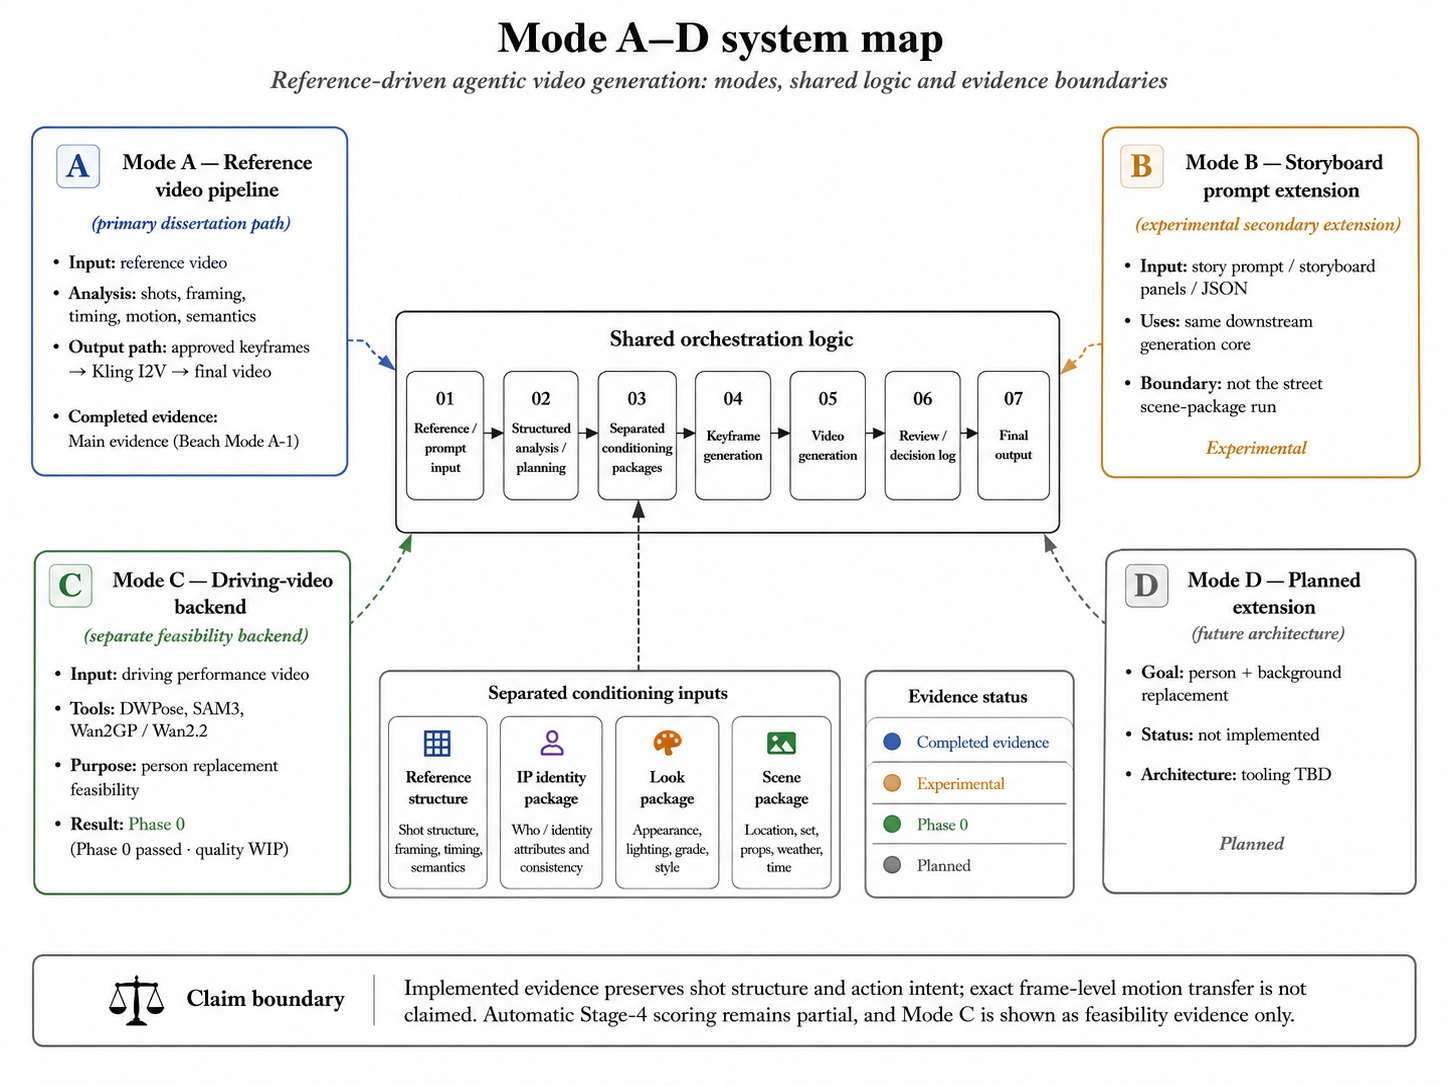
\includegraphics[width=\textwidth,height=0.85\textheight,keepaspectratio]{figs/system_overview_fig1.png}
\par\vspace{3pt}{\footnotesize \textbf{Figure 1} --- System overview: Mode A--D map. Modes A (reference-video pipeline, the primary dissertation path) and B (storyboard-prompt extension, experimental) share the same keyframe-first orchestration core and separated identity/look/scene conditioning packages; Mode C is a \emph{separate} driving-video backend (DWPose + SAM-style mask conditioning via Wan2.2-Animate/Wan2GP), probed as feasibility evidence only; Mode D (person + background replacement via hosted services) is a \emph{planned} extension and is \textbf{not implemented} --- only a dated hosted-service demo comparison is reported (\S{}4.18). The claim boundary applies across all modes: the implemented evidence preserves shot structure and action intent and does not claim exact frame-level motion transfer.}
\end{figure*}

\addcontentsline{toc}{subsection}{1.1 Motivation and background}

\section*{1.1 Motivation and background}

Short-form vertical video --- the 9:16 clips that dominate TikTok, Instagram Reels and YouTube Shorts --- is not usually authored from scratch. Creators study clips that already work and reuse their \emph{structure}: the number and order of shots, the cut rhythm, the framing of each shot, and the way motion lands on the beat. What changes between one creator's version and another is the \emph{content} --- the character, the outfit, the location --- not the underlying structure. A short is, to a first approximation, a small set of key poses and framings joined by beat-driven cuts.

Recent text-to-video and image-to-video models make it possible to generate such clips, but they do not support this reuse-of-structure workflow. A prompt goes in and a clip comes out as a single opaque unit. If one shot is wrong --- the character's identity drifts, the framing is off, a cut misses the beat --- there is no handle to inspect \emph{which} shot failed and no way to regenerate only that shot; the creator re-rolls the whole clip and hopes. Equally, a naive "AI watches a video and makes a video" approach either copies the reference too literally, raising derivative-work concerns, or discards its structure entirely and produces something unrelated. Neither extreme gives a controllable, auditable path from a reference clip to a new clip that keeps the reference's \emph{structure} while replacing its \emph{content} with a fixed, creator-owned IP character.

This gap is an \emph{orchestration} problem more than a generative-modelling problem. The individual capabilities exist --- shot detection, beat tracking, pose estimation, identity-conditioned image generation, image-to-video --- but they are not composed into a loop that decomposes a reference, regenerates content shot by shot, checks the result, and repairs what failed. Building that loop is the subject of this dissertation.

\addcontentsline{toc}{subsection}{1.2 Problem statement}

\section*{1.2 Problem statement}

The problem addressed is: given (i) a reference short-form video, (ii) a fixed IP character, and (iii) a target scene, produce a new 9:16 short that preserves the reference's shot structure and action intent while rendering the IP character in the target scene --- and do so through a controllable pipeline that can detect and repair individual failed shots, rather than a single end-to-end generation. The system must operate on closed generation APIs without training a model, because model training is out of scope for the timeline and hardware of an MSc project and is not the intended contribution.

\addcontentsline{toc}{subsection}{1.3 Research question}

\section*{1.3 Research question}

\emph{Can a reference short-form video be decomposed into a reusable structural template and regenerated with a fixed IP character under scene preservation and scene replacement, using a traceable human-gated evaluation--repair workflow over closed generation APIs; and what evidence does the decision log provide about selective repair compared with first-attempt outputs?}

\addcontentsline{toc}{subsection}{1.4 Aims and objectives}

\section*{1.4 Aims and objectives}

The aim is to design, build and honestly evaluate the pipeline above. The objectives are:

\begin{enumerate}[leftmargin=1.4em,itemsep=2pt,topsep=2pt]

\item Decompose a reference clip into a five-track, beat-aligned storyboard (shots, timing, framing, camera motion, character motion) using deterministic tools rather than model guessing (Stage 1--2).

\item Regenerate each shot with the IP character, keeping identity, look and scene as separate conditioning channels, keyframe first and then image-to-video (Stage 3).

\item Implement a human-gated evaluation--repair workflow, built on a shared decision-log schema, that diagnoses failures, repairs only the failed shot, and logs every decision to a state file with a \texttt{needs\_human} terminal state; specify the fully automatic, metric-driven version of this loop as the Stage-4 design target (Stage 4).

\item Evaluate identity, pose, framing and beat alignment where evidence permits; report the executed evidence --- human review, an ArcFace post-hoc identity diagnostic, a motion-energy audit and a decision-log reconstruction of first-attempt versus repaired outcomes --- against what remains pending (in-loop pose/framing/beat scoring and an independent equal-budget ablation), honestly.

\item Probe, as future-facing feasibility, a stronger structural backend (driving-video person replacement, Mode C).

\end{enumerate}

\addcontentsline{toc}{subsection}{1.5 Contributions}

\section*{1.5 Contributions}

This work contributes: (i) a reference-video decomposition into a five-track, beat-aligned storyboard representation computed by deterministic tools rather than LLM guessing; (ii) an IP-conditioned, keyframe-first per-shot regeneration pipeline that separates identity, look and scene; (iii) an agentic evaluation--repair loop with a per-shot decision log that repairs only the failed shot and records an explicit \texttt{needs\_human} terminal state; (iv) a graded structural-conditioning strategy that matches conditioning strength to the reliability of the reference pose per shot; and (v) an honest executed-versus-pending evaluation, including a negative result (skeleton-image guidance is too weak a control signal for the image API) and an identity-metric audit showing that a face-embedding metric mis-scores a synthetic character.

\addcontentsline{toc}{subsection}{1.6 Scope and boundaries}

\section*{1.6 Scope and boundaries}

The system is a proof of concept. It is evaluated on one reference video, four shots, one character and two scenes; multi-character interaction, fast action, occlusion, long-form and stylised content are not validated. It performs \emph{reference-structure-guided regeneration}, not pixel-level motion transfer: the reference supplies shot boundaries, framing, a broad camera-motion class, action intent and beat timing, but not per-frame limb trajectories. It is built on closed external services, so the \emph{architecture} is reproducible but the pixel-level output is bound to specific model versions and the execution date. Reference material is used for structure only and its pixels are not reproduced in the output. The target domain is vertical short-form video; the executed keyframe/video output is vertical \textbf{2:3} (768$\times$1152) rather than strict \textbf{9:16}, because \texttt{gpt-image-1} exposes only a fixed portrait size --- a platform-API limit stated here, not a target missed.

\addcontentsline{toc}{subsection}{1.7 Dissertation structure}

\section*{1.7 Dissertation structure}

Chapter 2 reviews the background and related work. Chapter 3 details the methodology: the four-stage agentic architecture, the reference analysis and template representation, IP-conditioned generation, the evaluation--repair loop, the state file and decision log, and the driving-video backend (Mode C). Chapter 4 reports the evaluation under the executed-versus-pending rule. Chapter 5 sets out the professional and ethical considerations. Chapter 6 concludes and sets out future work.

\par\vspace{22pt}
\Needspace*{12\baselineskip}
\addcontentsline{toc}{section}{Chapter 2 --- Background and Related Work}

\vspace*{2pt}\noindent{\LARGE\bfseries Chapter 2 --- Background and Related Work\par}\vspace{3pt}\hrule height 0.8pt\vspace{12pt}

\addcontentsline{toc}{subsection}{2.1 Structure in short-form video: a keyframing view}

\section*{2.1 Structure in short-form video: a keyframing view}

Short-form vertical video is characterised by rapid, beat-aligned cutting and a small number of strong key poses per clip. This structure is not incidental to the medium; it is a contemporary, algorithmically-distributed instance of principles that classical animation formalised decades ago, and reading it through that lens is what motivates the whole pipeline. Traditional animation distinguishes \emph{pose-to-pose} construction --- the animator first establishes the defining extreme poses, the \emph{keyframes}, and only then fills the in-betweens --- from \emph{straight-ahead} action drawn frame by frame (Thomas \& Johnston, 1981). Lasseter's foundational transfer of Disney's twelve principles to computer animation keeps that distinction central and adds \emph{timing} (how many frames a motion occupies, which sets its weight and legibility) and \emph{staging} (framing and composition that direct the viewer's attention to one idea at a time) as the levers that make a pose read on screen (Lasseter, 1987; Williams, 2001). Viewed this way, a short-form clip is close to a pure pose-to-pose sequence: a few readable key poses, each staged by its framing, joined by cuts whose timing is locked to a musical beat.

This framing does two things for the system. First, it makes the structure \emph{recoverable} by signal-level tools --- shot boundaries by content-based cut detection (Castellano, n.d.), beats by onset and tempo tracking (McFee et al., 2015), and character pose by 2D keypoint estimation (Lugaresi et al., 2019; Yang et al., 2023). Second, and more importantly, it dictates \emph{how to regenerate}. Rather than treating a clip as an indivisible sequence, the pipeline of Chapter 3 generates the defining keyframe of each shot first (a computational analogue of blocking key poses), aligns the cuts to a beat grid (timing), and carries an explicit per-shot framing track (staging) before any image-to-video in-betweening. The keyframe-first, beat-aligned design is therefore a direct, tool-driven realisation of pose-to-pose animation with explicit timing and staging, rather than an ad-hoc engineering convenience --- a point returned to when the creative-design intent of the system is set out in \S{}3.2.1.

\addcontentsline{toc}{subsection}{2.2 Identity-preserving image generation}

\section*{2.2 Identity-preserving image generation}

Preserving a fixed character across generations is the central difficulty, and the methods that address it form a clear historical progression in which each generation removes one cost and incurs another. The first generation was \emph{training-based}: DreamBooth (Ruiz et al., 2023) fine-tunes a whole diffusion model to bind a subject to a rare token, Textual Inversion (Gal et al., 2023) learns only a new embedding, and low-rank adaptation (LoRA) (Hu et al., 2022) learns a compact weight delta. These achieve strong, durable identity, but each requires per-subject optimisation, GPU training time and stored weights --- an awkward fit when the subject or the "look" changes frequently, as it does across an iterative creative project. The second generation was \emph{encoder-based} and training-free at inference: IP-Adapter (Ye et al., 2023) injects an image prompt through decoupled cross-attention, and InstantID (Wang et al., 2024), IP-Adapter FaceID and PhotoMaker (Li et al., 2024) specialise the idea for facial identity from as little as one reference. This removed per-subject training, but it introduced a second, and for this project decisive, assumption: every one of these methods needs \emph{access to the model's internals} --- its cross-attention layers, or a ControlNet/adapter hook --- that is, an open-weight checkpoint.

The present system deliberately operates one step removed from all of them, on a \emph{closed} image API (\texttt{gpt-image-1}) exposed only through an image-edit primitive with an \texttt{input\_fidelity} control (OpenAI, 2025) and no access to weights, embeddings or attention. None of the methods above can be applied directly. Identity must instead be pursued through the only levers the API exposes --- reference-image selection and ordering, prompt design, and fidelity control --- which is at once the constraint this dissertation works within (\S{}3.9) and a faithful model of how most applied teams actually consume generative models today: through a vendor endpoint rather than a checkpoint. The stronger open-weight methods are therefore positioned as future work rather than omitted. Face identity is measured here with a face-recognition embedding (Deng et al., 2019); Chapter 4 audits --- and partly rejects --- its reliability on a stylised synthetic character.

\addcontentsline{toc}{subsection}{2.3 Structural and pose conditioning}

\section*{2.3 Structural and pose conditioning}

Hard spatial control of diffusion generation is typically obtained with ControlNet (Zhang et al., 2023) or T2I-Adapter (Mou et al., 2024), which condition on a pose skeleton, depth or edge map. These require a model that exposes a control interface. A closed image-edit API does not: a skeleton supplied only as an image reference is a weak, soft signal, which the present work confirms as a negative result (\S{}3.5.5, \S{}4.12). This motivates the \emph{graded structural conditioning} of Chapter 3, where conditioning strength is matched to the per-shot reliability of the extracted pose rather than applied uniformly.

\addcontentsline{toc}{subsection}{2.4 Image-to-video and driving-video animation}

\section*{2.4 Image-to-video and driving-video animation}

Image-to-video models animate a still frame into a short clip; commercial systems (used here for assembly, \S{}3.5) and open models such as Stable Video Diffusion (Blattmann et al., 2023) and AnimateDiff (Guo et al., 2024) exemplify the class. A related line drives a target appearance with an explicit motion source: Animate Anyone (Hu et al., 2023) and MagicAnimate (Xu et al., 2024) animate a reference person from a driving pose sequence, and recent driving-video systems (Wan2.2-Animate, run here via the Wan2GP low-VRAM runner; Cheng et al., 2025; DeepBeepMeep, 2026) replace a performer with a target character while following the driving motion. These provide much stronger structural control than a single-keyframe image-to-video path, at the cost of local GPU hardware; the present work probes one such backend as a feasibility extension (Mode C, \S{}3.10, \S{}4.17) rather than as the main pipeline. The same model class is also exposed through hosted one-click consumer services (the official Wan platform's ``Transfer'' function; Viggle AI), where the conditioning channels are collapsed behind a single upload-and-generate interface; \S{}4.18 reports a dated comparison against two such services.

\addcontentsline{toc}{subsection}{2.5 Reference-analysis tooling}

\section*{2.5 Reference-analysis tooling}

The reference-analysis stage composes established tools: content-based shot detection (Castellano, n.d.), beat and tempo estimation (McFee et al., 2015), 2D pose estimation (Lugaresi et al., 2019; Yang et al., 2023), dense optical flow for a motion-energy audit (Farneb\"ack, 2003), and a face-recognition embedding for identity (Deng et al., 2019). The contribution is not these tools individually --- they are deterministic and well established --- but their \emph{synchronisation} into a single beat-aligned storyboard and their use as computed evidence rather than model guesses (\S{}3.3--3.4). One caveat from this literature is load-bearing for the evaluation: ArcFace (Deng et al., 2019) is calibrated on real human faces, so its embedding metric is not well-defined for a synthetic, stylised character. This project treats that as a hypothesis to test rather than an assumption, and confirms it empirically (\S{}4.8.1) --- a deliberately reflective use of the tooling rather than an uncritical one.

\addcontentsline{toc}{subsection}{2.6 Agentic LLM workflows and evaluation--repair loops}

\section*{2.6 Agentic LLM workflows and evaluation--repair loops}

The system is framed as an agentic workflow: tools compute and agents decide. This follows a line of work on tool-augmented reasoning and self-correction --- reasoning-and-acting agents (Yao et al., 2023), self-refinement (Madaan et al., 2023) and reflexion-style feedback (Shinn et al., 2023) --- in which a model inspects the result of an action and revises. The distinguishing feature here is that the loop is made \emph{auditable}: rather than an implicit chain of thought, every per-shot decision (scores, verdict, diagnosis, repair action, whether the retry improved) is written to a readable state file with an explicit \texttt{needs\_human} terminal state (\S{}3.7). This makes the "agentic" claim inspectable and turns the decision log into evaluation data. The present implementation is deliberately reported as a \emph{partially automated, human-gated} loop (\S{}4.15.1); a fully automatic scoring-driven loop is identified as future work.

Table 2.1 positions the system against six related clusters, each strong on one axis this project needs but unsuited on its own to a closed-API, per-shot-repairable pipeline.

\begin{table*}[t]
\centering
{\footnotesize\textbf{\textbf{Table 2.1 --- Related-work positioning}}}\par\vspace{3pt}
\footnotesize
\begin{tabularx}{\textwidth}{>{\RaggedRight\arraybackslash}X>{\RaggedRight\arraybackslash}X>{\RaggedRight\arraybackslash}X>{\RaggedRight\arraybackslash}X}
\toprule
Approach & Strength & Limitation for this project & This dissertation's response \\
\midrule
DreamBooth / LoRA (Ruiz et al., 2023; Hu et al., 2022) & Strong, trainable identity fidelity & Requires per-character training and GPU time outside project scope & Closed-API reference orchestration: identity held through reference images and role separation, not training \\
IP-Adapter / InstantID / PhotoMaker (Ye et al., 2023; Wang et al., 2024; Li et al., 2024) & Fast identity conditioning without full fine-tuning & Needs open-model adapter hooks unavailable on closed APIs & Identity anchors and fixed reference-slot ordering approximate the same role inside \texttt{images.edit} \\
ControlNet / T2I-Adapter (Zhang et al., 2023; Mou et al., 2024) & Hard, pixel-aligned pose control & Needs an open model with a control-map input; \texttt{gpt-image-1} exposes none & Graded soft guidance (\S{}3.5.5) now; the Mode C driving-video backend as the future hard-control route \\
I2V / Kling (Kuaishou Technology, 2024) & Accessible, production-grade image-to-video & Weak temporal/pose control from a single keyframe & Keyframe-first generation with a post-hoc motion-energy audit and prompt-only motion repair (\S{}4.13) \\
Driving-video person replacement (Cheng et al., 2025) & Genuine per-frame motion following & High GPU cost; a separate, non-keyframe-first backend & Reported as Mode C feasibility evidence, not integrated into the main pipeline \\
Agentic LLM workflows (Yao et al., 2023; Madaan et al., 2023; Shinn et al., 2023) & Self-correction from observed output & Correction is typically implicit or text-only, not logged against measurable per-shot criteria & Per-shot decision log with an explicit \texttt{needs\_human} terminal state (\S{}3.7) \\
\bottomrule
\end{tabularx}
\end{table*}

\addcontentsline{toc}{subsection}{2.7 Research gap}

\section*{2.7 Research gap}

Prior work clusters at two poles. One pole trains or fine-tunes generative models for identity or pose control, which requires GPU-scale training and targets model quality. The other pole performs uncontrolled end-to-end text-to-video generation with no per-shot handle. Comparatively little work composes \emph{deterministic reference decomposition} + \emph{IP-conditioned per-shot regeneration} + an \emph{auditable agentic repair loop} over \emph{closed} generation APIs, and evaluates it under an honest executed-versus-pending rule. That composition, and its honest evaluation, is the space this dissertation occupies.

\par\vspace{22pt}
\Needspace*{12\baselineskip}
\addcontentsline{toc}{section}{Chapter 3 --- Methodology and System Design}

\vspace*{2pt}\noindent{\LARGE\bfseries Chapter 3 --- Methodology and System Design\par}\vspace{3pt}\hrule height 0.8pt\vspace{12pt}

\addcontentsline{toc}{subsection}{3.1 Motivation and design rationale}

\section*{3.1 Motivation and design rationale}

\textbf{Contributions.} This work contributes: (i) a reference-video decomposition into a five-track, beat-aligned storyboard representation (shots, timing, framing, camera motion, character motion) computed by deterministic tools rather than LLM guessing; (ii) an IP-conditioned, keyframe-first per-shot regeneration pipeline that separates identity, look and scene; (iii) an agentic evaluation--repair loop with a per-shot decision log that repairs only the failed shot and records an explicit \texttt{needs\_human} terminal state; (iv) a graded structural-conditioning strategy that matches conditioning strength to the reliability of the reference pose per shot; and (v) an honest executed-vs-pending evaluation, including a negative result (skeleton-image guidance is too weak a control signal for \texttt{gpt-image-1}) and an identity-metric audit showing that a face-embedding metric under-scores a synthetic character a human reader accepts.

\addcontentsline{toc}{subsubsection}{3.1.1 From interactive assistance to reproducible orchestration}

\subsection*{3.1.1 From interactive assistance to reproducible orchestration}

A hosted conversational image assistant (for example, ChatGPT's image mode) implicitly performs reference-role interpretation, prompt expansion, running-intention retention across turns, and iterative self-correction from its own output --- a user uploads a few images, issues a terse instruction such as \emph{"keep this person, put her in a street scene, in this outfit"}, and a satisfactory result appears after a little invisible back-and-forth.

The OpenAI Images API exposes only the generation primitive underneath that experience: \texttt{images.edit} accepts source images and a prompt, but does not know which image should control identity, outfit, scene or framing. Left unguided, these references \emph{compete for control} and identity typically drifts while scene and outfit come through --- so the orchestration a hosted assistant hides has to be rebuilt explicitly outside the API.

That is precisely this dissertation's contribution, and it must be stated correctly: not to reproduce the hosted assistant's hidden helper --- which is \emph{opaque}, \emph{non-reproducible} and \emph{non-measurable} --- but to turn each hidden step into an \textbf{explicit, reproducible, auditable and measurable} component of an agentic orchestration layer. Reference roles, prompt blocks, slot order, review gates and repair decisions are written to the state file rather than hidden inside a conversational assistant: the API generates; the system decides, constrains, records (\S{}3.7) and repairs (\S{}3.6).

Table 3.1 maps each implicit step to the explicit component that realises it here.

\begin{table*}[t]
\centering
{\footnotesize\textbf{\textbf{Table 3.1 --- Implicit hosted-assistant steps vs. explicit pipeline components}}}\par\vspace{3pt}
\footnotesize
\begin{tabularx}{\textwidth}{>{\RaggedRight\arraybackslash}X>{\RaggedRight\arraybackslash}X}
\toprule
Implicit step (hosted assistant) & Explicit component (this system) \\
\midrule
Understand image content (face / outfit / background) & GPT-4o Vision semantic pass + source-frame structural anchor (Stage 1) \\
Hold the running "keep this person" intention & Identity anchor + locked \texttt{images.edit} slot order (slot \texttt{[0]} primary) \\
Expand a terse instruction into a strong visual prompt & Block-structured prompt (CHARACTER / LOOK / SCENE / FRAMING) \\
Decide which reference dominates & Fixed slot priority + input separation (identity / look / scene / source frame) \\
Suppress unwanted content & Forbidden-word guard (positive-only prompt; negatives stored, never sent) \\
"It doesn't look right --- try again" & Human review gate + decision log + evaluation$\rightarrow$repair loop \\
See the result and judge it & Evaluator: ArcFace identity, DWPose pose, framing, beat --- a \emph{score}, not a feeling \\
\bottomrule
\end{tabularx}
\end{table*}

The rest of this chapter details these components. The difference to keep in view is that where the hosted assistant \emph{feels} whether a result is right, this system \emph{measures} it (\S{}3.6) and records the decision (\S{}3.7), converting an opaque interaction into reproducible, evaluable evidence.

\addcontentsline{toc}{subsubsection}{3.1.2 Design principles}

\subsection*{3.1.2 Design principles}

The system is built as a \textbf{four-stage agentic pipeline} organised around a single, human-readable state file rather than as a linear generator or an ensemble of chat agents. The design follows one governing principle:

\begin{quotebox}\textbf{Tools compute; agents decide.}\end{quotebox}

Deterministic tools (shot-cut detection, beat tracking, pose estimation, face embedding, rendering) produce measurable signals. Language-model agents (Template Builder, Generation Planner, Evaluator, Repair Decision-Maker) consume those signals and take structured decisions that are written back to the state file. This separation is what allows the pipeline's behaviour to be audited: every decision is a logged transition over shared state, not an opaque conversation.

The task is framed narrowly and deliberately. It is \textbf{reference-video decomposition + IP-conditioned regeneration + an automatic evaluation--repair loop} --- not a general "AI watches a video and makes a video" generator. The reference video is analysed only for \emph{formal structure} (shot cuts, rhythm, framing, body orientation, timing); no reference pixels or reference audio appear in the output. This scoping is both a technical decision (structure is measurable and reusable; content is not) and a copyright decision (\S{}3.8).

The single feature that makes the system \emph{agentic} rather than a fixed pipeline is the feedback edge from Stage 4 back to Stage 3: \textbf{Evaluation $\rightarrow$ Generation}. A shot that fails evaluation is diagnosed and only that shot is regenerated, guided by the diagnosis. The rest of the sequence is untouched. Without this edge the system would be a one-shot generator; with it, the system reasons about its own output and repairs selectively.

\addcontentsline{toc}{subsection}{3.2 System architecture}

\section*{3.2 System architecture}

The pipeline has four stages and one shared artefact:

\begin{enumerate}[leftmargin=1.4em,itemsep=2pt,topsep=2pt]

\item \textbf{Reference Analysis} --- extract shot cuts, beats, camera-motion class, pose/motion, and framing from the reference video using deterministic tools.

\item \textbf{Template Builder} --- synchronise shot cuts, pose timestamps and audio beats into a single \textbf{beat-aligned storyboard JSON}.

\item \textbf{IP-Conditioned Generation} --- generate each shot from the fixed IP character plus a per-shot scene prompt, keyframe-first, then image-to-video, then assemble.

\item \textbf{Evaluation \& Repair} --- score each shot on identity, pose/motion, framing and beat alignment; on failure, diagnose and regenerate only the failing shot.

\end{enumerate}

All four stages read from and write to \textbf{\texttt{project\_state.json}}, the central state file (\S{}3.7). The system is delivered as a single Flask dashboard exposing two input modes that share this architecture: \textbf{Mode A} (reference video $\rightarrow$ shot analysis $\rightarrow$ IP-conditioned photoreal regeneration) and \textbf{Mode B} (natural-language prompt $\rightarrow$ animated storyboard sheet $\rightarrow$ panel review $\rightarrow$ JSON $\rightarrow$ video). This chapter documents Mode A, which exercises the full reference-decomposition pipeline; Mode B is described as a scoped variant in \S{}3.8.

\begin{figure*}[!tp]
\centering
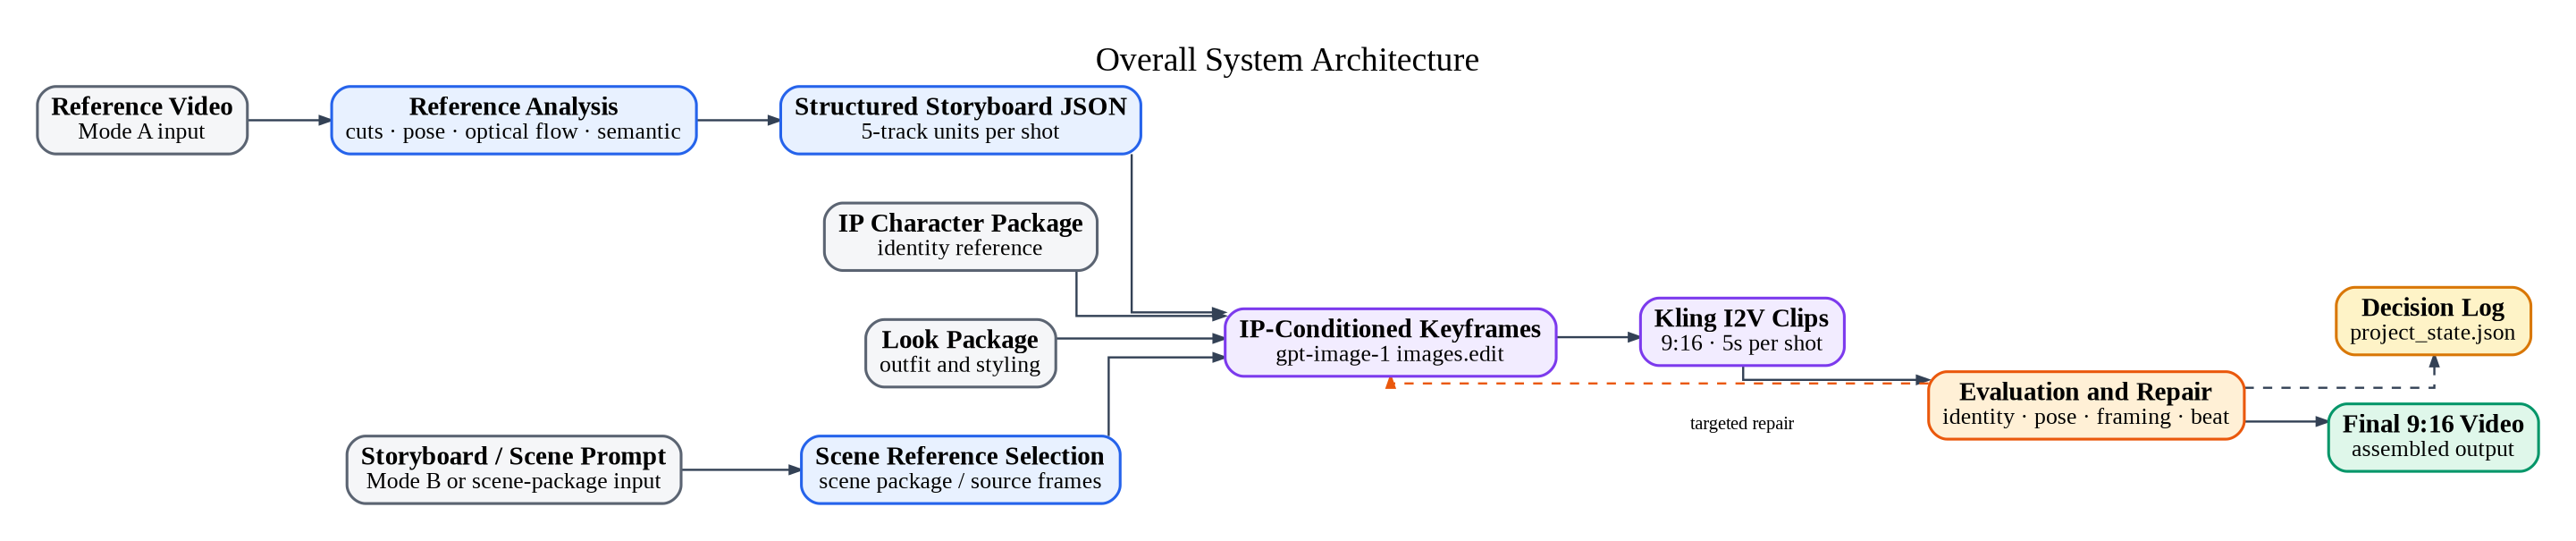
\includegraphics[width=\textwidth,height=0.85\textheight,keepaspectratio]{figs/overall_system_architecture_optimized.png}
\par\vspace{3pt}{\footnotesize \textbf{Figure 3.1} --- Overall system architecture: reference video $\rightarrow$ structured storyboard JSON $\rightarrow$ IP-conditioned keyframes $\rightarrow$ Kling I2V clips $\rightarrow$ evaluation \& repair, with the targeted-repair edge back into keyframe generation and the decision log written to \texttt{project\_state.json}.}
\end{figure*}

\addcontentsline{toc}{subsubsection}{3.2.1 Creative-design intent: character and look development}

\subsection*{3.2.1 Creative-design intent: character and look development}

Although this dissertation is framed as an engineering system, the artefact it produces is a piece of character-driven media, and several of its core mechanisms are creative-design decisions rather than purely technical ones. Making that design layer explicit is important both to the work's originality and to reading it as an animation project rather than a generic generation demo.

The first design decision is the IP character itself: a fixed, project-owned identity that the pipeline is built to reproduce consistently across shots and scenes. Designing such a character --- its facial structure, silhouette and a controlled set of \emph{looks} --- is a small but genuine act of character design and look development, the same discipline that in a production pipeline yields a character sheet and a set of approved looks before any shot is animated. In this system that practice is concretely embodied: the "Look 3" identity is captured not as a single image but as a small purpose-built reference set --- a front-facing facial anchor, a side/profile anchor, and outfit references --- each authored to control a specific axis of appearance.
The second design decision is the pipeline's \textbf{identity / look / scene separation} (\S{}3.5.1). Rather than a technical convenience, this mirrors how look development is organised in practice: \emph{who the character is} (identity), \emph{how they are dressed and styled for this piece} (look), and \emph{where the shot takes place} (scene) are treated as independent, separately-authored channels. This is what lets the same character be re-staged --- the completed beach demonstration and the Parisian-street run reuse one identity under two art directions --- and it is what makes a design change (a new look, a new location) a first-class, controllable operation rather than a re-roll.

The third is \textbf{staging as a per-shot design choice}. The framing track carried through the storyboard (over-shoulder medium, wide back-view, low-angle insert, side-profile) is a compositional decision in the animation sense of staging (Lasseter, 1987): each shot is framed to present one clear idea, and that framing is authored and repaired as deliberately as the identity is. Taken together, the character and its looks, the separation of design axes, and per-shot staging are the creative contribution that sits alongside the engineering one; the system is a tool for \emph{directing} a fixed character through a reference-derived structure, not only for synthesising frames.



\addcontentsline{toc}{subsubsection}{3.2.2 Formal pipeline specification}

\subsection*{3.2.2 Formal pipeline specification}

The narrative description above is restated here as pseudocode and a formal decision-log schema, so the pipeline's control flow and the evidence it produces are specified precisely rather than only described in prose.

\begin{algobox}{Algorithm 1: Reference decomposition (Stages 1--2)}
\textbf{Input:} reference video $V$\\
\textbf{Output:} five-track storyboard units $U=\{u_1,\dots,u_n\}$\\[2pt]
1: $C \leftarrow$ DetectCuts($V$) \quad\{PySceneDetect\}\\
2: $B \leftarrow$ ExtractBeats($V$) \quad\{librosa onset/tempo\}\\
3: \textbf{for} each shot $s \in C$ \textbf{do}\\
4: \quad $P_s \leftarrow$ SamplePose($s$, \{start,mid,end\})\\
5: \quad $M_s \leftarrow$ ClassifyCameraMotion($s$)\\
6: \quad $D_s \leftarrow$ DescribeSemantics($s$) \quad\{enrichment only\}\\
7: \quad $t_s \leftarrow$ SnapToBeat($s$.cut\_time, $B$, $\tau_{\text{snap}}$)\\
8: \quad\quad \{keep original cut if no beat within $\tau_{\text{snap}}$\}\\
9: \quad $u_s \leftarrow$ BuildUnit($s,P_s,M_s,D_s,t_s$)\\
10: \textbf{end for}\\
11: $U \leftarrow$ ValidateCompleteness($\{u_s\}$)\\
12: \textbf{return} $U$
\end{algobox}

\begin{algobox}{Algorithm 2: Per-shot regeneration (Stage 3)}
\textbf{Input:} unit $u_i$, identity package $I$, look $L$, scene $S$\\
\textbf{Output:} approved keyframe $k_i$, clip $c_i$\\[2pt]
1: slots $\leftarrow$ OrderReferenceSlots($I,L,S,u_i$.source\_frame)\\
2: \quad\{fixed priority; slot[0] = primary identity\}\\
3: prompt $\leftarrow$ BuildPromptBlocks($u_i,I,L,S$)\\
4: \quad\{CHARACTER / LOOK / SCENE / FRAMING / ACTION / NEGATIVE\}\\
5: attempt $\leftarrow 0$\\
6: \textbf{repeat}\\
7: \quad attempt $\leftarrow$ attempt $+1$\\
8: \quad $k \leftarrow$ ImagesEdit(slots, prompt) \quad\{\texttt{gpt-image-1}\}\\
9: \quad verdict $\leftarrow$ HumanReview($k$)\\
10: \quad \textbf{if} verdict $=$ reject \textbf{then}\\
11: \quad\quad issue $\leftarrow$ Diagnose($k,u_i$)\\
12: \quad\quad prompt $\leftarrow$ Revise(prompt, issue) \quad\{targeted, not blind re-roll\}\\
13: \quad \textbf{end if}\\
14: \textbf{until} verdict $=$ approve\\
15: LogAttempt($u_i$.shot\_id, attempt, issue, prompt, verdict)\\
16: $c \leftarrow$ KlingI2V($k, u_i$.character\_motion) \quad\{prompt-level I2V\}\\
17: \textbf{return} $k, c$
\end{algobox}

\begin{algobox}{Algorithm 3: Evaluation--repair loop (designed Stage 4)}
\textbf{Input:} generated shot $g_i$, metrics $\mathcal{M}=\{\text{identity},\text{pose},\text{framing},\text{beat}\}$, thresholds $\tau$\\
\textbf{Output:} accepted shot or \texttt{needs\_human}\\[2pt]
1: scores $\leftarrow$ ComputeMetrics($g_i,\mathcal{M}$)\\
2: \textbf{if} all scores $\geq \tau$ \textbf{then}\\
3: \quad mark $g_i$ \texttt{accepted}\\
4: \textbf{else}\\
5: \quad diagnosis $\leftarrow$ DiagnoseFailure(scores, $\tau$)\\
6: \quad \textbf{if} RepairBudget($g_i$) $> 0$ \textbf{then}\\
7: \quad\quad action $\leftarrow$ PlanRepair(diagnosis)\\
8: \quad\quad $g_i' \leftarrow$ Regenerate($g_i$, action)\\
9: \quad\quad LogDecision($g_i$.shot\_id, diagnosis, action, $g_i, g_i'$)\\
10: \quad\quad \textbf{return} Evaluate($g_i'$) \quad\{recurse, budget $-1$\}\\
11: \quad \textbf{else}\\
12: \quad\quad mark $g_i$ \texttt{needs\_human}\\
13: \quad \textbf{end if}\\
14: \textbf{end if}
\end{algobox}

\textbf{Executed-versus-designed boundary (restated formally).} Algorithms 1 and 2 above are executed exactly as specified. In Algorithm 3, lines 1--2 (automatic metric scoring against $\tau$) are the \emph{designed} form of the loop; on the executed runs, HumanReview($g_i$) --- the same gate used inside Algorithm 2 --- stands in for lines 1--2, and diagnosis/repair/logging (lines 5, 7--9) run exactly as specified under that substitution. This is the precise sense in which the system is a \emph{partially automated, human-gated} agentic loop (\S{}4.15.1): the control-flow skeleton of Algorithm 3 is executed end to end; only the scoring predicate that decides line 2 is currently supplied by a human rather than $\mathcal{M}$.

\addcontentsline{toc}{subsubsection}{3.2.3 Formal decision-log schema}

\subsection*{3.2.3 Formal decision-log schema}

Every attempt written to \texttt{project\_state.json} (\S{}3.7) conforms to one schema, given here formally rather than only by example.

\textbf{Attempt record.} \texttt{\{shot\_id, attempt\_id, model, slot\_config, prompt, observed\_issue, repair\_action, review\_status, retained\_output\}}, where \texttt{review\_status} $\in \{$\texttt{approved}, \texttt{rejected}, \texttt{pending}$\}$.

\textbf{Failure taxonomy} (observed values of \texttt{observed\_issue} across the executed runs): forbidden-word-guard block (positive/negative prompt conflict); source-frame/pose mismatch (described pose does not match the actual reference frame); look/garment mismatch (generated outfit diverges from the specified look package); under-motion (optical-flow energy below the shot's reference target, \S{}4.13); \texttt{unavailable\_no\_pose\_seed} (no usable pose detected for a shot, \S{}4.11.1); operational fault (e.g.\ remote GPU driver failure during a Mode~C run, \S{}4.17).

\textbf{Repair-action taxonomy}: \emph{identity repair} (re-prioritise identity anchors, reduce competing references); \emph{motion repair} (revise motion wording, keyframe retained); \emph{slot/prompt repair} (re-order reference slots or rewrite prompt blocks per Algorithm 2, line 12); \emph{control-signal boundary} (a signal is archived rather than forced into the final output, e.g.\ \S{}3.5.5); \emph{automation boundary} (an unexecuted automatic step is labelled designed future work rather than reported as completed).

\textbf{Terminal states}: \texttt{approved} (retained in the final assembly); \texttt{needs\_human} (repair budget exhausted without an accepted result); \texttt{archived} (a tested branch intentionally excluded from the final output, e.g.\ the pose-guidance branch of \S{}3.5.5).

\textbf{Invariants.} (i) A shot cannot reach \texttt{approved} without a recorded \texttt{review\_status} from either human review or, in the designed automatic form, $\mathcal{M} \geq \tau$. (ii) A shot that fails review must transition to either a further logged attempt or \texttt{needs\_human}; it cannot leave the log without a terminal state. (iii) Every repair action logs its \texttt{observed\_issue}, \texttt{repair\_action} and the resulting \texttt{review\_status} of the retry, so no repair is unattributed. (iv) A metric or ablation not computed in-loop is labelled \texttt{pending} in the record, never given a fabricated value --- the executed-versus-pending reporting rule applied throughout Chapter 4 is, at the data-schema level, enforcement of this invariant.

\addcontentsline{toc}{subsection}{3.3 Stage 1 --- Reference Analysis}

\section*{3.3 Stage 1 --- Reference Analysis}

Stage 1 converts the reference clip into structured, per-shot signal. It runs a bank of deterministic tools and merges their outputs conservatively; it does \textbf{not} ask a language model to guess shot boundaries or motion.

\begin{table*}[t]
\centering
\footnotesize
\begin{tabularx}{\textwidth}{>{\RaggedRight\arraybackslash}X>{\RaggedRight\arraybackslash}X>{\RaggedRight\arraybackslash}X}
\toprule
Signal & Tool / method & Output \\
\midrule
Shot cuts & PySceneDetect & Cut list with timestamps \\
Beats / tempo & librosa & Beat grid, BPM \\
Camera motion & Optical-flow classifier & Discrete camera-motion class (e.g. push-in, static) \\
Pose / character motion & MediaPipe keypoints & Per-shot body orientation and motion type \\
Semantic description & GPT-4o Vision & Framing / content labels per shot \\
\bottomrule
\end{tabularx}
\end{table*}

On the reference run, a 7.92 s, 30 fps, 123 bpm four-shot beach-sunset clip was decomposed into \textbf{four shots} with per-shot duration, framing class and camera-motion class. Signals from independent tools are combined by a \textbf{conservative multi-signal merge}: where tools disagree, the pipeline prefers the more reliable structural signal (the detected cut) over weaker inferred signals, rather than averaging them. This keeps the extracted template honest about what was actually measured.

Two properties of Stage 1 are load-bearing for the honesty of the whole system. First, camera motion and character motion are \textbf{estimated heuristically} --- the optical-flow class and the MediaPipe-derived motion type are categorical, not exact trajectories. Second, the semantic layer (GPT-4o Vision; OpenAI, 2024) is used only for description and enrichment; it never overrides a deterministic measurement. These are stated as limitations in the evaluation chapter, not hidden.

\begin{figure*}[!tp]
\centering
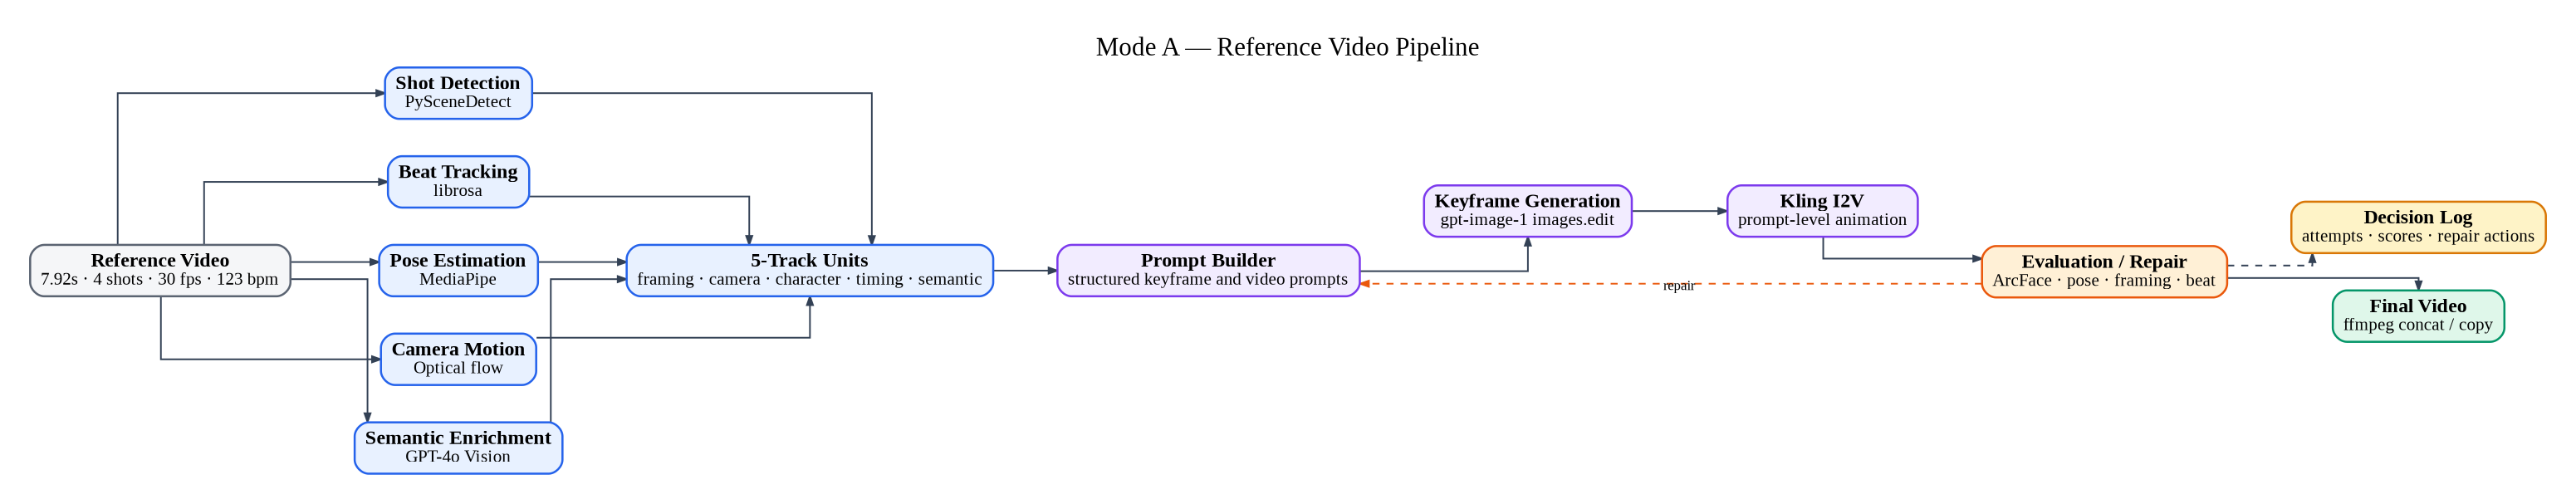
\includegraphics[width=\textwidth,height=0.85\textheight,keepaspectratio]{figs/mode_a_reference_video_pipeline_optimized.png}
\par\vspace{3pt}{\footnotesize \textbf{Figure 3.2} --- Mode A reference-video pipeline: the deterministic analysis bank (PySceneDetect, librosa, MediaPipe, optical flow, GPT-4o Vision) feeds the five-track units and prompt builder, then keyframe generation, Kling I2V, evaluation/repair, and ffmpeg assembly.}
\end{figure*}

\addcontentsline{toc}{subsubsection}{3.3.1 Start--middle--end pose sampling for temporal shot structure}

\subsection*{3.3.1 Start--middle--end pose sampling for temporal shot structure}

In the initial implementation, each detected shot was represented by a single \textbf{middle frame}. This is enough to fix a representative composition, but it does not capture how the subject's pose and orientation change \emph{within} a shot. Stage 1 was therefore extended to sample \textbf{three frames per shot} --- start, middle and end --- and to run MediaPipe Pose on each, recording per-frame pose confidence and keypoint count alongside the keypoints themselves. On the reference clip (237 frames, 30 fps) this yields twelve pose samples across the four shots.

The purpose of this sampling is not to drive generation directly but to \textbf{measure how reliable pose is for each shot before deciding how much to trust it} --- a "tools compute, agents decide" step. Pose reliability varies sharply by shot type (reported quantitatively in \S{}4.11): full-body walking shots yield stable skeletons, whereas close-up and feet-only shots yield sparse or empty detections. This measurement is what makes the graded structural-guidance policy of \S{}3.5.5 possible: rather than assuming every shot can be pose-guided, the system first checks pose quality per shot and selects a conditioning strength accordingly. (This analysis writes to a separate report and does not itself modify \texttt{project\_state.json} or call any paid API.)

\addcontentsline{toc}{subsection}{3.4 Stage 2 --- Template Builder (beat-aligned storyboard)}

\section*{3.4 Stage 2 --- Template Builder (beat-aligned storyboard)}

Stage 2 is the contribution that is easy to under-sell as "format conversion" but is not. It takes three time-stamped signal streams --- \textbf{shot cuts}, \textbf{pose timestamps} and \textbf{audio beats} --- and synchronises them into a single beat-aligned storyboard JSON. Each shot becomes a \textbf{generation unit} carrying five parallel tracks:

\begin{itemize}[leftmargin=1.2em,itemsep=2pt,topsep=2pt]

\item \texttt{framing} --- shot size / composition

\item \texttt{camera\_motion} --- camera-motion class from Stage 1

\item \texttt{character\_motion} --- body orientation / motion type

\item \texttt{timing} --- shot duration and its position on the beat grid

\item \texttt{semantic} --- content / scene description

\end{itemize}

On the reference run all four units reached \texttt{track\_completeness = full}.

The alignment step snaps shot cuts to the nearest audio beat, but under an explicit \textbf{maximum snap distance}. If a cut lies within the threshold of a beat, it is snapped and the timing is beat-locked; if the nearest beat is \emph{too far}, the \textbf{original cut is kept} rather than forcing a musically wrong alignment. This guard is deliberate: forcing every cut onto a beat would corrupt the timing of shots that were never beat-driven in the reference. The storyboard therefore records, per shot, whether its timing is beat-locked or cut-preserved --- this distinction later feeds the beat-alignment metric in Stage 4.

\begin{figure*}[!tp]
\centering
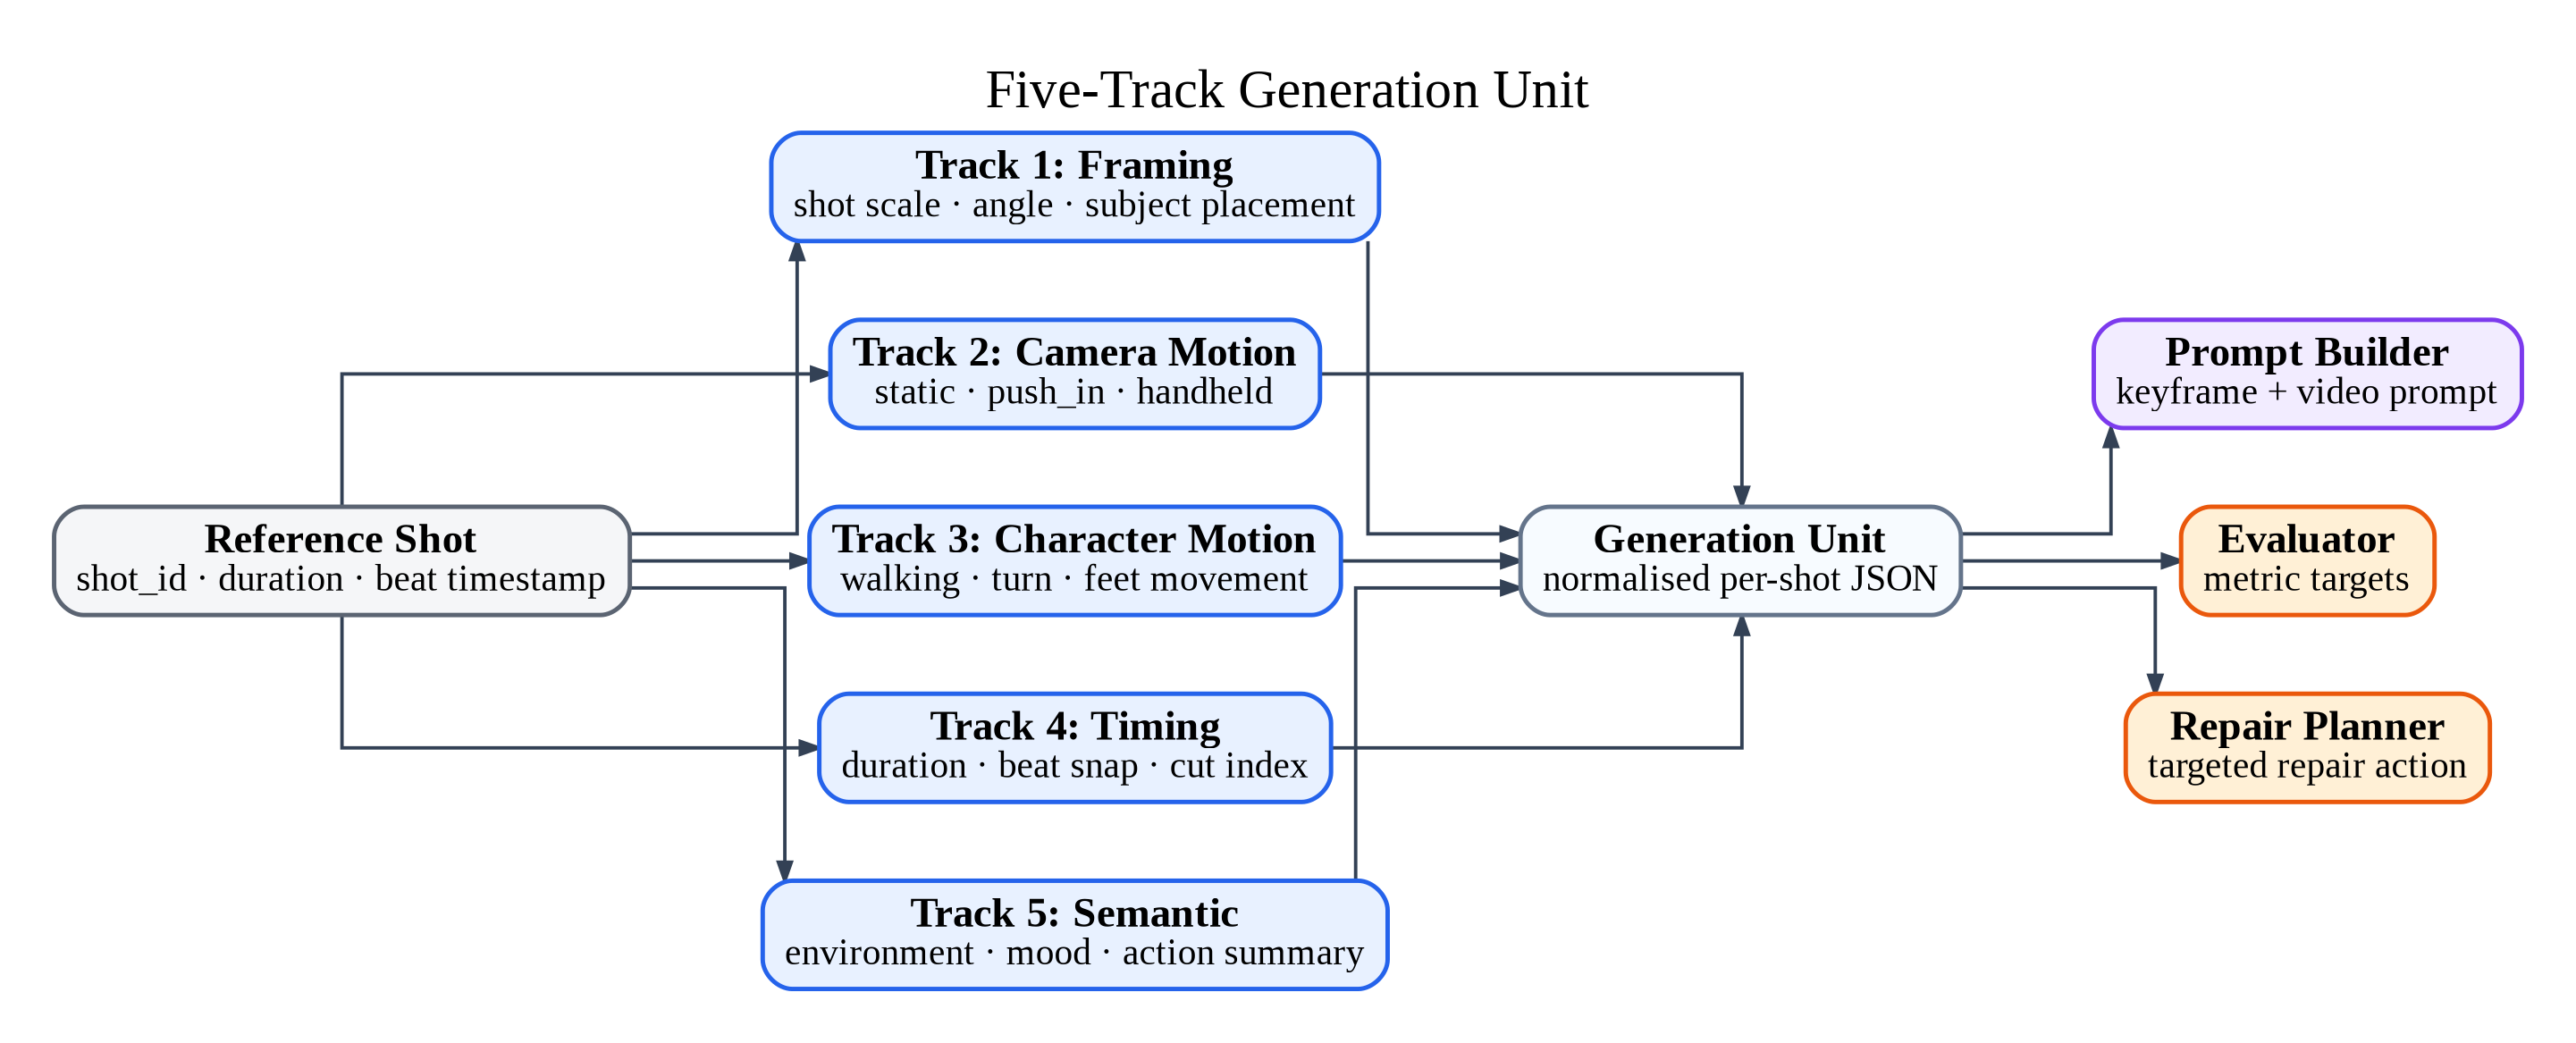
\includegraphics[width=\textwidth,height=0.85\textheight,keepaspectratio]{figs/five_track_generation_unit_optimized.png}
\par\vspace{3pt}{\footnotesize \textbf{Figure 3.3} --- Five-track generation unit: each reference shot (\texttt{shot\_id}, duration, beat timestamp) expands into framing, camera-motion, character-motion, timing and semantic tracks, normalised into a per-shot JSON that feeds the prompt builder, evaluator and repair planner.}
\end{figure*}

\addcontentsline{toc}{subsection}{3.5 Stage 3 --- IP-Conditioned Generation}

\section*{3.5 Stage 3 --- IP-Conditioned Generation}

Stage 3 regenerates each shot with the fixed IP character in the new scene. It is \textbf{keyframe-first}: the pipeline first produces one approved keyframe per shot, then animates that keyframe to a clip, then assembles the clips. Generation is always \textbf{per-shot, never one-shot-whole-video}, so that a single failed shot can be repaired without re-rolling the sequence.

\addcontentsline{toc}{subsubsection}{3.5.1 Identity / look / scene / source-frame separation}

\subsection*{3.5.1 Identity / look / scene / source-frame separation}

A shot's conditioning is factored into four independent sources so that each can be controlled and, on failure, adjusted in isolation: the \textbf{IP identity} (who the character is), the \textbf{look} (the specific outfit/styling for this run), the \textbf{scene} (environment/lighting), and the \textbf{source frame} (structural anchor from the reference). Keeping these separate is what lets the repair layer target one axis --- e.g. fix the outfit without disturbing identity or framing.

\begin{figure*}[!tp]
\centering
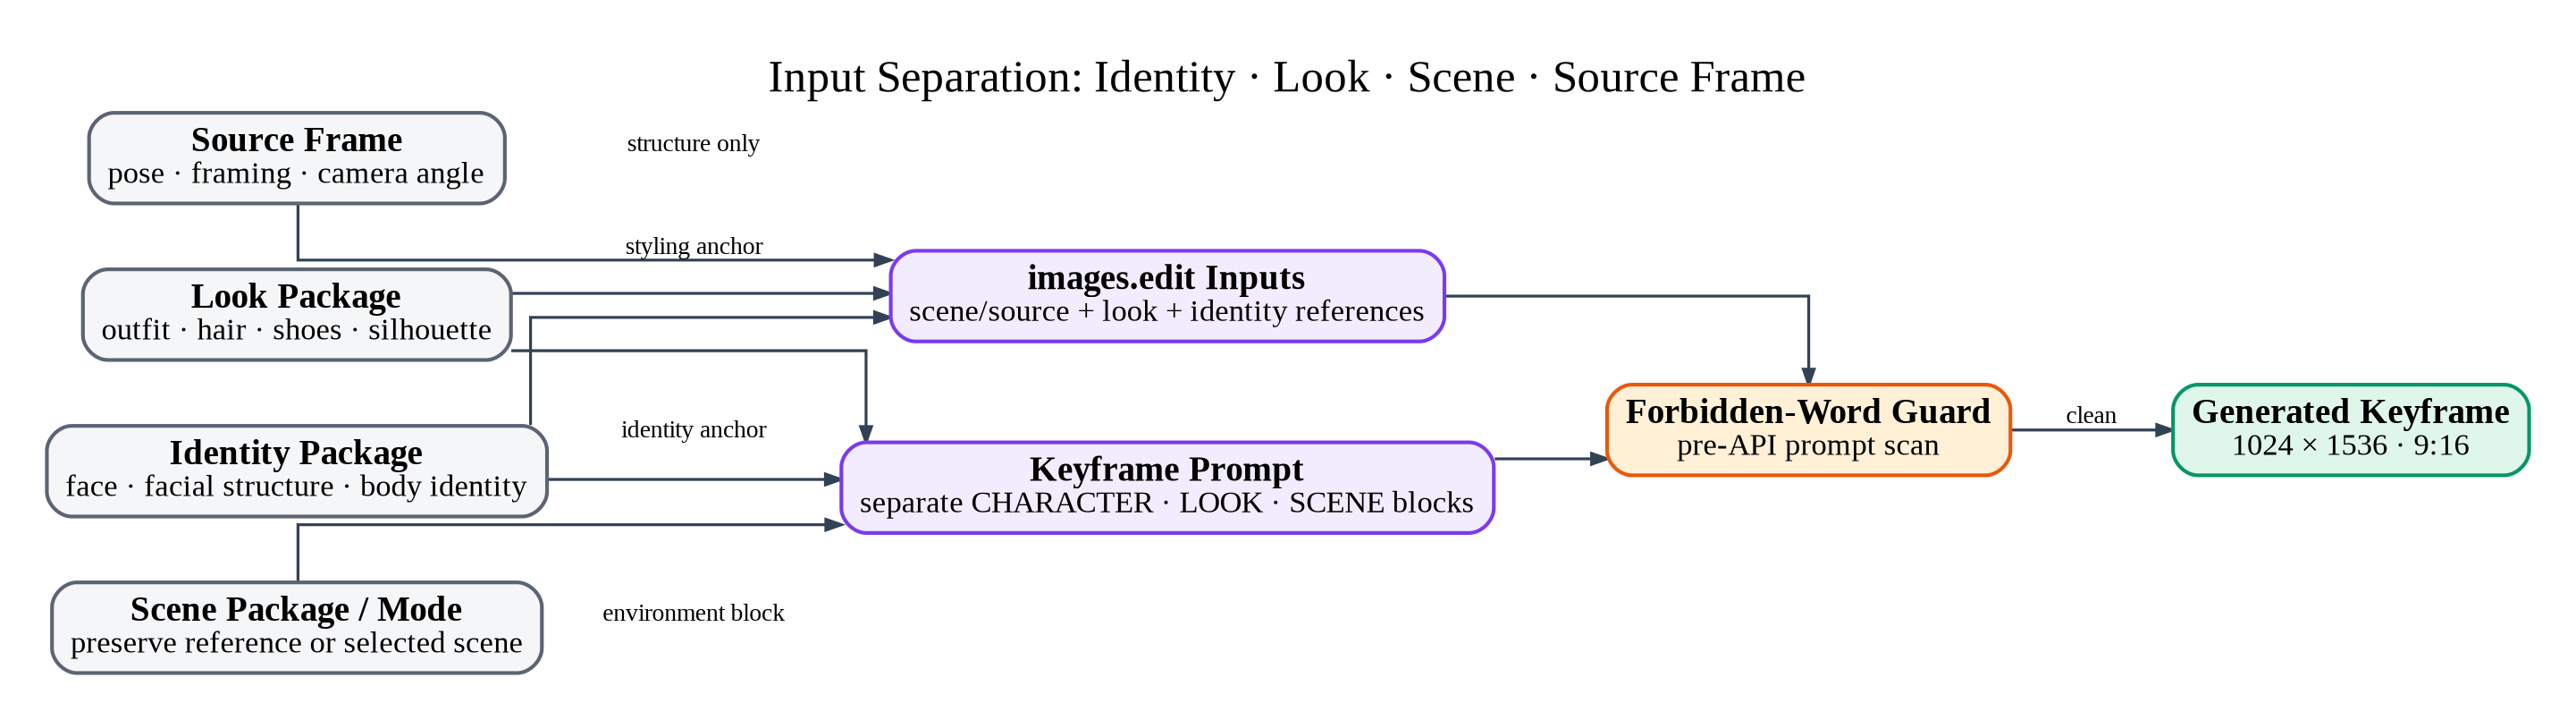
\includegraphics[width=\textwidth,height=0.85\textheight,keepaspectratio]{figs/identity_look_scene_source_frame_separation_optimized.png}
\par\vspace{3pt}{\footnotesize \textbf{Figure 3.4} --- Input separation: source frame (structure only), look package, identity package and scene package/mode are kept as independent conditioning sources feeding the \texttt{images.edit} inputs and the block-structured keyframe prompt, gated by the forbidden-word guard.}
\end{figure*}

\addcontentsline{toc}{subsubsection}{3.5.2 Keyframe generation}

\subsection*{3.5.2 Keyframe generation}

Keyframes are generated with \texttt{gpt-image-1} via the \texttt{images.edit} endpoint at 1024$\times$1536, medium quality by default. (The street identity-repair run raises this for identity-critical face-visible shots, using \texttt{quality="high"} and \texttt{input\_fidelity="high"} to strengthen facial preservation; see \S{}4.12.) Each keyframe is conditioned on \textbf{four input images in a locked slot order}:

\begin{table*}[t]
\centering
\footnotesize
\begin{tabularx}{\textwidth}{ll>{\RaggedRight\arraybackslash}X}
\toprule
Slot & Content & Role \\
\midrule
\texttt{[0]} & Source frame & \textbf{Primary} structural anchor (framing, body scale, camera distance) \\
\texttt{[1]} & Look front/body & Outfit reference \\
\texttt{[2]} & Look sheet & Look overview \\
\texttt{[3]} & Look close-up & Face reference \\
\bottomrule
\end{tabularx}
\end{table*}

The slot order is fixed because slot \texttt{[0]} carries the strongest structural weight; anchoring on the source frame is what preserves the reference's composition while the character and scene are replaced. One principled exception was applied on the reference run: for a \textbf{feet-only shot} (shot\_003) where the face is out of frame, the face close-up was left in the weakest slot \texttt{[3]} to avoid "face-bleed" into a shot that should contain no face.

Scene continuity is controlled by a \texttt{scene\_mode} flag. The reference run used \texttt{scene\_mode = preserve\_reference\_scene}, so the beach-sunset environment, wet sand, warm amber light and ocean horizon were rendered consistently across all four keyframes with no stale scene prompts injected.

A \textbf{forbidden-word guard} runs on every keyframe prompt. Only a positive prompt is sent to the image API; the negative prompt (identity-drift and unwanted-content terms) is stored separately in state and \textbf{never} passed to the API. This both satisfies the image model's input contract and keeps a clean, auditable record of what was and was not requested. On the reference run this guard is itself part of the decision log: shot\_002's first attempt was blocked pre-API because bridal terms sat in the negative instructions, and was resolved by separating positive from negative language.

\begin{figure*}[!tp]
\centering
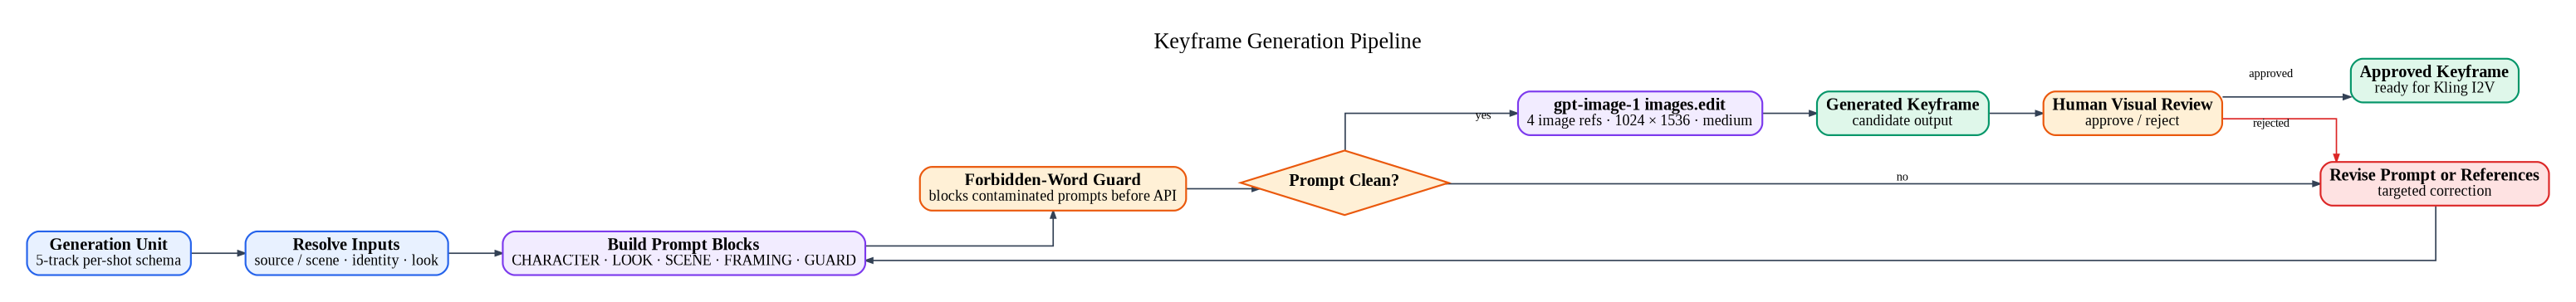
\includegraphics[width=\textwidth,height=0.85\textheight,keepaspectratio]{figs/keyframe_generation_pipeline_optimized.png}
\par\vspace{3pt}{\footnotesize \textbf{Figure 3.5} --- Keyframe generation pipeline, including the forbidden-word guard (blocks contaminated prompts before the API) and the human visual review approve/reject gate that routes rejected candidates to a targeted prompt/reference revision --- the keyframe-approval loop that operated on the reference run (\S{}3.7).}
\end{figure*}

\addcontentsline{toc}{subsubsection}{3.5.3 Image-to-video and assembly}

\subsection*{3.5.3 Image-to-video and assembly}

Each approved keyframe is animated with \textbf{Kling v1.6} (standard mode, 9:16, 5 s clips; Kuaishou Technology, 2024) driven by a natural-language \textbf{video prompt} describing the intended motion (walk direction, camera movement, body pose). Clips are concatenated by \texttt{ffmpeg} (FFmpeg developers, n.d.) with stream copy (no re-encode) into the final vertical short (768$\times$1152 / 20.4 s on the reference run).

An honesty boundary is fixed here and carried into every claim about the system:

\begin{quotebox}\textbf{The system preserves reference shot structure and action intent, but does not perform exact frame-level motion transfer.}\end{quotebox}

Motion is \textbf{prompt-level image-to-video}, not skeleton- or optical-flow-conditioned pose transfer. No per-frame keypoint sequence, ControlNet pose map or flow field is transmitted to the video model. Step cadence, exact stride length and inter-frame body position are therefore not controlled; only action \emph{intent} is. This is the designed behaviour of the current Mode A pipeline, and it reflects a deliberate scoping decision discussed next.

\begin{figure*}[!tp]
\centering
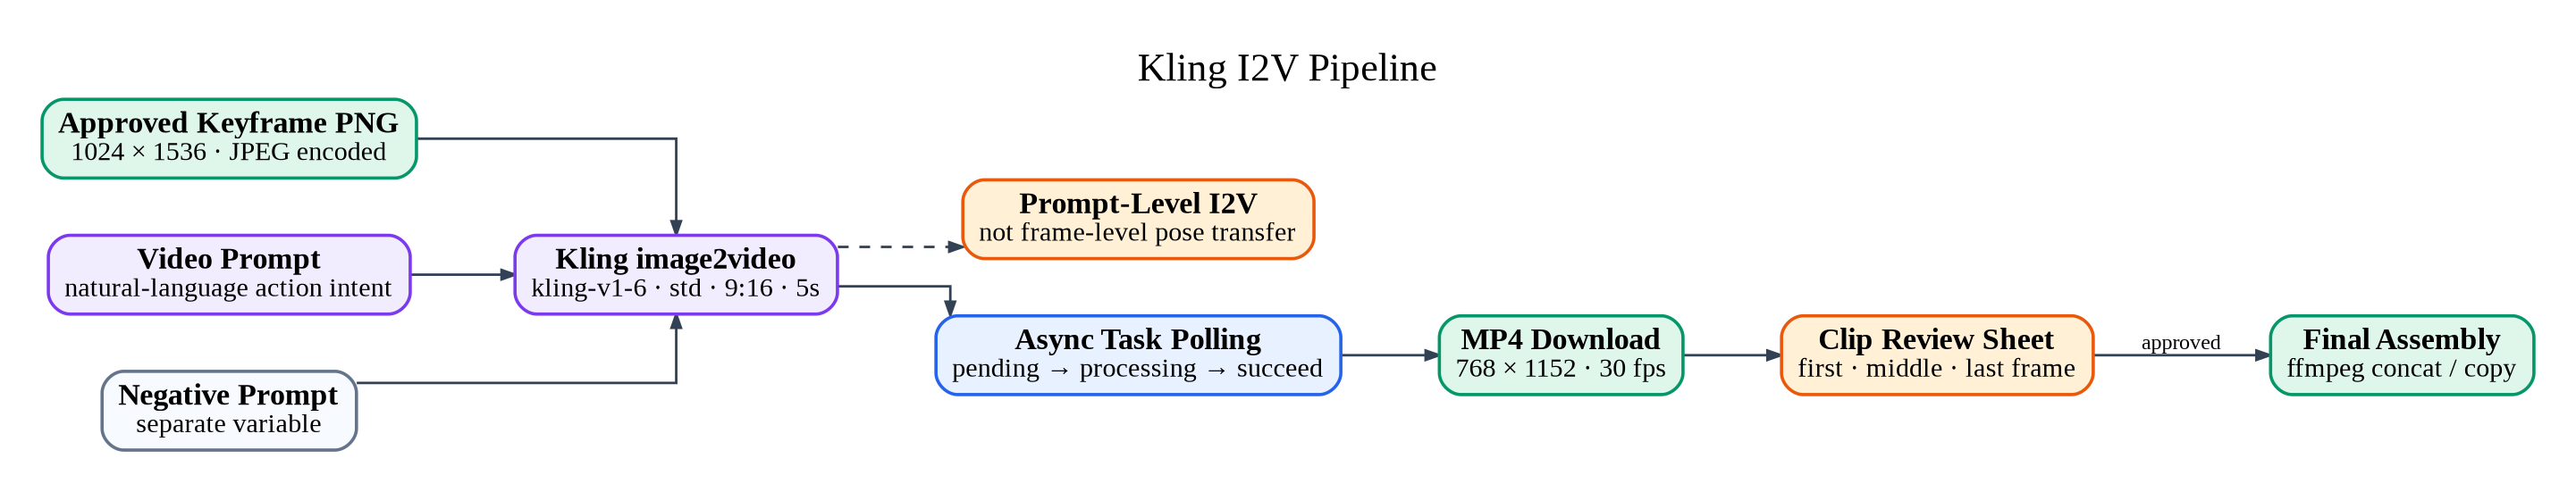
\includegraphics[width=\textwidth,height=0.85\textheight,keepaspectratio]{figs/kling_i2v_pipeline_optimized.png}
\par\vspace{3pt}{\footnotesize \textbf{Figure 3.6} --- Kling I2V pipeline: the approved keyframe (1024$\times$1536) plus a natural-language video prompt and a separately stored negative prompt drive \texttt{kling-v1-6} (prompt-level I2V, \emph{not} frame-level pose transfer); async polling $\rightarrow$ MP4 (768$\times$1152, 30 fps) $\rightarrow$ clip review $\rightarrow$ ffmpeg assembly.}
\end{figure*}

\addcontentsline{toc}{subsubsection}{3.5.4 Scoping note: pose control vs. identity}

\subsection*{3.5.4 Scoping note: pose control vs. identity}

The project's identified make-or-break risk is the tension between \textbf{strong pose conditioning} (which preserves motion) and \textbf{character identity} (which strong pose conditioning can distort). The planned Phase 0 feasibility test --- IP reference + pose skeleton + simple scene, checking that identity holds across poses against a pre-defined quantitative threshold --- was \textbf{not run} before the reference build. In line with the pre-committed fallback, the pipeline was therefore scoped to \textbf{keyframe-first generation with prompt-level I2V} rather than full skeleton-driven motion transfer. This is treated as a scoping decision, not a failure: a short-form vertical clip is, structurally, a sequence of key poses plus beat-driven cuts, and the keyframe-first route delivers that while sidestepping the identity-distortion risk of aggressive pose conditioning. Full pose-transfer is documented as future work (\S{}3.9), and the identity-vs-pose evaluation it would require is specified in \S{}3.6.

\addcontentsline{toc}{subsubsection}{3.5.5 Graded structural guidance (pose as soft conditioning)}

\subsection*{3.5.5 Graded structural guidance (pose as soft conditioning)}

Because \texttt{gpt-image-1} exposes no hard structural-control interface --- there is no ControlNet-style pose-map input to \texttt{images.edit} --- the system does \textbf{not} attempt exact pose transfer. Instead, pose is used as \textbf{soft, graded-strength structural guidance}, realised through two channels of differing strength:

\begin{enumerate}[leftmargin=1.4em,itemsep=2pt,topsep=2pt]

\item \textbf{Pose-derived textual cues} --- orientation, body direction, gait phase and walking posture, distilled from the keypoints into the natural-language prompt. \emph{(Implemented: such cues already appear in the per-shot prompts, e.g. "natural walking stride", "side profile, raised foot mid-stride".)}

\item \textbf{Identity-neutral skeleton reference image} --- the keypoints rendered as a clean stick-figure skeleton on a neutral background and supplied as an additional \texttt{images.edit} slot for pose-driven shots, so that structure is conveyed without leaking the reference's identity or scene. \emph{(Implemented and tested in the street start/end system (\texttt{generate\_street\_start\_end.py}) on the pose-reliable shots (shot\_002, shot\_004); the beach run used channel 1 only. On inspection \texttt{gpt-image-1} treated the skeleton as weak guidance and did not reliably follow it, so the branch was }\emph{archived and excluded from the final output}\emph{ (\S{}4.12).)}

\end{enumerate}

Beyond these two channels, per-sample pose detection paired with pose-seeded foreground \textbf{person-mask} candidates was explored as a possible route to stronger structure guidance and is documented as a local pose/mask audit in \S{}4.11.1; both are treated as \textbf{candidate control signals and diagnostic evidence} only, not hard control. These signals combine with the \textbf{identity anchors} and \textbf{scene package} so that structure, identity and environment are contributed by separate, controllable sources, with channel strength set per shot from the pose-reliability measurement of \S{}3.3.1 (reliable full-body shots take strong guidance, close-ups fall back to orientation cues, detail inserts use framing/text alone; per-shot grading in \S{}4.11).

The honest reading is therefore \textbf{structure-guided regeneration, not motion cloning}: shot structure and action intent are preserved through guidance compatible with the current model's capabilities, without a guarantee of frame-level agreement with the reference motion. A ControlNet-class or driving-video backend remains the route to stronger control (\S{}4.15, \S{}6.5).

\addcontentsline{toc}{subsection}{3.6 Stage 4 --- Evaluation and Repair}

\section*{3.6 Stage 4 --- Evaluation and Repair}

Stage 4 is what closes the loop. It scores each generated shot, decides a verdict, and --- on failure --- diagnoses the cause and triggers a targeted regeneration of only that shot. The metrics are defined as follows:

\begin{table*}[t]
\centering
\footnotesize
\begin{tabularx}{\textwidth}{>{\RaggedRight\arraybackslash}X>{\RaggedRight\arraybackslash}X>{\RaggedRight\arraybackslash}X}
\toprule
Metric & Method & Interpretation \\
\midrule
IP identity consistency & ArcFace cosine similarity (face-embedding metric), generated vs. IP reference & Higher similarity = identity held \\
Pose / motion similarity & Keypoint distance (DWPose on generated keyframe) vs. source-frame pose & Lower = closer to reference motion \\
Framing accuracy & Composition / shot-size match vs. reference framing class & Match / mismatch \\
Beat alignment error & Cut timestamp vs. nearest beat, in ms & Smaller = tighter to the beat grid \\
\bottomrule
\end{tabularx}
\end{table*}

Two further run-level metrics are recorded: \textbf{regeneration success rate} (fraction of failing shots repaired within the retry budget) and \textbf{number of manual interventions} (\texttt{needs\_human} escalations).

\addcontentsline{toc}{subsubsection}{3.6.1 Two-layer repair}

\subsection*{3.6.1 Two-layer repair}

Repair is deliberately split into a base layer that must work and an enhanced layer that is a bonus:

\begin{itemize}[leftmargin=1.2em,itemsep=2pt,topsep=2pt]

\item \textbf{Base layer (guaranteed).} On failure: change seed / apply a small prompt tweak / regenerate, up to a maximum of \emph{N} retries. This guarantees the loop runs and produces ablation data even when diagnosis is unavailable.

\item \textbf{Enhanced layer (bonus).} On failure, classify the failure reason and apply a \emph{targeted} repair: identity drift $\rightarrow$ raise IP/LoRA conditioning weight; pose mismatch $\rightarrow$ strengthen pose conditioning; bad framing $\rightarrow$ rewrite the framing prompt; beat error $\rightarrow$ adjust cut timing. Diagnosis is treated as \emph{imperfect} and is itself evaluated (where it helps vs. where it misjudges); the dissertation does not depend on diagnosis being perfect, only on it being honestly assessed.

\end{itemize}

When retries hit the maximum and a shot still fails, it is moved to an explicit terminal state \textbf{\texttt{needs\_human}} --- the pipeline never leaves a shot resting on a bare "fail", and never loops indefinitely. \texttt{needs\_human} shots are counted as manual interventions in the evaluation.

\addcontentsline{toc}{subsubsection}{3.6.2 Core experiment}

\subsection*{3.6.2 Core experiment}

The central experiment is an \textbf{ablation of the loop itself}: run the pipeline with the evaluation--repair loop \textbf{OFF} (one-shot generation) versus \textbf{ON} (auto-detect failures + repair), and compare on the metrics above plus regeneration success rate and manual-intervention count. The loop-OFF condition is the baseline; the loop-ON condition tests whether selective, diagnosis-guided repair improves per-shot quality at acceptable cost.

\begin{figure*}[!tp]
\centering
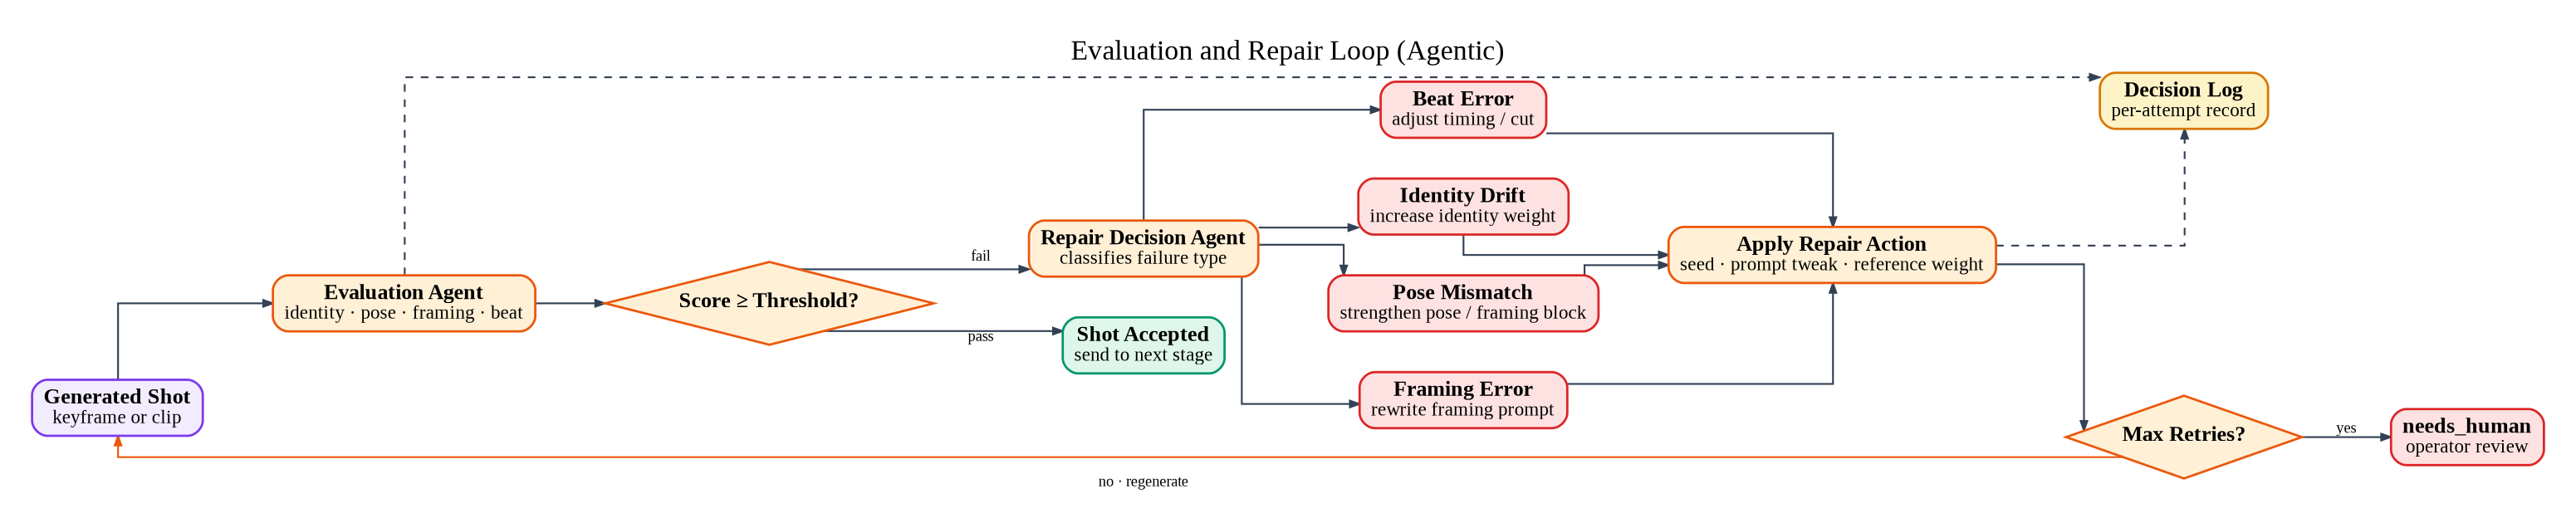
\includegraphics[width=\textwidth,height=0.85\textheight,keepaspectratio]{figs/evaluation_repair_loop_optimized.png}
\par\vspace{3pt}{\footnotesize \textbf{Figure 3.7} --- The \emph{designed} Stage-4 automatic evaluation--repair loop: the Evaluation Agent scores each shot; on pass the shot is accepted, on fail the Repair Decision Agent classifies the failure (identity drift / pose mismatch / framing error / beat error) and applies a targeted repair, logging every attempt, escalating to \texttt{needs\_human} at max retries. This is the \emph{designed} automatic loop; the executed runs (\S{}3.6.3, \S{}4.4) used a \textbf{human-gated} diagnose-and-retry loop that writes the \textbf{same decision-log schema}. The fully automatic, scoring-driven loop was not fully executed.}
\end{figure*}

\begin{figure*}[!tp]
\centering
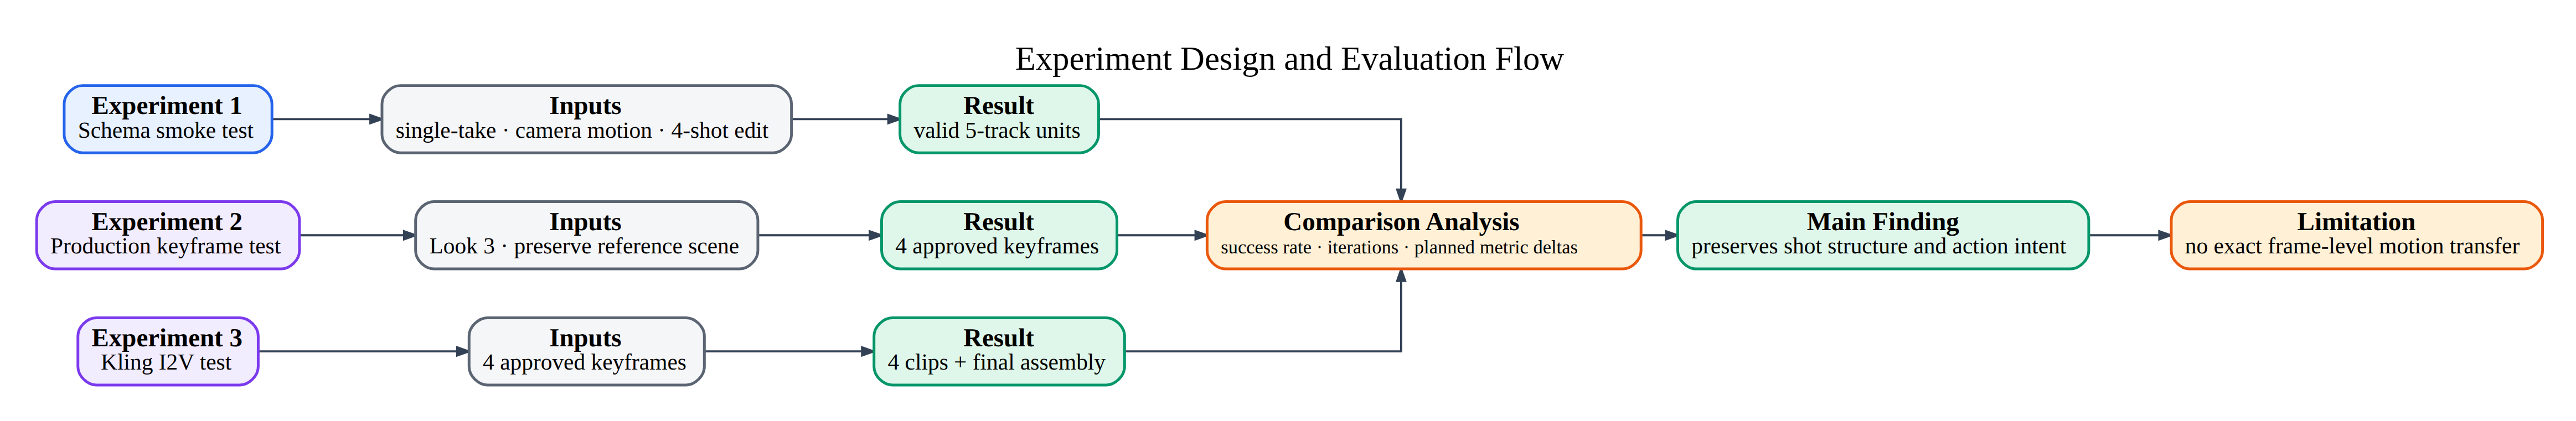
\includegraphics[width=\textwidth,height=0.85\textheight,keepaspectratio]{figs/experiment_evaluation_flow_optimized.png}
\par\vspace{3pt}{\footnotesize \textbf{Figure 3.8} --- The \emph{designed} experiment and evaluation flow. \textbf{Executed} (human visual review, \S{}4.3--\S{}4.7): the schema smoke test, per-shot keyframe generation and Kling I2V. \textbf{Planned / pending} (\S{}4.2, \S{}4.9): the automated comparison analysis --- success rate, iteration counts, metric deltas --- and the loop-off-versus-loop-on ablation are designed but not yet executed. The executed finding is that reference shot structure and action intent are preserved, within the claim boundary stated above (\S{}3.5.3).}
\end{figure*}

\addcontentsline{toc}{subsubsection}{3.6.3 Loop trigger on the reported run (honest note)}

\subsection*{3.6.3 Loop trigger on the reported run (honest note)}

On \texttt{live\_test\_03\_4shots}, the automated scoring in this section was \textbf{not yet executed}: identity (ArcFace) and pose-keypoint (DWPose) scores were not computed on this batch at generation time (an ArcFace cosine similarity was later computed as a post-hoc diagnostic, \S{}4.8.1), framing was assessed by human visual review, and the automatic repair loop was \textbf{not triggered}. The loop that \emph{did} operate on this run was the \textbf{keyframe-approval loop} --- a human-in-the-loop gate that diagnoses a failed keyframe and regenerates it before the shot is animated (\S{}3.7). The automated Stage-4 loop described above is the designed mechanism; \S{}3.9 states precisely what has and has not been run so that no evaluation claim outruns its evidence.

\addcontentsline{toc}{subsection}{3.7 Central state file and decision log}

\section*{3.7 Central state file and decision log}

The pipeline's core is not "several agents chatting" but a single readable/writable \textbf{\texttt{project\_state.json}} that every stage transitions. Its most important element for this dissertation is the \textbf{per-shot decision log}, which is the concrete evidence that the system is agentic: each shot records its attempts, and each attempt records the action taken, the outcome, and --- where applicable --- the diagnosis that motivated the next attempt.

The reference run's decision log (\texttt{decision\_log.json}, schema \texttt{decision\_log\_v1}) demonstrates this at the keyframe stage. Each shot stores the model and slot configuration, the exact prompt used, the number of attempts, the issue encountered, and the fix applied:

\begin{table*}[t]
\centering
\footnotesize
\begin{tabularx}{\textwidth}{l>{\RaggedRight\arraybackslash}X>{\RaggedRight\arraybackslash}X>{\RaggedRight\arraybackslash}X>{\RaggedRight\arraybackslash}X}
\toprule
Shot & Keyframe attempts & Issue diagnosed & Repair action & Improved? \\
\midrule
shot\_001 & 1 & --- & v3 prompt (preserve scene, over-shoulder MCU) & approved first attempt \\
shot\_002 & 2 & v1 blocked by forbidden-word guard (bridal terms in negatives) & separate positive/negative prompts; v2 natural-realism language & yes \\
shot\_003 & 2 & v1 described a face-forward pose --- wrong for the source frame & inspect source frame $\rightarrow$ v2 rewritten as extreme low-angle feet close-up & yes \\
shot\_004 & 3 & v1--v2 rendered a generic business blazer, not the specified look & v3: labelled BLAZER/TIE/TROUSERS subsections + stronger negatives + look-front to slot \texttt{[1]} & yes \\
\bottomrule
\end{tabularx}
\end{table*}

This table is a \textbf{diagnose $\rightarrow$ act $\rightarrow$ re-evaluate} trace: each retry is a decision conditioned on an observed failure, not a blind re-roll. It is exactly the shape the automated Stage-4 loop is designed to produce, executed here through the human-approval gate. The decision log therefore doubles as dissertation evaluation data, and the same schema (attempts, scores, verdict, diagnosis, repair action, terminal \texttt{needs\_human}) is the container the automated loop writes into when it runs.

\addcontentsline{toc}{subsection}{3.8 Copyright-aware workflow and Mode B}

\section*{3.8 Copyright-aware workflow and Mode B}

\textbf{Copyright.} The workflow is designed so that no protected reference content can reach the output. References are authorised, self-created or royalty-free, and are analysed only for formal structure (rhythm, shot structure, generic motion, framing). Reference \textbf{audio} is used for beat analysis only and never appears in the output. Outputs use the original IP character, new scene prompts, and royalty-free or original assets. The governing intent is \textbf{"extract structure, regenerate content,"} never a re-skinned copy of the reference --- the reference run explicitly records that no reference pixels or audio are reproduced.

\textbf{Mode B (scoped variant).} Alongside the reference-video path, the same dashboard exposes a natural-language path: story prompt + template $\rightarrow$ GPT-4o panel plan $\rightarrow$ \texttt{gpt-image-1} animated storyboard sheet $\rightarrow$ panel review $\rightarrow$ storyboard JSON $\rightarrow$ core loop. Mode B is deliberately scoped --- \textbf{animation only, single character, no photoreal, no multi-strategy analysis} --- so that it demonstrates the storyboard-JSON-to-video half of the architecture without duplicating Mode A's reference-decomposition machinery.

\begin{figure*}[!tp]
\centering
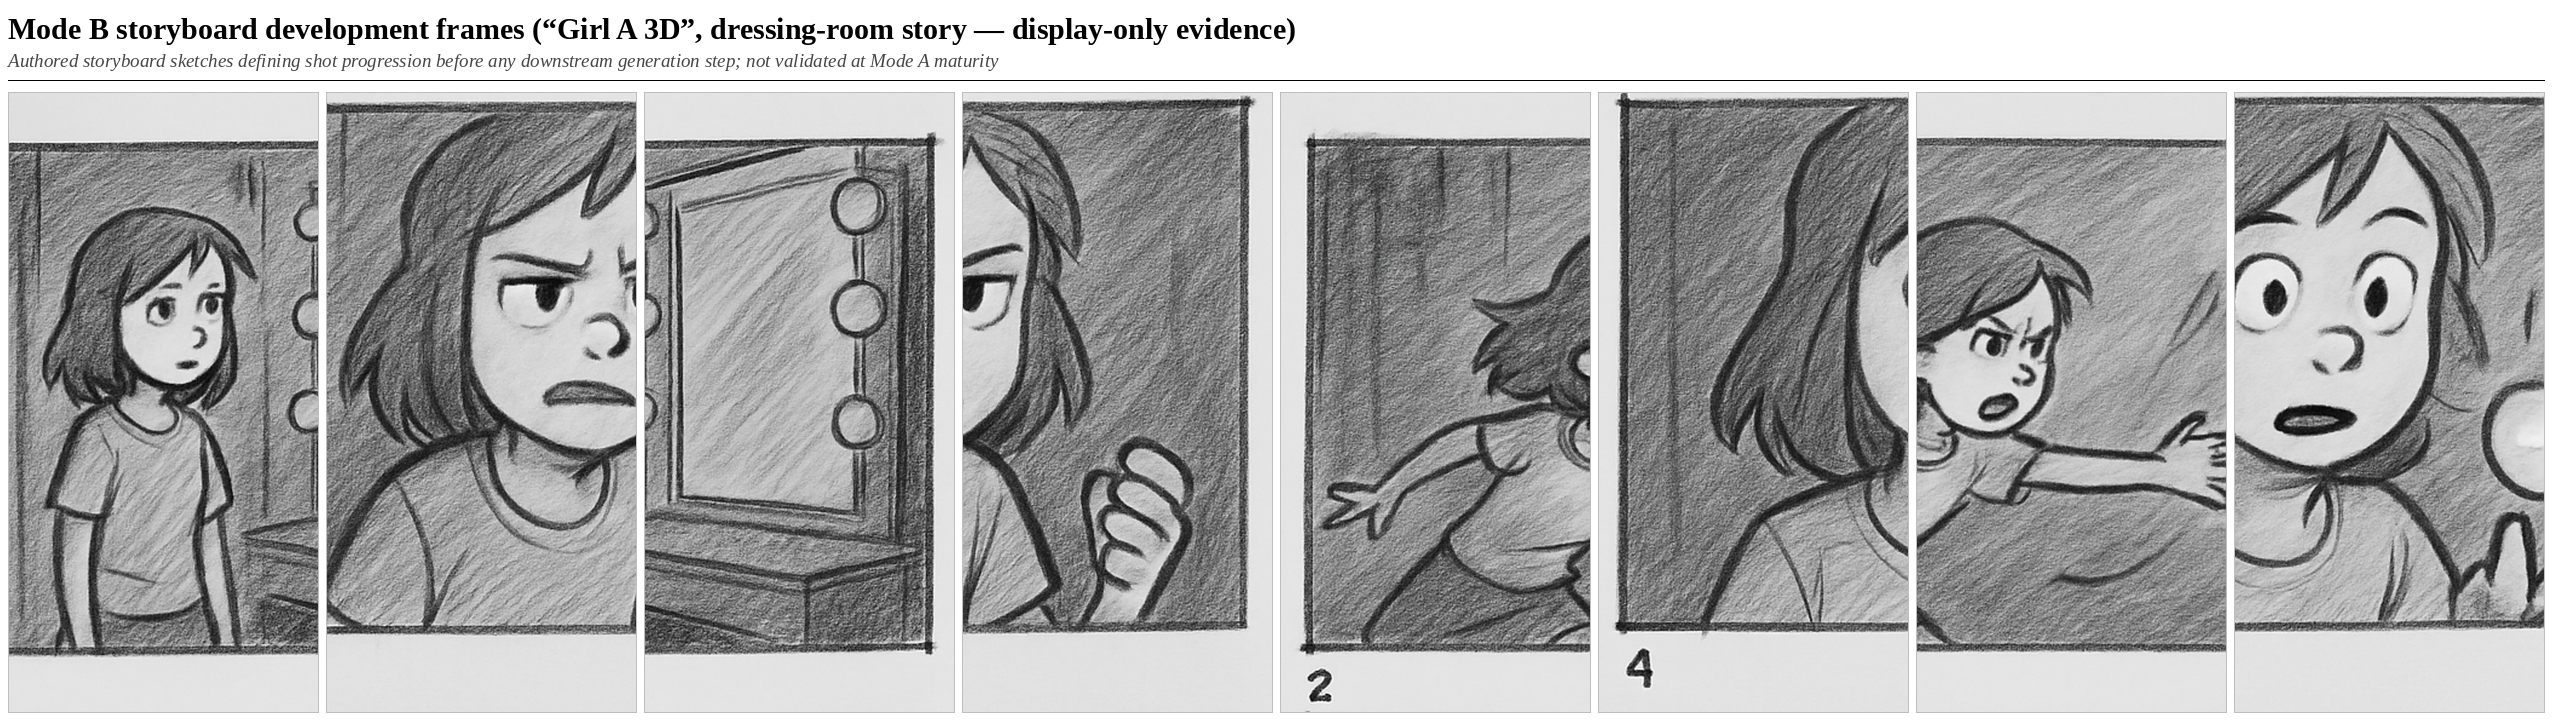
\includegraphics[width=\textwidth,height=0.85\textheight,keepaspectratio]{figs/mode_b_storyboard_contact_sheet.png}
\par\vspace{3pt}{\footnotesize \textbf{Figure 3.9} --- Mode B storyboard development frames (character look \texttt{girl\_a\_3d}, a dressing-room story; \texttt{outputs/mode\_b/panel\_plan.json}). Frames sampled from the four GPT-4o-generated storyboard panels that define shot progression before any downstream keyframe/I2V generation. This is \textbf{display-only evidence}: Mode B is not validated at the same maturity as the completed Mode A beach run (\S{}4.3--\S{}4.7), and no claim is made that it completed the full analyse--generate--evaluate--repair cycle.}
\end{figure*}

\addcontentsline{toc}{subsection}{3.9 Implementation status (what is built vs. what is designed)}

\section*{3.9 Implementation status (what is built vs. what is designed)}

To keep every downstream claim bounded, the state of each stage on the reference run is stated explicitly:

\begin{table*}[t]
\centering
\footnotesize
\begin{tabularx}{\textwidth}{>{\RaggedRight\arraybackslash}X>{\RaggedRight\arraybackslash}X>{\RaggedRight\arraybackslash}X}
\toprule
Component & Designed & Executed (status) \\
\midrule
Reference analysis (cuts/beats/motion/pose/semantic) & \ding{51} & \ding{51} --- 4 shots from 7.92 s / 123 bpm \\
Beat-aligned storyboard, five-track units & \ding{51} & \ding{51} --- all units \texttt{track\_completeness = full} \\
Keyframe-first IP-conditioned generation & \ding{51} & \ding{51} --- 4 keyframes approved \\
Kling prompt-level I2V + ffmpeg assembly & \ding{51} & \ding{51} --- 20.4 s, 768$\times$1152 final video \\
Keyframe-approval loop (human-in-the-loop, logged) & \ding{51} & \ding{51} --- decision log, 1/2/2/3 attempts \\
Automated Stage-4 scoring (ArcFace / DWPose / framing / beat) & \ding{51} & \ding{55} --- pending; not computed on this batch \\
Automated evaluation$\rightarrow$repair loop & \ding{51} & \ding{55} --- not triggered on this run \\
Start/mid/end pose sampling (Stage 1 analysis) & \ding{51} & \ding{51} --- 12 samples; pose conf/keypoints per shot \\
Graded structural guidance --- textual cues (channel 1) & \ding{51} & \ding{51} --- pose-derived cues present in per-shot prompts \\
Graded structural guidance --- skeleton reference image (channel 2) & \ding{51} & Tested, then \textbf{archived} --- implemented in the street start/end run but skeleton too weak for \texttt{gpt-image-1}; not final output (\S{}4.12) \\
Street run --- scene replacement, keyframe $\rightarrow$ I2V & \ding{51} & \ding{51} --- \texttt{live\_test\_04\_street\_look3}: 4 keyframes + 4 clips + assembled final video (human review; ArcFace pending) \\
Motion-energy audit (optical flow, street vs. reference) & \ding{51} & \ding{51} --- street clips 14--64\% of reference per-frame motion (Table 4.15) \\
Motion-prompt repair (separate appearance from motion) & \ding{51} & \ding{51} --- executed on shot\_001/003, prompt-only (no keyframe regen): 14$\rightarrow$51\%, 19$\rightarrow$47\% of reference motion (Table 4.16) \\
Mode C Condition A --- background-preserving replacement (Wan2.2-Animate) & \ding{51} (future-work extension) & \ding{51} Phase 0 only --- 480$\times$848 / 81f on RTX 4080 via Wan2GP; motion follows + background preserved; full run not validated (\S{}3.10, \S{}4.17) \\
Mode C Condition B --- full replacement + scene regeneration & \ding{51} (designed) & \ding{55} --- not yet run; no output on disk (\S{}3.10, \S{}4.17) \\
Phase 0 pose-vs-identity feasibility test & \ding{51} (planned) & \ding{55} --- not run; pipeline scoped to keyframe-first I2V \\
Loop ON vs OFF ablation (core experiment) & \ding{51} & \ding{55} --- pending automated scoring \\
\bottomrule
\end{tabularx}
\end{table*}

The foundation is valid on its own terms: a working reference-decomposition $\rightarrow$ beat-aligned storyboard $\rightarrow$ keyframe-first IP-conditioned generation $\rightarrow$ logged diagnose-and-retry loop, end to end, on a real four-shot run. The automated Stage-4 loop and its ablation are the immediate next work, and are the components whose \emph{design} --- not yet whose \emph{results} --- this chapter documents.

\addcontentsline{toc}{subsection}{3.10 Mode C --- pose-conditioned driving-video backend (two conditions)}

\section*{3.10 Mode C --- pose-conditioned driving-video backend (two conditions)}

Sections \S{}3.5.5 and (in the evaluation) \S{}4.15 repeatedly flag one direction as future work: reliable structural control needs a \textbf{pose-conditioned / driving-video backend} (Wan2.2-Animate; Cheng et al., 2025) rather than \texttt{gpt-image-1}, which follows a skeleton image only weakly. \textbf{Mode C} is a probe of exactly that direction. It is presented here as a scoped extension, not as a mode on equal footing with Mode A: the argument of this dissertation rests on Mode A, and Mode C is reported only to establish whether the flagged backend is feasible and how it behaves. Rather than treat these as two separate modes, Mode C is one backend (\textbf{Wan2.2-Animate}) with \textbf{two conditions} that differ only in what happens to the scene.

\textbf{Condition A --- background-preserving replacement.} Given a \textbf{driving performance video}, the system preserves the original background, camera and timing and replaces only the performer. Two per-frame conditioning signals are extracted from the driving video: a \textbf{DWPose skeleton} and a \textbf{SAM-style person mask} (Segment Anything family; Kirillov et al., 2023) --- see Figure 3.10. These condition Wan2.2-Animate (Replacement Mode) so the target character follows the driving motion while the background \emph{outside} the mask is preserved. Unlike Mode A's prompt-level I2V, the pose here is a genuine per-frame structural control consumed by the backend.

\begin{figure*}[!tp]
\centering
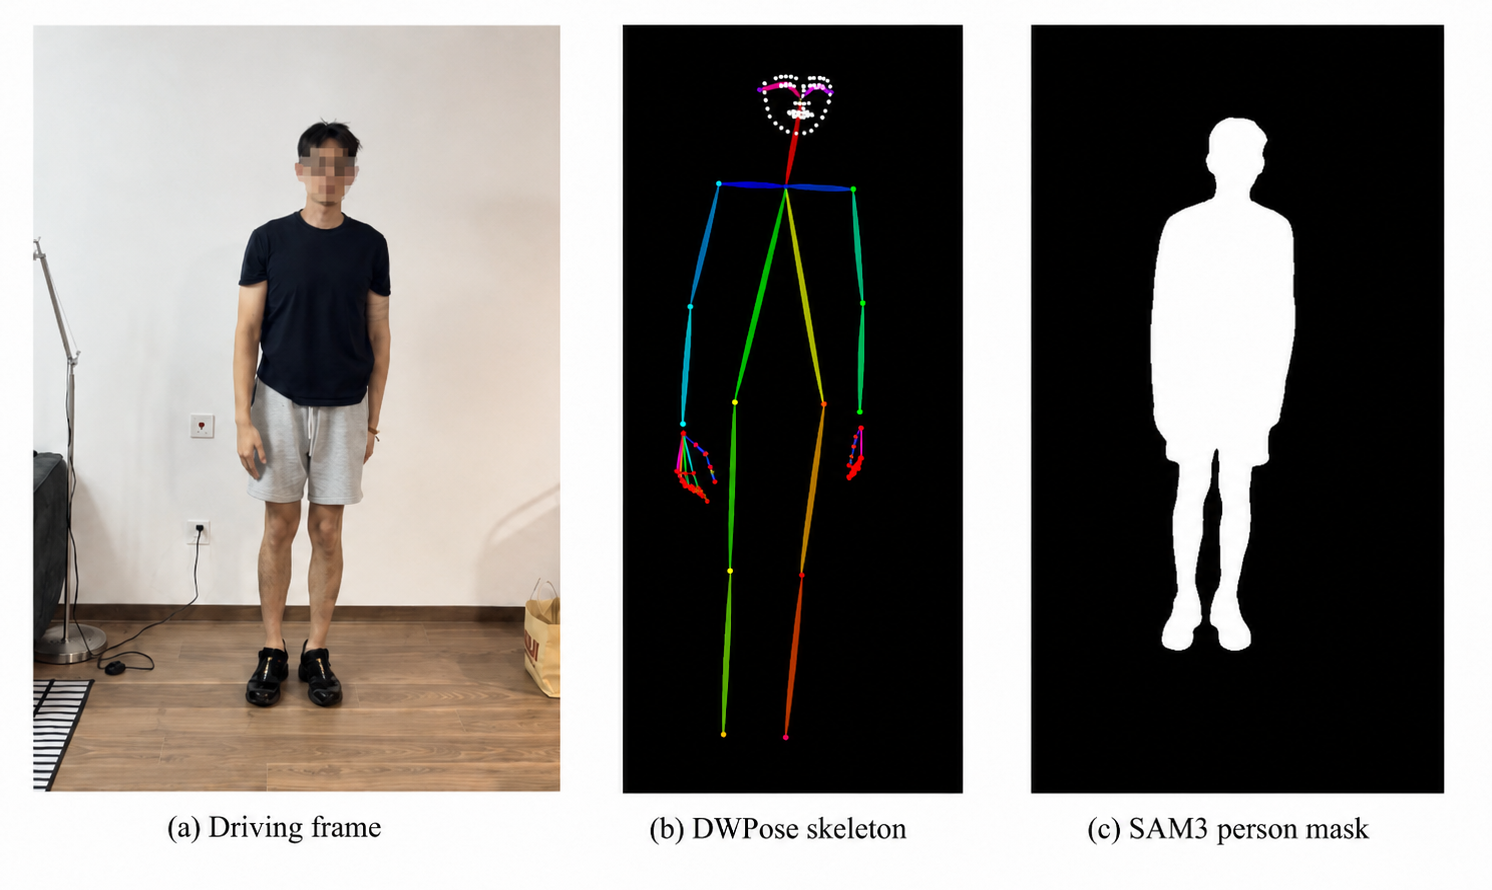
\includegraphics[width=\textwidth,height=0.85\textheight,keepaspectratio]{figs/mode_c_preprocessing.png}
\par\vspace{3pt}{\footnotesize \textbf{Figure 3.10} --- Mode C (Condition A) preprocessing. The driving performance video is decomposed into a per-frame \textbf{DWPose skeleton} and a \textbf{SAM-style person mask}; these condition the Phase 0 Mode C backend (Wan2.2-Animate replacement) so the target character follows the driving motion while the background outside the mask is preserved. The driving performer's face is anonymised (\S{}5.2). This figure shows preprocessing only; it does not depict production-quality full-video output.}
\end{figure*}

\textbf{Condition B --- full replacement / animation (planned).} The same backend can instead \textbf{regenerate the scene}: the performer is replaced \emph{and} a new environment is generated, keeping only the driving motion and the target character. Condition B therefore drops the background-preservation constraint of Condition A and is evaluated differently (\S{}4.17) --- \textbf{scene coherence} replaces background preservation, alongside the same motion-follow and identity checks. Condition B is \textbf{designed but not yet run on the local backend} (no local Condition B output exists on disk at the time of writing --- \S{}4.18 separately reports a dated, hosted-service Condition-B-style output as a supplementary comparison, not a substitute for this local run); it is reported as the backend's second condition and will become an executed local result once generated.

\textbf{Boundaries relative to Mode A (kept explicit).} Mode C uses a \textbf{different backend} (Wan2.2-Animate via Wan2GP, not \texttt{gpt-image-1} keyframes + Kling I2V), a \textbf{different character} (Look 1, matched to the workout driving video), \textbf{no} beat-aligned storyboard JSON, and is \textbf{not} keyframe-first; it also runs on a separate GPU host, not the dashboard environment. It is therefore a genuinely separate second generation backend, reported as a feasibility extension and \textbf{not integrated} into the Mode A pipeline. Its results are reported under the same reporting rule in \S{}4.17. Figure 1 (\S{}1.1) summarises how the four input modes relate: Modes A and B share the keyframe-first orchestration core with separated identity/look/scene conditioning, Mode C is the separate driving-video backend, and Mode D is a planned hosted-service extension only.

\begin{quotebox}Mode C is a Phase 0 feasibility probe of the pose-conditioned, driving-video backend flagged as future work in \S{}3.5.5 and \S{}4.15. It is not integrated into the Mode A pipeline and uses a different backend (Wan2.2-Animate via Wan2GP) and a different character; it is reported only to establish whether such a backend is feasible on available hardware and to characterise its reference-role behaviour.\end{quotebox}

\addcontentsline{toc}{subsection}{3.11 Project planning, milestones and risk management}

\section*{3.11 Project planning, milestones and risk management}

The project was planned around a single organising principle: \textbf{build the riskiest unknown first}. The standard temptation in a pipeline of this kind is to begin with the parts that are certain to work --- the deterministic analysis tools (PySceneDetect, librosa, MediaPipe) all function out of the box --- and defer the hard question. That ordering is inverted here. The central technical risk, the tension between strong pose conditioning and character-identity preservation (\S{}3.5.4), was addressed first, as a \textbf{Phase 0 feasibility test} with a pre-declared quantitative pass criterion, so that the whole build could be re-scoped early if it failed rather than after months of investment.

\addcontentsline{toc}{subsubsection}{3.11.1 Milestones}

\subsection*{3.11.1 Milestones}

The work was organised into the sequence below. Dates are indicative of the phase order and duration and were executed against the submission calendar over roughly a ten-week window in summer 2026.

\begin{table*}[t]
\centering
\footnotesize
\begin{tabularx}{\textwidth}{l>{\RaggedRight\arraybackslash}Xl}
\toprule
Phase & Milestone & Window (2026) \\
\midrule
Scoping & Problem definition, reference-driven concept, locked four-stage architecture & 7--19 Jun \\
Phase 0 & Feasibility test: IP identity vs. pose conditioning, with a pre-set pass threshold & 19--24 Jun \\
Stage 1--2 & Reference Analysis + beat-aligned storyboard (five-track units) & 25 Jun -- 2 Jul \\
Stage 3 & IP-conditioned keyframe-first generation; identity-anchor system & 2--10 Jul \\
Stage 4 & Evaluation + repair loop; decision log; end-to-end beach run & 10--19 Jul \\
Extension & Scene-replacement street run; Mode C driving-video probe & 19--28 Jul \\
Write-up & Evaluation, ethics, dissertation, submission & 28 Jul -- 10 Aug \\
\bottomrule
\end{tabularx}
\end{table*}

The build order within the milestones follows the same risk-first logic: Phase 0, then the analysis and template stages, then per-shot generation, then the automatic evaluation and repair loop, with interface and packaging deliberately last. Figure 3.11 shows the schedule as a timeline. The plan is notable for placing the highest-risk task (Phase 0) second, immediately after scoping, so that the risk to the whole approach was assessed at the start of the build and a scoped, keyframe-first fallback adopted, rather than the risk being discovered late.

\begin{figure*}[!tp]
\centering
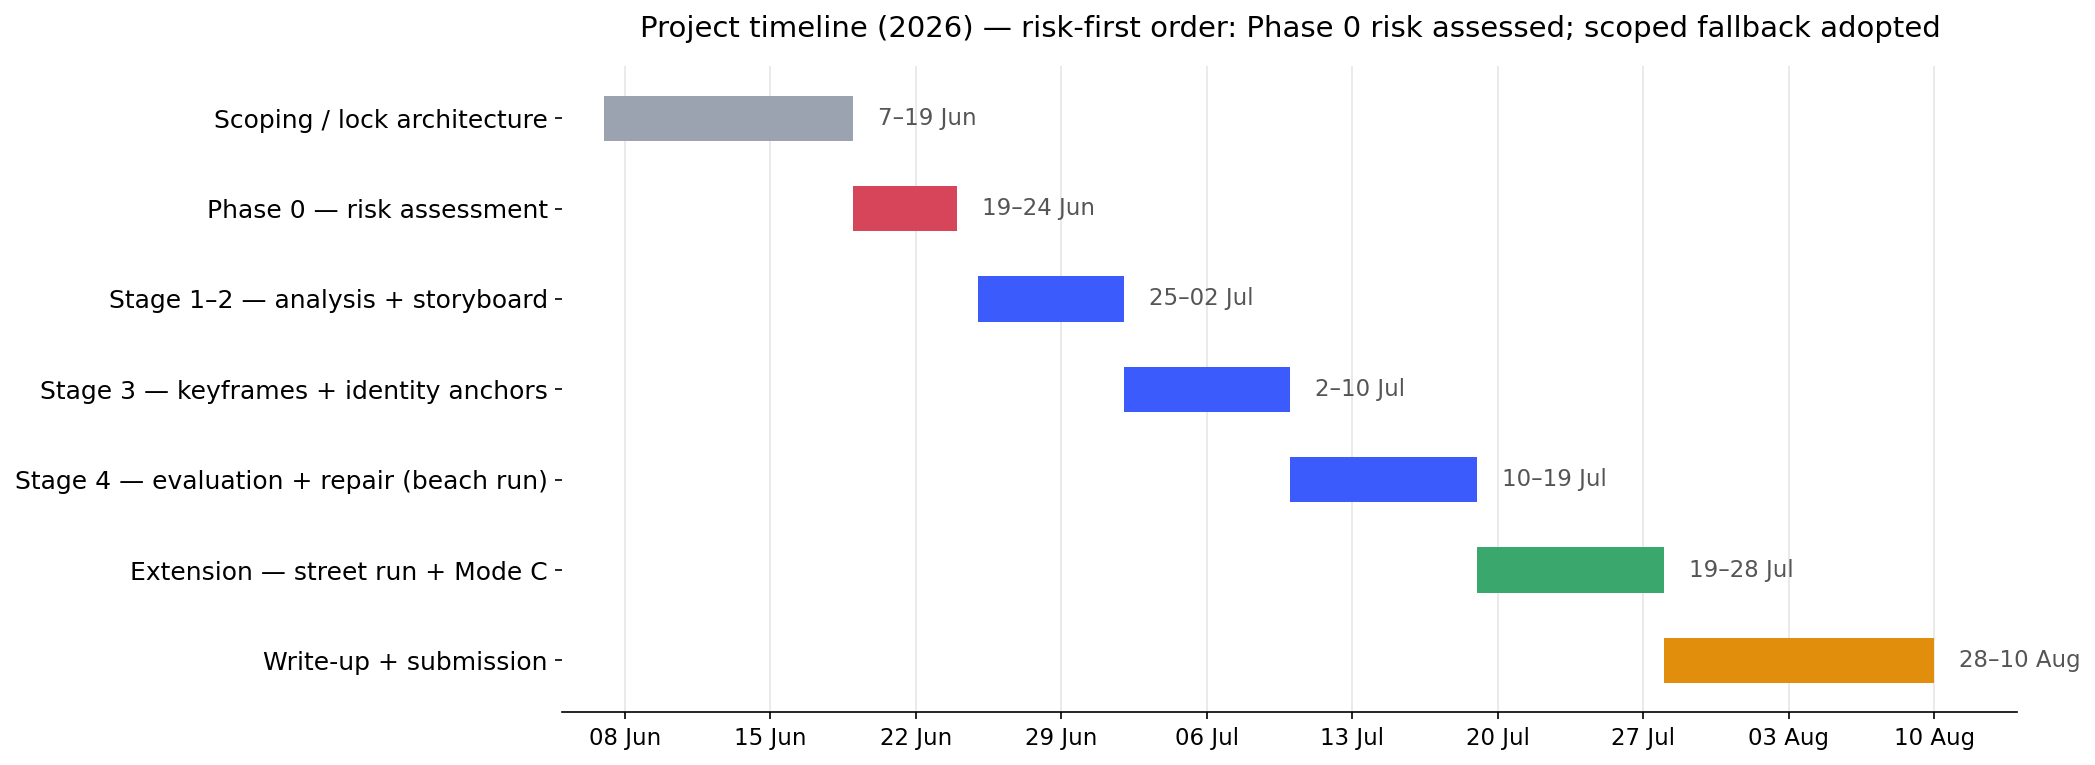
\includegraphics[width=\textwidth,height=0.85\textheight,keepaspectratio]{figs/project_timeline.png}
\par\vspace{3pt}{\footnotesize \textbf{Figure 3.11} --- Project timeline (2026). The build follows a risk-first order: the highest-risk component, the Phase 0 pose-vs-identity feasibility test, is scheduled immediately after scoping so that the risk to the whole approach is assessed early and the scoped keyframe-first fallback adopted rather than the risk being discovered late; the analysis, generation and evaluation--repair stages follow, with the scene-replacement and Mode C extensions and the write-up last.}
\end{figure*}

\addcontentsline{toc}{subsubsection}{3.11.2 Risk register and contingencies}

\subsection*{3.11.2 Risk register and contingencies}

Risk management was explicit and, in several cases, is directly visible in the results as executed decisions rather than after-the-fact rationalisation.

\begin{table*}[t]
\centering
\footnotesize
\begin{tabularx}{\textwidth}{>{\RaggedRight\arraybackslash}X>{\RaggedRight\arraybackslash}X>{\RaggedRight\arraybackslash}X>{\RaggedRight\arraybackslash}X}
\toprule
Risk & Likelihood / impact & Mitigation & Contingency (downgrade path) \\
\midrule
Pose conditioning distorts the IP identity & High / high & Phase 0 test with a quantitative pass gate before full build & \textbf{Keyframe-remake}: drop full motion transfer, deliver consistent key poses + beat-driven cuts (\S{}3.5.4) \\
Closed-API identity drift on face-visible shots & High / med & Front/profile identity anchors + reference-role separation + high input fidelity (\S{}4.12) & Human-gated acceptance; stronger identity (LoRA/InstantID) deferred to future work \\
Pose-as-image guidance too weak to control the API & Med / med & Graded structural conditioning matched to per-shot pose reliability (\S{}3.5.5) & Branch tested and \textbf{archived} as a negative result rather than forced (\S{}4.12) \\
Auto-analysis (Stage 1--2) unreliable on a given clip & Low / high & Deterministic, validated tools with a schema smoke test (\S{}4.3) & \textbf{Hand-authored storyboard JSON} keeps the downstream pipeline valid \\
Scope creep beyond an MSc timeline & Med / med & Locked architecture; start/end frames and Mode C explicitly bounded as enhancements & Cut enhancements first; the core loop is the deliverable \\
GPU / cost constraints & Med / med & Closed inference APIs + zero-cost local analysis; attempt counts tracked & Mode C limited to a Phase 0 window on available 16 GB hardware \\
\bottomrule
\end{tabularx}
\end{table*}

The two downgrade paths --- \textbf{keyframe-remake} in place of full motion transfer, and a \textbf{hand-authored storyboard} in place of auto-analysis --- were designed in from the start as deliberate scoping moves, not as failures, and are what guarantee a valid dissertation artefact under an MSc timeline regardless of how the highest-risk components resolve.

\par\vspace{22pt}
\Needspace*{12\baselineskip}
\addcontentsline{toc}{section}{Chapter 4 --- Evaluation and Results}

\vspace*{2pt}\noindent{\LARGE\bfseries Chapter 4 --- Evaluation and Results\par}\vspace{3pt}\hrule height 0.8pt\vspace{12pt}

\addcontentsline{toc}{subsection}{4.1 Aims and the meaning of "result" in this chapter}

\section*{4.1 Aims and the meaning of "result" in this chapter}

The evaluation has two jobs. First, to establish that the pipeline runs \textbf{end to end} on a real reference and produces a coherent vertical short --- the \emph{system-works} result. Second, to specify the \textbf{automated, quantitative} evaluation that measures per-shot quality (identity, pose, framing, beat) and that drives the agentic repair loop --- the \emph{system-is-good} result.

At the time of writing, the first job is \textbf{done and verified}; the second is \textbf{designed, implemented in schema, and pending execution}. This chapter is deliberate about the boundary between the two. Where a result was produced by running the pipeline, it is reported as a result. Where a measurement is designed but has not been run, it is reported as a placeholder with an explicit \texttt{pending} status. No identity, pose, framing or beat score is invented, estimated, or implied.

A single claim boundary governs every result below and should accompany any demonstration of the system:

\begin{quotebox}\textbf{The system preserves reference shot structure and action intent, but does not perform exact frame-level motion transfer.}\end{quotebox}

\addcontentsline{toc}{subsection}{4.2 Evaluation status at a glance}

\section*{4.2 Evaluation status at a glance}

Table 4.1 summarises what was executed versus what remains planned on the reference run. The detailed per-experiment results follow in \S{}4.3--\S{}4.6; the planned automated evaluation is specified in \S{}4.8--\S{}4.10.

\begin{table*}[t]
\centering
{\footnotesize\textbf{\textbf{Table 4.1 --- Executed vs. planned evaluation on \texttt{live\_test\_03\_4shots}}}}\par\vspace{3pt}
\footnotesize
\begin{tabularx}{\textwidth}{>{\RaggedRight\arraybackslash}Xl>{\RaggedRight\arraybackslash}X}
\toprule
Evaluation component & Type & Status on this run \\
\midrule
Schema smoke test (five-track unit completeness) & Executed & \ding{51} Complete \\
Keyframe generation (per-shot, human-approved) & Executed & \ding{51} 4/4 approved \\
Kling I2V clip generation & Executed & \ding{51} 4/4 succeeded \\
End-to-end assembly (final video) & Executed & \ding{51} 768$\times$1152, 20.4 s \\
Human visual review (identity/framing/look) & Executed & \ding{51} All shots approved \\
ArcFace identity scoring & Executed (post-hoc diagnostic) & \ding{51} Computed post-hoc (\S{}4.8.1) \\
Pose-keypoint (DWPose) similarity & Planned & \ding{55} Pending --- not computed \\
Framing-accuracy metric & Planned & \ding{55} Pending --- visual only \\
Beat-alignment error (ms) & Planned & \ding{55} Pending --- not computed \\
Baseline (loop OFF) vs. agentic (loop ON) ablation & Planned & \ding{55} Pending --- automated loop not run \\
\bottomrule
\end{tabularx}
\end{table*}

The verified contribution of this run is therefore an \textbf{end-to-end generation success under human visual review}; the remaining automated metric layer (pose, framing, beat) and its ablation are the next evaluation step (\S{}4.7, \S{}4.15).

Table 4.2 consolidates every result actually executed in this chapter, so the reader can see at a glance what was run versus what remains pending. Detailed evidence follows in \S{}4.3--\S{}4.13, with three former placeholders converted to measured values later in the chapter: a shot-segmentation control (\S{}4.3.1), an ArcFace identity score (\S{}4.8.1) and a log-derived loop ablation (\S{}4.9).

\begin{table*}[t]
\centering
{\footnotesize\textbf{\textbf{Table 4.2 --- Summary of executed results (this chapter).} Every row is from an execution log, \texttt{decision\_log.json}, \texttt{ffprobe}, local optical-flow / ArcFace, or human visual review. Rows marked \emph{reconstructed} are derived from the logged attempt record, not an independent re-execution. Framing-accuracy and beat-alignment automated scores are deliberately absent --- they remain pending.}}\par\vspace{3pt}
\footnotesize
\begin{tabularx}{\textwidth}{>{\RaggedRight\arraybackslash}X>{\RaggedRight\arraybackslash}X>{\RaggedRight\arraybackslash}X}
\toprule
Result & Value & Basis \\
\midrule
Shot segmentation (main clip) & 4 shots (3 cuts) & Executed (PySceneDetect) \\
Segmentation control (single-take) & 1 shot each (test\_01 / test\_02) & Executed \\
Keyframes generated \& approved & 4 / 4 (human review) & Executed \\
Total generation attempts & 8 (1/2/2/3 per shot) & Executed (decision log) \\
Final beach video & 768$\times$1152, 20.4 s & Executed (\texttt{ffprobe}) \\
Start/mid/end pose confidence & 0.47 / 0.80 / 0.00 / 0.83 & Executed (MediaPipe) \\
Motion-energy capture (street) & 14--64\% of reference & Executed (optical flow) \\
Motion repair (shot\_001 / shot\_003) & 14$\rightarrow$51\%, 19$\rightarrow$47\% & Executed (prompt-only) \\
Identity (ArcFace, face-visible) & 0.374, 0.227 (mean 0.301) & Executed (this session) \\
Loop-OFF vs Loop-ON & 25\% $\rightarrow$ 100\% accepted & Reconstructed (decision log) \\
Mode C Condition A replacement & 480$\times$848, 81 f, on 16 GB & Executed (human review) \\
Mode C full-7\,s replacement $\times$3 & 544$\times$960, 209 f, 3 windows & Executed (Wan2GP, 4 Aug) \\
\bottomrule
\end{tabularx}
\end{table*}

\addcontentsline{toc}{subsection}{4.3 Experiment 1 --- Schema smoke test}

\section*{4.3 Experiment 1 --- Schema smoke test}

\textbf{Type: Executed.} The schema smoke test checks that the reference-analysis and template-builder stages produce a structurally valid, per-shot storyboard --- i.e. that every detected shot expands into a complete five-track generation unit. This is the precondition for any downstream generation: an incomplete unit cannot be prompted or scored.

The reference clip (\texttt{test/test\_03\_multishot\_edit\_4shots.mp4} --- 7.92 s, 30 fps, 123 bpm) was decomposed into four shots, and all four produced full five-track units.

\begin{table*}[t]
\centering
{\footnotesize\textbf{\textbf{Table 4.3 --- Schema smoke test: five-track unit completeness (Executed)}}}\par\vspace{3pt}
\footnotesize
\begin{tabularx}{\textwidth}{ll>{\RaggedRight\arraybackslash}X>{\RaggedRight\arraybackslash}X>{\RaggedRight\arraybackslash}X}
\toprule
shot\_id & Duration (s) & Framing class & Camera-motion class & Track completeness \\
\midrule
shot\_001 & 2.40 & Over-shoulder MCU (medium) & push\_in & full (5/5) \\
shot\_002 & 2.27 & Wide back-view (wide) & static & full (5/5) \\
shot\_003 & 2.13 & Extreme low-angle feet CU & handheld & full (5/5) \\
shot\_004 & 1.10 & Wide side-profile (wide) & handheld & full (5/5) \\
\bottomrule
\end{tabularx}
\end{table*}

\emph{Result:} 4/4 shots reached \texttt{track\_completeness = full}. The schema pipeline is validated; the storyboard JSON is well-formed and ready for generation. No generation-quality claim is made here --- this test concerns structural validity only.

\addcontentsline{toc}{subsubsection}{4.3.1 Shot-segmentation smoke test}

\subsection*{4.3.1 Shot-segmentation smoke test}

The four-shot decomposition that all downstream evidence depends on could, in principle, be an artefact of a permissive cut threshold. To check the segmenter, Stage 1 was run on three reference clips of known structure (PySceneDetect \texttt{ContentDetector}, threshold 27): two single-take clips that should return one shot, and the multi-shot beach clip that should return four.

\begin{table*}[t]
\centering
{\footnotesize\textbf{\textbf{Table 4.4 --- Shot-segmentation smoke test (Executed; PySceneDetect \texttt{ContentDetector}, threshold 27).}}}\par\vspace{3pt}
\footnotesize
\begin{tabularx}{\textwidth}{l>{\RaggedRight\arraybackslash}Xlll}
\toprule
Reference clip & Type & Resolution & Dur. & Shots \\
\midrule
test\_01 & single-take, static camera & 1080$\times$1920 & 9.3 s & 1 \\
test\_02 & single-take, push / pan & 1920$\times$1080 & 7.8 s & 1 \\
test\_03 & multi-shot edit (main reference) & 1916$\times$1080 & 7.9 s & 4 \\
\bottomrule
\end{tabularx}
\end{table*}

\emph{Result:} the two single-take clips return zero hard cuts and fall back to a single shot; the multi-shot clip (test\_03, the beach reference used throughout) returns three cuts and four shots. This confirms the Stage 1 segmenter distinguishes single-take from cut-based footage rather than over- or under-segmenting, so the four-shot decomposition is not an artefact of a permissive threshold.

\addcontentsline{toc}{subsection}{4.4 Experiment 2 --- Keyframe generation attempts}

\section*{4.4 Experiment 2 --- Keyframe generation attempts}

\textbf{Type: Executed.} Each shot's keyframe was generated with \texttt{gpt-image-1} (\texttt{images.edit}, 1024$\times$1536, medium) conditioned on four reference images in the locked slot order (source frame, look front, look sheet, look close-up). Every candidate passed through a pre-API forbidden-word guard and a human visual review gate; rejected candidates were diagnosed and regenerated with a targeted prompt/reference revision. Table 4.5 reports the per-shot attempt history exactly as recorded in \texttt{decision\_log.json} (schema \texttt{decision\_log\_v1}).

\begin{table*}[t]
\centering
{\footnotesize\textbf{\textbf{Table 4.5 --- Keyframe generation attempts and diagnose-and-repair actions (Executed)}}}\par\vspace{3pt}
\footnotesize
\begin{tabularx}{\textwidth}{ll>{\RaggedRight\arraybackslash}X>{\RaggedRight\arraybackslash}Xl}
\toprule
shot\_id & Attempts & Diagnosed issue & Repair action taken & Final status \\
\midrule
shot\_001 & 1 & --- & v3 prompt (preserve scene, over-shoulder MCU) accepted first pass & Approved \\
shot\_002 & 2 & v1 blocked pre-API by forbidden-word guard (bridal terms in negatives) & Separated positive/negative prompt; v2 natural-realism language & Approved \\
shot\_003 & 2 & v1 prompt described a face-forward pose --- wrong for the source frame & Inspected source frame; v2 rewritten as extreme low-angle feet close-up & Approved \\
shot\_004 & 3 & v1--v2 rendered a generic business blazer, not the specified look & v3: labelled BLAZER/TIE/TROUSERS subsections, stronger negatives, look-front $\rightarrow$ slot [1] & Approved \\
\bottomrule
\end{tabularx}
\end{table*}

\emph{Result:} 4/4 keyframes approved; total 8 generation attempts across 4 shots (mean 2.0 attempts/shot). Each retry was a decision conditioned on an observed, named failure --- a \textbf{diagnose $\rightarrow$ act $\rightarrow$ re-evaluate} trace --- rather than a blind re-roll. This attempt log is the concrete evidence that the generation stage behaves agentically, executed here through the human-approval gate (see \S{}4.7 on why this is not yet the automated loop). No metric score is attached to any keyframe; approval was by human visual review.

\addcontentsline{toc}{subsection}{4.5 Experiment 3 --- Kling I2V clip results}

\section*{4.5 Experiment 3 --- Kling I2V clip results}

\textbf{Type: Executed.} Each approved keyframe was animated with Kling v1.6 (standard mode, 5 s per clip) from a natural-language video prompt describing the intended motion. All four clips were generated successfully and downloaded as MP4. Motion is \textbf{prompt-level image-to-video, not frame-level pose transfer}; no skeleton sequence, ControlNet pose map or optical-flow field was transmitted to the video model.

\begin{table*}[t]
\centering
{\footnotesize\textbf{\textbf{Table 4.6 --- Kling I2V clip results (Executed)}}}\par\vspace{3pt}
\footnotesize
\begin{tabularx}{\textwidth}{lll>{\RaggedRight\arraybackslash}X>{\RaggedRight\arraybackslash}X}
\toprule
shot\_id & Clip size (KB) & Kling status & Motion type & Intended action (video prompt, abridged) \\
\midrule
shot\_001 & 4919 & success & prompt-level I2V & Head turns back toward camera; subtle push-in \\
shot\_002 & 4347 & success & prompt-level I2V & Full-body back-view walk away toward sunset; static camera \\
shot\_003 & 7676 & success & prompt-level I2V & Low-angle feet-only walking through wet sand \\
shot\_004 & 7593 & success & prompt-level I2V & Side-profile walk toward frame-left; slight handheld \\
\bottomrule
\end{tabularx}
\end{table*}

\emph{Result:} 4/4 clips generated (100\% Kling success on approved keyframes). Action \emph{intent} is visible and consistent with each prompt; exact gait, stride length and inter-frame body position are not controlled and are not claimed. A timing caveat is noted for transparency: Kling clips are a fixed 5 s each, so per-shot \textbf{output} durations ($\approx$5 s) do not match the reference shot durations (1.10--2.40 s). Output-level beat alignment is therefore \textbf{not} achieved by this run and is part of the pending evaluation (\S{}4.8, \S{}4.15); the beat grid was used at the storyboard stage only. Motion \emph{naturalness} --- distinct from successful generation --- is measured separately in the motion-energy audit of \S{}4.13.

\addcontentsline{toc}{subsection}{4.6 End-to-end assembly result}

\section*{4.6 End-to-end assembly result}

\textbf{Type: Executed.} The four clips were concatenated with \texttt{ffmpeg} (stream copy, no re-encode) into the final vertical short. \texttt{ffprobe} confirms the delivered file:

\begin{table*}[t]
\centering
{\footnotesize\textbf{\textbf{Table 4.7 --- Final assembled video (Executed, \texttt{ffprobe}-confirmed)}}}\par\vspace{3pt}
\footnotesize
\begin{tabularx}{\textwidth}{l>{\RaggedRight\arraybackslash}X}
\toprule
Property & Value \\
\midrule
File & \texttt{final/final\_look3\_reference\_driven\_demo.mp4} \\
Resolution & 768 $\times$ 1152 (vertical, 2:3) \\
Frame rate & 30 fps \\
Duration & 20.40 s (612 frames) \\
File size & \textasciitilde{}24 MB \\
Assembly & ffmpeg concat / copy (no re-encode) \\
\bottomrule
\end{tabularx}
\end{table*}

\emph{Result:} the pipeline completes end to end --- reference decomposition $\rightarrow$ storyboard JSON $\rightarrow$ keyframe generation $\rightarrow$ I2V $\rightarrow$ assembly --- producing a single coherent 768$\times$1152 vertical short with the IP character rendered in a consistent Look 3 across four shots in a preserved beach-sunset scene. (Note: the project's stated target format is 9:16; the delivered pixels are 2:3, because \texttt{gpt-image-1}'s portrait size is 1024$\times$1536. This format gap is recorded in \S{}4.15.)

\addcontentsline{toc}{subsection}{4.7 Verified result: human visual review + successful end-to-end generation}

\section*{4.7 Verified result: human visual review + successful end-to-end generation}

This section states plainly what has and has not been demonstrated, because the distinction is the backbone of the whole evaluation.

\textbf{What is verified now.} The system produces a complete, coherent short-form video from a reference video plus a fixed IP character and a new scene, end to end, on a real four-shot run. Cross-shot \textbf{identity consistency, look fidelity and framing} were confirmed by \textbf{human visual review}, and the generation stage demonstrably repairs its own failures through a logged diagnose-and-retry loop (Table 4.5): three of the four shots required at least one corrective regeneration and all four ultimately passed review. This is a genuine result --- a working reference-driven, IP-conditioned, self-correcting generation pipeline --- and it is defensible on its own terms.

\textbf{What is not yet verified.} The review that gated this run was \textbf{human and qualitative}, not \textbf{automated and quantitative}. During generation the system did not attach automated metric scores to any shot: no ArcFace identity score, DWPose pose-similarity score, framing-accuracy value or beat-alignment error was computed in-loop, and the automatic evaluation$\rightarrow$repair loop (which consumes those scores) was \textbf{not triggered} on this run. ArcFace identity similarity was later computed as a \textbf{post-hoc diagnostic} (\S{}4.8.1); DWPose pose similarity, formal framing accuracy and beat-alignment error remain pending. Consequently the diagnose-and-retry behaviour observed here was driven by a human approving or rejecting each keyframe, not by the automated Evaluator and Repair Decision agents.

\textbf{The next evaluation step} is to run the remaining automated metrics on this exact batch, populate the remaining placeholders in \S{}4.8, and then execute the baseline-vs-agentic ablation in \S{}4.9. This converts the current \emph{system-works} result into a measured \emph{system-is-good} result without changing the pipeline.

\addcontentsline{toc}{subsection}{4.8 Evaluation metrics: post-hoc identity diagnostic and pending scores}

\section*{4.8 Evaluation metrics: post-hoc identity diagnostic and pending scores}

\begin{quotebox}
\textbf{Type:} mixed --- post-hoc diagnostic (executed) + in-loop automated scoring (planned, not executed). \quad \textbf{Input:} approved keyframes/clips from \texttt{live\_test\_03\_4shots}; ArcFace \texttt{buffalo\_l} embeddings (\S{}4.8.1). \quad \textbf{Output:} one post-hoc identity-similarity score per face-visible shot (\S{}4.8.1); pose/framing/beat cells remain \texttt{PENDING}. \quad \textbf{Proves:} a face-embedding metric can be computed post-hoc on the executed run's outputs. \quad \textbf{Does not prove:} that an in-loop, metric-driven acceptance gate ever ran on this batch --- it did not.
\end{quotebox}

\textbf{Type: Planned.} The four per-shot metrics are defined and implemented in schema but were not computed on \texttt{live\_test\_03\_4shots}. Table 4.8 fixes the metric definitions and the shape of the results table; every cell is a placeholder. \textbf{These are not results and contain no numbers.}

\begin{table*}[t]
\centering
{\footnotesize\textbf{\textbf{Table 4.8 --- Automated evaluation metrics (Planned; all cells PENDING)}}}\par\vspace{3pt}
\scriptsize
\begin{tabularx}{\textwidth}{l>{\RaggedRight\arraybackslash}X>{\RaggedRight\arraybackslash}X>{\RaggedRight\arraybackslash}X>{\RaggedRight\arraybackslash}X>{\RaggedRight\arraybackslash}X}
\toprule
shot\_id & Identity (ArcFace cosine sim.) & Pose similarity (DWPose keypoint dist.) & Framing accuracy & Beat-alignment error (ms) & Verdict ($\ge$ threshold?) \\
\midrule
shot\_001 & \emph{pending} & \emph{pending} & \emph{pending} & \emph{pending} & \emph{pending} \\
shot\_002 & \emph{pending} & \emph{pending} & \emph{pending} & \emph{pending} & \emph{pending} \\
shot\_003 & \emph{pending} & \emph{pending} & \emph{pending} & \emph{pending} & \emph{pending} \\
shot\_004 & \emph{pending} & \emph{pending} & \emph{pending} & \emph{pending} & \emph{pending} \\
\bottomrule
\end{tabularx}
\end{table*}

Metric definitions (to be applied when scoring is run):

\begin{itemize}[leftmargin=1.2em,itemsep=2pt,topsep=2pt]

\item \textbf{Identity} --- ArcFace (Deng et al., 2019) cosine similarity between the generated shot and the IP reference; higher is better. A calibrated pass threshold is to be fixed \emph{before} scoring, not chosen post hoc.

\item \textbf{Pose similarity} --- DWPose (Yang et al., 2023) keypoint distance between the generated keyframe and the reference source-frame pose; lower is closer to the reference structure. Requires DWPose extraction on the generated keyframes, which has not been run on this batch.

\item \textbf{Framing accuracy} --- match between the generated shot's composition/shot-size and the reference framing class; currently assessed visually, to be formalised.

\item \textbf{Beat-alignment error} --- millisecond distance between a cut and its nearest audio beat, under the maximum-snap-distance rule (cuts beyond the threshold are left unsnapped and reported as such).

\end{itemize}

Two run-level metrics accompany the per-shot table when scoring is run: \textbf{regeneration success rate} (fraction of failing shots repaired within the retry budget) and \textbf{number of manual interventions} (\texttt{needs\_human} escalations). Of these four metrics the \textbf{identity} score has now been computed (\S{}4.8.1); framing accuracy and beat-alignment remain pending, and pose-similarity awaits DWPose on the generated keyframes.

\addcontentsline{toc}{subsubsection}{4.8.1 Identity scoring --- executed (ArcFace)}

\subsection*{4.8.1 Identity scoring --- executed (ArcFace)}

The identity metric left pending above was computed locally with \textbf{InsightFace \texttt{buffalo\_l}} (InsightFace contributors, 2026; the \texttt{w600k\_r50} recognition model; weights fetched from the \texttt{immich-app/buffalo\_l} mirror), as the cosine similarity between each approved beach keyframe and the front Look 3 reference (\texttt{look3\_01}, a clean frontal anchor). Detection and recognition ran on CPU at zero API cost.

\begin{table*}[t]
\centering
{\footnotesize\textbf{\textbf{Table 4.9 --- Identity consistency (Executed; ArcFace \texttt{buffalo\_l} cosine to the Look 3 front anchor).}}}\par\vspace{3pt}
\footnotesize
\begin{tabularx}{\textwidth}{>{\RaggedRight\arraybackslash}X>{\RaggedRight\arraybackslash}Xl}
\toprule
Shot & Shot type & ArcFace cosine \\
\midrule
shot\_001 & face medium / turn-to-camera & 0.374 \\
shot\_002 & back-view walk & n/a (no face) \\
shot\_003 & feet-only insert & n/a (no face) \\
shot\_004 & side-profile walk & 0.227 \\
Mean over face-visible shots & --- & 0.301 \\
\bottomrule
\end{tabularx}
\end{table*}

Two shots (shot\_002 back-view, shot\_003 feet-only) contain no reliable face and are scored \texttt{not\_applicable} rather than forced to a spurious low value --- exactly the failure cases anticipated in \S{}4.15.1. The two face-visible shots score cosine similarities of 0.374 and 0.227 (mean 0.301), yet \textbf{all four frames were accepted at human review as the same Look 3 character}. This is not a contradiction to explain away: it is direct empirical confirmation of the caution in \S{}4.15.1 (point 6) --- a single face-embedding metric is mis-calibrated for a \emph{synthetic, stylised} IP character rendered under varying pose, lighting and framing, and under-scores an identity a human reader matches immediately. The low profile similarity (0.227, shot\_004) is consistent with ArcFace's known instability on non-frontal faces. This is precisely why the pipeline gates on \textbf{human review} and treats ArcFace as one operational proxy, not the arbiter. Reporting the executed number, rather than leaving it pending, converts an assumption into evidence. (Values as recorded in \texttt{project\_state.json}; independently recomputed from the keyframes for this dissertation, agreeing to within rounding.)

\addcontentsline{toc}{subsection}{4.9 Repair-loop comparison: log reconstruction and planned controlled ablation}

\section*{4.9 Repair-loop comparison: log reconstruction and planned controlled ablation}

\begin{quotebox}
\textbf{Type:} log-reconstructed observation (executed) + controlled automated ablation (planned, not executed). \quad \textbf{Input:} the \texttt{decision\_log.json} attempt history from the human-gated keyframe-approval loop (\S{}3.6.3). \quad \textbf{Output:} a reconstructed Loop-OFF-vs-Loop-ON acceptance comparison, 25\%$\rightarrow$100\% (Table 4.11). \quad \textbf{Proves:} the logged retries are diagnosed repairs, not blind re-rolls. \quad \textbf{Does not prove:} a causal, equal-budget effect size --- this is not an independently re-run controlled experiment.
\end{quotebox}

\textbf{Type: Log-reconstructed observation; controlled automated ablation planned.} The planned experiment is an automated ablation of the loop itself --- \textbf{OFF} (one-shot generation, no re-evaluation) versus \textbf{ON} (automated scoring $\rightarrow$ diagnosis $\rightarrow$ targeted regeneration) on the \S{}4.8 metrics plus regeneration success rate and manual-intervention count. It was not executed; Table 4.10 fixes the comparison design with pending outcome cells.

\begin{table*}[t]
\centering
{\footnotesize\textbf{\textbf{Table 4.10 --- Baseline (loop OFF) vs. agentic (loop ON): comparison design (Planned; outcomes PENDING)}}}\par\vspace{3pt}
\footnotesize
\begin{tabularx}{\textwidth}{>{\RaggedRight\arraybackslash}X>{\RaggedRight\arraybackslash}X>{\RaggedRight\arraybackslash}X}
\toprule
Dimension & Baseline --- loop OFF (one-shot) & Agentic --- loop ON (auto-detect + repair) \\
\midrule
Failure detection & none (accept first output) & automated scoring vs. thresholds \\
Repair & none & targeted regeneration of failing shot only \\
Identity / pose / framing / beat scores & \emph{pending} & \emph{pending} \\
Regeneration success rate & \emph{pending} & \emph{pending} \\
Manual interventions (\texttt{needs\_human}) & \emph{pending} & \emph{pending} \\
Per-shot re-generations & 0 by construction & \emph{pending} \\
\bottomrule
\end{tabularx}
\end{table*}

However, the decision log allows a conservative reconstruction, reported as \textbf{counts of approvals and attempts}, not metric scores: Loop OFF counts only each shot's first attempt; Loop ON counts the human-gated diagnose-and-retry process that actually ran (Table 4.5). This is a log-reconstructed observation, not the automated ablation of Table 4.10.

\begin{table*}[t]
\centering
{\footnotesize\textbf{\textbf{Table 4.11 --- Loop-OFF vs Loop-ON, reconstructed from the decision log (not an independent re-execution).}}}\par\vspace{3pt}
\footnotesize
\begin{tabularx}{\textwidth}{>{\RaggedRight\arraybackslash}Xl>{\RaggedRight\arraybackslash}X}
\toprule
Condition & Shots accepted & Accepted rate (human review) \\
\midrule
Loop OFF (first attempt only) & 1 / 4 & 25\% \\
Loop ON (gated repair) & 4 / 4 & 100\% \\
\bottomrule
\end{tabularx}
\end{table*}

Under Loop-OFF, only shot\_001 passes review; shot\_002--004 each required two to three gated repair attempts. Under Loop-ON --- the process actually executed --- all four shots were accepted across eight total attempts. This is not an independent equal-budget ablation and contains no metric scores; a controlled comparison with a matched attempt budget and a blind reviewer remains future work (Table 4.17). With that boundary, the log shows the value of diagnose-and-retry logging in practice: first-attempt acceptance moved from 25\% to 100\%.

\addcontentsline{toc}{subsection}{4.10 Automated scoring status for \texttt{live\_test\_03\_4shots}}

\section*{4.10 Automated scoring status for \texttt{live\_test\_03\_4shots}}

To leave no ambiguity: on the reference run reported in this chapter, \textbf{in-loop automated metric scoring is PENDING}. No automated score was attached during generation: DWPose pose-similarity, framing-accuracy and beat-alignment values were \textbf{not computed}; the automatic evaluation$\rightarrow$repair loop was \textbf{not triggered}; and the loop OFF-vs-ON ablation was \textbf{not executed} as a controlled experiment (a log-based reconstruction is reported in \S{}4.9). Only the ArcFace identity diagnostic has been computed post-hoc (\S{}4.8.1); the full in-loop automated metric layer was not executed. All results reported as \emph{Executed} in this chapter rest on pipeline execution logs, the \texttt{decision\_log.json} attempt history, \texttt{ffprobe} output, local optical-flow / ArcFace computation, and human visual review.

\addcontentsline{toc}{subsection}{4.11 Reference pose-extraction quality and graded structural guidance}

\section*{4.11 Reference pose-extraction quality and graded structural guidance}

\textbf{Type: Executed (reference analysis).} As described in \S{}3.3.1, MediaPipe Pose was run on the start, middle and end frame of each reference shot, recording pose confidence and keypoint count. This is a \textbf{reference-analysis} result on the beach reference video; it is a separate, local analysis and did \textbf{not} modify \texttt{project\_state.json} or drive the completed beach-run generation (which remained prompt-level, \S{}4.5).

\begin{figure*}[!tp]
\centering
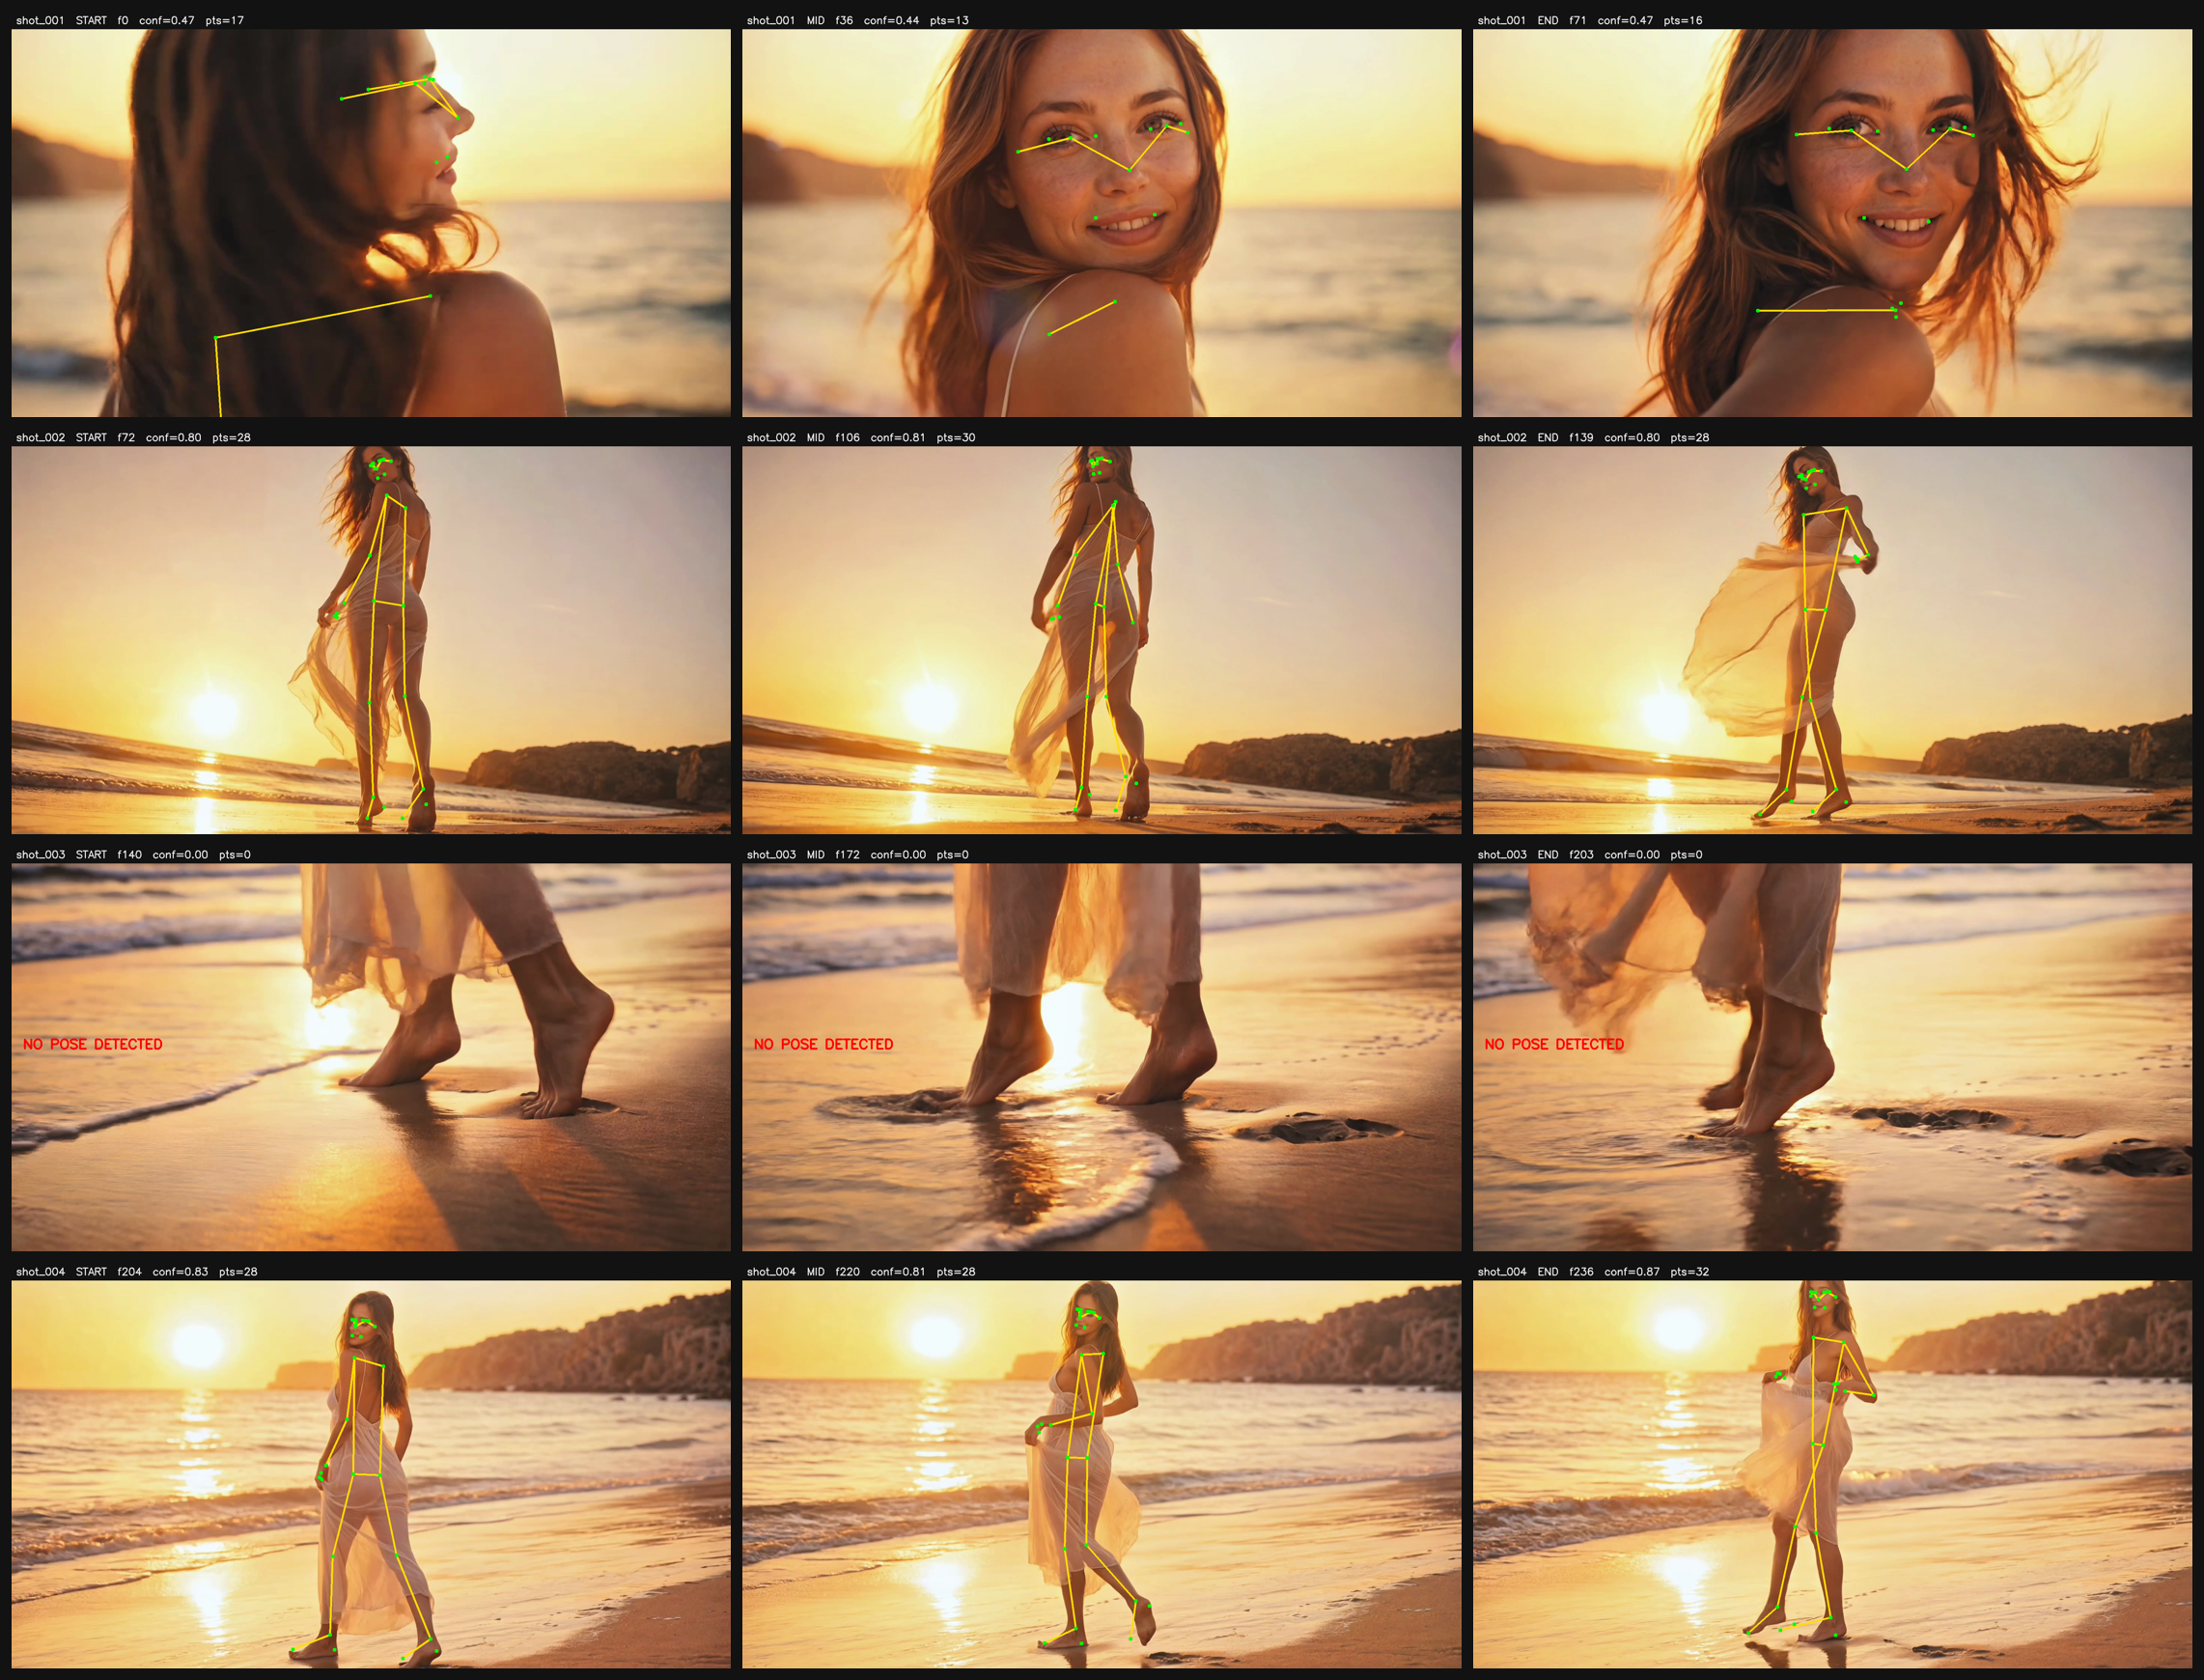
\includegraphics[width=\textwidth,height=0.85\textheight,keepaspectratio]{figs/start_mid_end_pose_extraction.png}
\par\vspace{3pt}{\footnotesize \textbf{Figure 4.1} --- Start--middle--end pose extraction from the four-shot reference video. Each row is one detected shot; each column shows the start, middle and end frame with MediaPipe pose overlays and the measured confidence / keypoint count. Pose reliability varies by shot type: full-body walking shots (shot\_002, shot\_004) yield usable skeletons, the over-shoulder close-up (shot\_001) yields sparse face/shoulder landmarks, and the feet-only insert (shot\_003) yields no detection.}
\end{figure*}

\begin{table*}[t]
\centering
{\footnotesize\textbf{\textbf{Table 4.12 --- Start/mid/end pose extraction on the reference video (Executed; local analysis)}}}\par\vspace{3pt}
\scriptsize
\begin{tabularx}{\textwidth}{l>{\RaggedRight\arraybackslash}X>{\RaggedRight\arraybackslash}Xll>{\RaggedRight\arraybackslash}X}
\toprule
shot\_id & Framing & Start conf / pts & Mid conf / pts & End conf / pts & Pose quality \\
\midrule
shot\_001 & Over-shoulder close-up & 0.47 / 17 & 0.44 / 13 & 0.47 / 16 & Sparse (face/shoulder) \\
shot\_002 & Full-body back-view walk & 0.80 / 28 & 0.81 / 30 & 0.80 / 28 & Reliable full-body \\
shot\_003 & Low-angle feet insert & 0.00 / 0 & 0.00 / 0 & 0.00 / 0 & No pose detected \\
shot\_004 & Side-profile walk & 0.83 / 28 & 0.81 / 28 & 0.87 / 32 & Reliable full-body \\
\bottomrule
\end{tabularx}
\end{table*}

Pose reliability is strongly shot-type dependent: full-body walking shots (shot\_002, shot\_004) yield stable skeletons of \textasciitilde{}28--32 keypoints at confidence $\approx$0.80--0.87 across all three sampled frames; the over-shoulder close-up (shot\_001) yields only sparse face/shoulder landmarks (13--17 keypoints, confidence $\approx$0.44--0.47) because the frame crops out the body; and the feet-only insert (shot\_003) yields \textbf{no pose at all} (0 keypoints, confidence 0.00) in every frame.

Per-shot reading:

\begin{itemize}[leftmargin=1.2em,itemsep=2pt,topsep=2pt]

\item \textbf{shot\_001 --- orientation driven.} The body skeleton is incomplete, but the useful signal is the head-orientation change across start$\rightarrow$mid$\rightarrow$end (from a partial side/back view toward a clearer over-shoulder gaze). Guided by orientation cues, not a full-body skeleton.

\item \textbf{shot\_002 --- strong structural guidance.} A stable full-body skeleton captures body placement, leg position and walking direction; eligible for the strongest structural channel.

\item \textbf{shot\_003 --- framing/text only.} No usable pose; handled through framing and textual detail (low camera angle, trouser hem, oxford shoes, cobblestone, step contact). A pose-detection failure here is not a system failure --- it is information that selects a weaker conditioning mode.

\item \textbf{shot\_004 --- strong structural guidance.} A clear, high-confidence side-profile skeleton supplies both body orientation and leg movement; unlike shot\_001 it provides full-body structure.

\end{itemize}

These readings define the \textbf{graded structural-guidance} policy of \S{}3.5.5, summarised in Table 4.13.

\begin{table*}[t]
\centering
{\footnotesize\textbf{\textbf{Table 4.13 --- Graded structural-guidance strategy from start/mid/end pose quality}}}\par\vspace{3pt}
\footnotesize
\begin{tabularx}{\textwidth}{l>{\RaggedRight\arraybackslash}X>{\RaggedRight\arraybackslash}X>{\RaggedRight\arraybackslash}X}
\toprule
Shot & Pose quality & Useful signal & Assigned conditioning mode \\
\midrule
shot\_001 & Sparse pose & Head / shoulder orientation & Orientation-cue (weak structural) \\
shot\_002 & Reliable full-body & Walking body pose and direction & Structure-guided (strong) \\
shot\_003 & No pose detected & Feet framing, ground contact & Framing/text only \\
shot\_004 & Reliable full-body & Side-profile walking pose & Structure-guided (strong) \\
\bottomrule
\end{tabularx}
\end{table*}

\emph{Result and honest boundary.} The contribution here is a \textbf{decision procedure}, not a motion-transfer result: the system measures pose reliability and assigns a per-shot conditioning strength rather than forcing unreliable pose data into every shot ("tools compute, agents decide"). The boundary is one of scope, not of feasibility. This extraction did \textbf{not} condition the completed \emph{beach} run (which used pose-derived textual cues only); it \textbf{does} drive the \emph{street start/end extension} of \S{}4.12, where the reliable shots' keypoints are rendered into neutral skeleton images and passed to keyframe generation. What is not claimed is exact motion transfer: the guidance is soft, and at the I2V stage it is absent.

\addcontentsline{toc}{subsubsection}{4.11.1 Reference-control pose/mask audit (documented control-signal trial)}

\subsection*{4.11.1 Reference-control pose/mask audit (documented control-signal trial)}

\textbf{Type: Executed (local analysis; post-hoc documented trial; no generation-API calls).} During development, reference-control extraction was explored as a possible route for stronger motion and subject-structure guidance. A documented local audit of these signals was subsequently produced for the four-shot beach reference sequence. For each shot, start, middle and end samples were inspected, giving 12 samples in total. Existing MediaPipe pose outputs (\S{}4.11) were reused, and pose-seeded OpenCV GrabCut (Bradski, 2000; Rother et al., 2004) was used to generate candidate foreground masks. Nine samples produced pose detections and mask candidates. Shot\_003, a feet-detail shot, produced no reliable pose detection across all three samples and was marked \texttt{unavailable\_no\_pose\_seed}. The per-sample pose confidences mirror the grading of \S{}4.11: the full-body shots (shot\_002, shot\_004) detect at confidence $\ge$0.80 with near-complete keypoint sets, while the close-up shot\_001 detects at 0.44--0.47 with a partial upper-body keypoint set. The audit package is hash-manifested (SHA-256) with per-file integrity verification, and was produced entirely locally at zero generation-API cost.

The audit shows that pose/mask signals are useful as \textbf{analysis and candidate-control signals}, especially for full-body shots. However, reliability varies by shot type: close-up framing and feet-detail shots were weaker, and the mask candidates were \textbf{not} treated as production-ready hard controls. This supports the final Mode~A design choice: approved keyframes, prompt-level I2V, motion-prompt repair and human-gated decision logging are used for the final evidence, rather than claiming exact skeleton-driven or alpha/mask-driven motion transfer, within the claim boundary stated in \S{}3.5.3.

\begin{table*}[t]
\centering
{\footnotesize\textbf{\textbf{Table 4.14 --- Reference-control pose/mask audit: trials, evidence and design decisions (Executed; local, post-hoc diagnostic).}}}\par\vspace{3pt}
\footnotesize
\begin{tabularx}{\textwidth}{l>{\RaggedRight\arraybackslash}X>{\RaggedRight\arraybackslash}X>{\RaggedRight\arraybackslash}X}
\toprule
Trial & Evidence & Result & Design decision \\
\midrule
Pose extraction & 12 start/mid/end samples; MediaPipe pose outputs & 9/12 usable; shot\_003 unavailable & Use as diagnostic / candidate control only \\
Mask extraction & Pose-seeded OpenCV GrabCut mask candidates & Usable mainly for full-body shots; weaker on close-up / feet shots & Not used as final hard production control \\
Final Mode A path & Approved keyframes + prompt-level I2V + repair log & More reliable for current scope & Exact frame-level motion transfer remains future work \\
\bottomrule
\end{tabularx}
\end{table*}

\begin{figure*}[!tp]
\centering
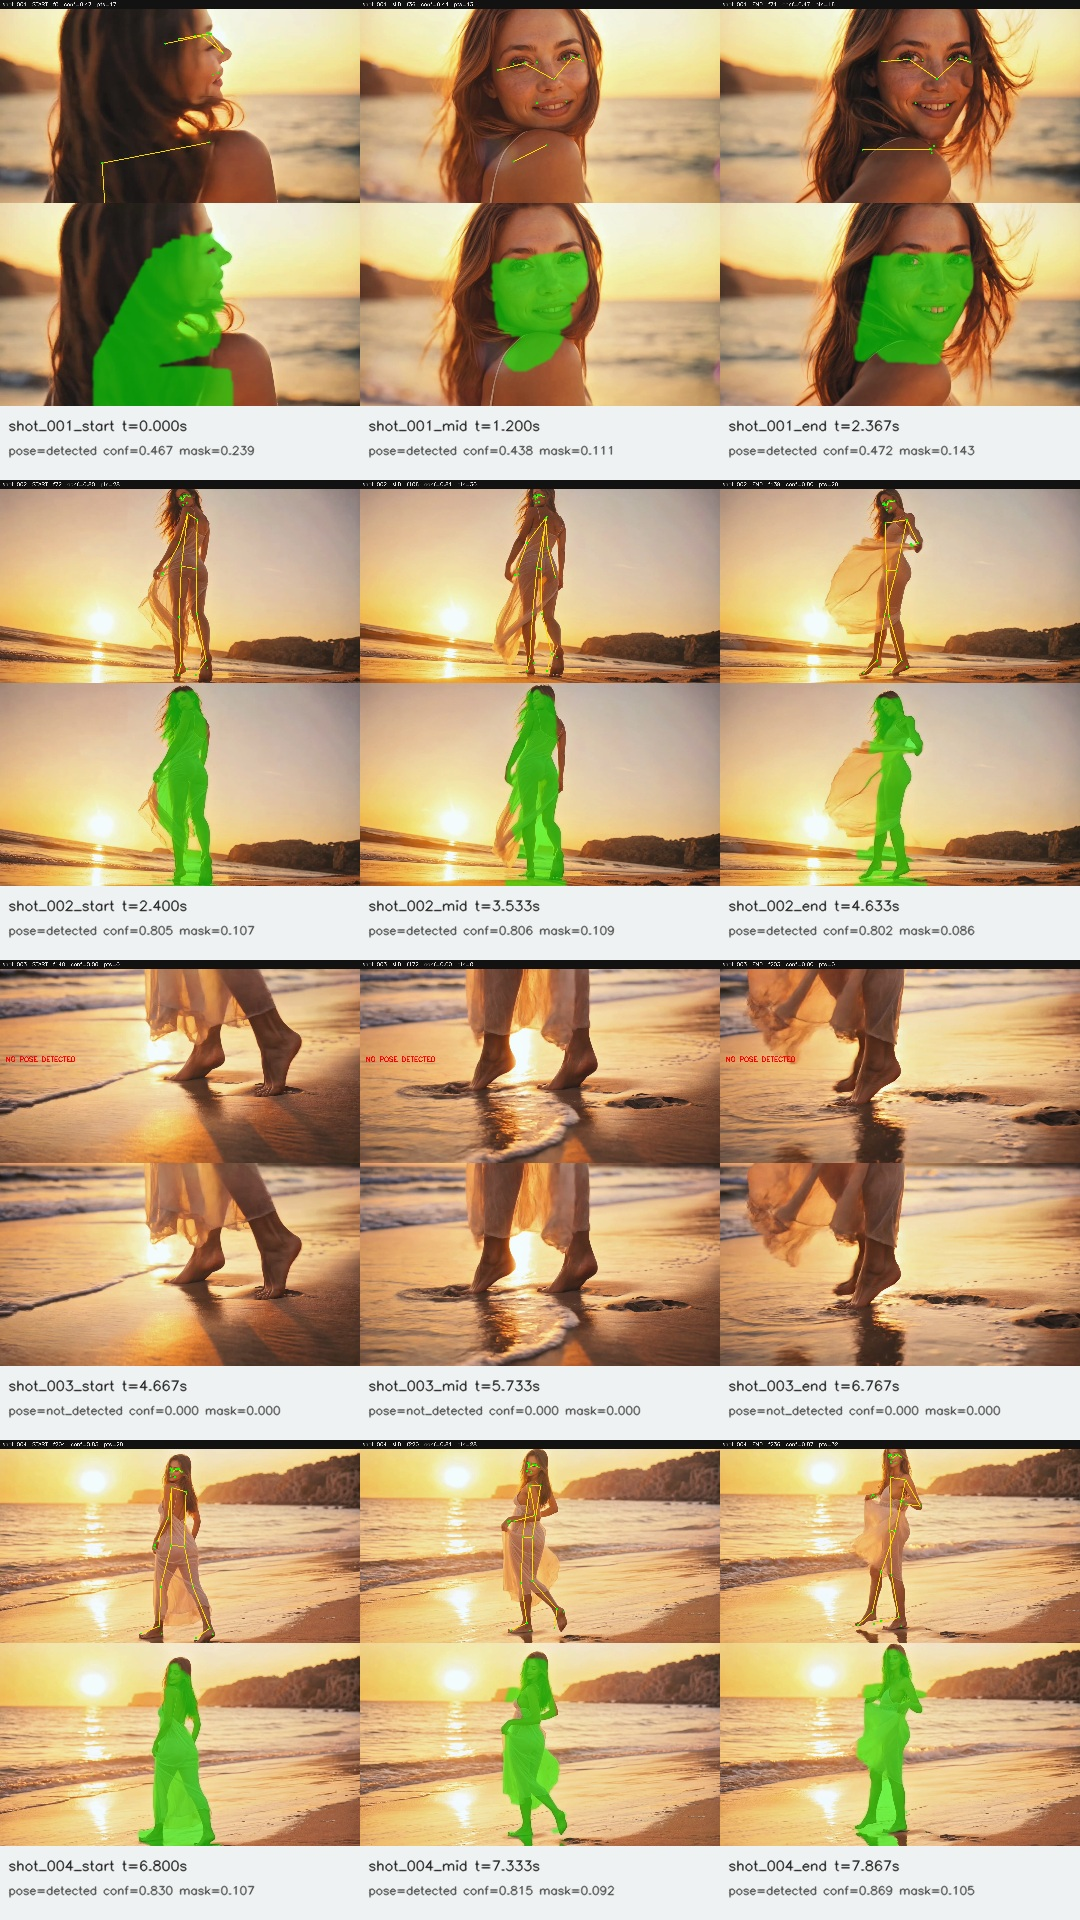
\includegraphics[width=0.62\textwidth,height=0.85\textheight,keepaspectratio]{figs/contact_sheet_reference_control_pose_mask_audit.jpg}
\par\vspace{3pt}{\footnotesize \textbf{Figure 4.2} --- Reference-control pose/mask audit contact sheet. The audit samples start/mid/end frames from each of the four beach-reference shots. Pose detections and pose-seeded GrabCut mask candidates are shown where available. Shot\_003, a feet-detail shot, produced no reliable pose seed and was marked unavailable. These outputs are included as control-signal reliability evidence, not as final generation inputs.}
\end{figure*}

\addcontentsline{toc}{subsection}{4.12 Complementary street-scene runs: scene-package replacement and archived pose-guidance branch}

\section*{4.12 Complementary street-scene runs: scene-package replacement and archived pose-guidance branch}

\begin{quotebox}
\textbf{Type:} executed (scene-package run, keyframe$\rightarrow$I2V$\rightarrow$assembly) + tested-and-archived (reference-structure pose branch). \quad \textbf{Input:} static street scene package, Look 3 identity anchors, \texttt{reference\_video = None}. \quad \textbf{Output:} \texttt{final\_look3\_street\_demo.mp4} (4 clips, human-reviewed); an archived start/end pose-guidance branch (\S{}3.5.5). \quad \textbf{Proves:} scene-package replacement with identity-anchor repair reaches a completed, human-approved final assembly. \quad \textbf{Does not prove:} reference-video-driven cross-scene recomposition (Mode A-2) --- this run used no reference video.
\end{quotebox}

\textbf{Framing.} The beach run (\S{}4.3--\S{}4.7) and the street runs are \textbf{complementary}, not primary versus secondary: the beach run proves the \emph{end-to-end closed loop} on a real reference video, while the street run (\texttt{live\_test\_04\_street\_look3}) is a \textbf{scene-package} run --- \texttt{reference\_video = None}, scene taken from a static street package --- that stresses identity consistency under scene replacement and is itself \textbf{completed end-to-end through keyframe $\rightarrow$ Kling I2V $\rightarrow$ final assembly} (\texttt{final\_look3\_street\_demo.mp4}; four clips, with prompt-only motion repair on shots 001 and 003, \S{}4.13). The street work has two parts: the completed \emph{scene-package run}, and a separate \emph{reference-structure} attempt (start/end pose transfer from the beach reference) that was tested and archived.

\textbf{Scene-package stage --- initial street run (\texttt{generate\_street\_run.py}).} The first street run used a manually specified four-shot plan (mirroring the beach shot types) with static Parisian-street references and Look 3 anchors, as an identity-consistency stress test in a new scene.

\textbf{Observed failure --- identity drift.} The model preserved the Parisian street environment and the Look 3 outfit, but the generated face drifted away from the intended character --- often re-interpreted as a generic brunette. This reflects a common limitation of multi-reference conditional generation: with identity, outfit, scene and framing references supplied simultaneously, the model tends to prioritise scene composition and garment appearance while averaging the facial identity.

\textbf{Repair --- front/profile identity anchors + reference-role separation.} An identity-anchor stage was introduced before per-shot keyframe generation, replacing the full look sheet (whose multiple poses and layout text dilute the facial signal) with two targeted anchors --- \textbf{front-facing} and \textbf{profile}. Reference ordering was then made shot-type dependent: for face-visible shots the identity anchor takes the strongest slot; for lower-body shots (e.g. the feet insert) the scene and outfit references remain dominant since no face is visible. \texttt{input\_fidelity="high"} was used for identity-critical shots, with a human review gate before any I2V step. The repair combines three levers: reference-role separation, shot-type-specific ordering, and high input fidelity.

As shown in Figure 4.3, the earlier outputs preserved the outfit and street scene but showed weaker facial fidelity; after the identity-anchor change the keyframes became more consistent with the intended character in both frontal and side-profile views. Consistent with the reporting rule of this chapter, this is a \textbf{qualitative, human-review} result: it \textbf{improves} identity consistency and \textbf{reduces} drift; it does not "solve" identity, and no ArcFace score is attached (automated scoring remains pending, \S{}4.10). Stronger identity methods --- IP-Adapter FaceID, InstantID, or a locally fine-tuned LoRA --- are considered \textbf{future work} rather than part of the current API-based implementation. The value of the result is methodological: identity consistency in multi-reference generation is not only a prompt-writing problem but depends on explicit reference-role separation and shot-type-specific reference ordering --- the same failure$\rightarrow$diagnosis$\rightarrow$targeted-repair pattern that defines the system's agentic loop.

\begin{figure*}[!tp]
\centering
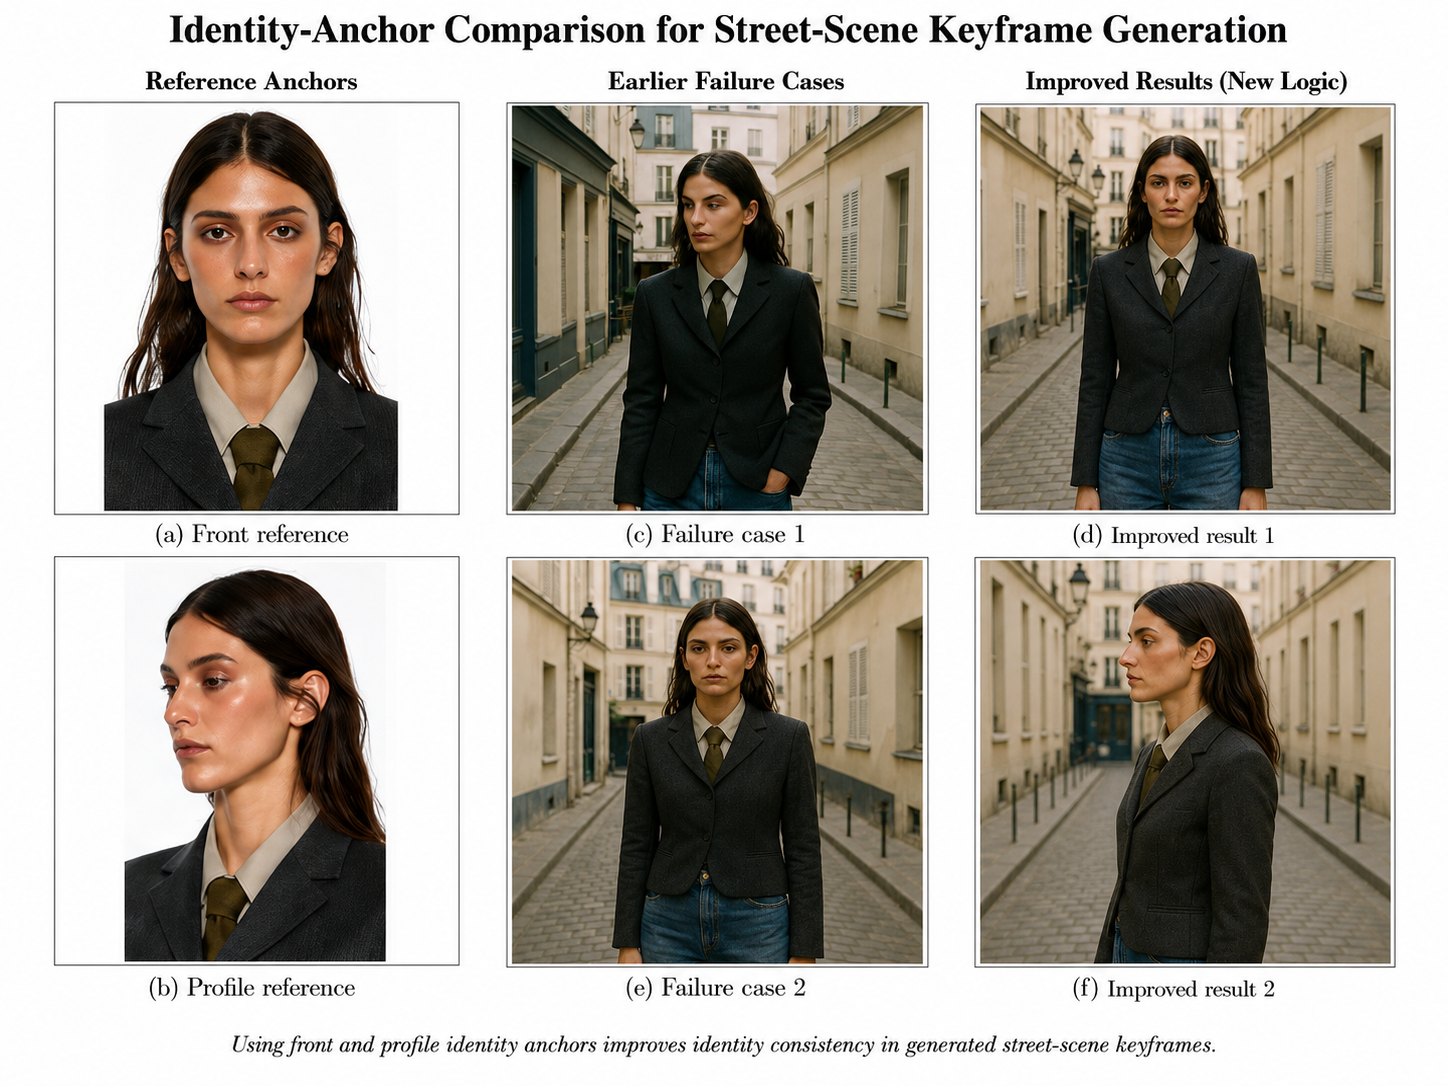
\includegraphics[width=\textwidth,height=0.85\textheight,keepaspectratio]{figs/street_identity_anchor_comparison.png}
\par\vspace{3pt}{\footnotesize \textbf{Figure 4.3} --- Identity-anchor comparison for street-scene keyframe generation (\textbf{qualitative human-review comparison; no automated ArcFace scoring}). Left: the front and profile identity references that define the character's facial structure. Middle: earlier failure cases that preserve the street environment and outfit but drift in facial identity. Right: improved results after the reference-ordering policy was revised to prioritise the identity anchor for face-visible shots. Identity consistency \textbf{improves qualitatively} --- particularly in the frontal and side-profile keyframes --- but is \textbf{not solved}; automated identity scoring remains pending (\S{}4.10).}
\end{figure*}

\textbf{Reference-structure stage --- tested and archived (\texttt{generate\_street\_start\_end.py}).} The street run was then extended into the concrete attempt at \emph{reference-structure reuse under scene replacement}: reading the beach reference's \textbf{start/mid/end pose metadata} (\S{}4.11) and applying the graded structural guidance of \S{}3.5.5 --- a rendered skeleton slot for the pose-reliable shots (shot\_002, shot\_004), head-orientation cues for shot\_001, framing/text only for shot\_003 (no pose). This branch was \textbf{implemented, run, inspected, and then archived} --- it is \textbf{not} part of the final output (\texttt{keyframes/start\_end/\_ARCHIVED\_experimental\_limitation.md}).

\textbf{Why it was rejected (a negative result).} The generated start/end keyframes did not reliably preserve the intended motion structure: START and END frames are generated independently, so a pair is not temporally coherent and is unusable as a Kling image/image-tail pair; shot\_001's head-orientation progression inverted; the shot\_002 skeleton specified a walk but the output rendered a frontal standing figure; shot\_003 never completed. The root cause is the \S{}3.5.5 boundary --- a skeleton image is too weak a control signal for \texttt{gpt-image-1}. This is a documented \textbf{experimental limitation}, not a core failure; reliable pose control remains future work, likely requiring a pose-conditioned backend.

\textbf{Final street output --- completed scene-replacement I2V.} The delivered result uses the approved \textbf{single-keyframe} run, not the start/end branch: four approved keyframes were animated with Kling v1.6 (std, 5 s) into four clips and assembled into \texttt{final\_look3\_street\_demo.mp4}. Identity, scene and look pass human visual review; automated ArcFace/DWPose scoring remains pending (\S{}4.10), and motion quality is audited quantitatively in \S{}4.13.

\emph{Summary.} Beach and street are complementary and both completed through I2V: beach demonstrates the end-to-end closed loop from a real reference video; street demonstrates scene replacement under an identity-drift $\rightarrow$ diagnosis $\rightarrow$ anchor repair $\rightarrow$ archived pose-extension arc. Reference-structure reuse is \emph{feasible} for per-shot planning but \emph{not reliable at generation} with the current backend.

\addcontentsline{toc}{subsection}{4.13 Motion-energy audit of the generated clips}

\section*{4.13 Motion-energy audit of the generated clips}

\textbf{Type: Executed (local optical-flow analysis; no API, no Kling).} Successful clip generation (\S{}4.5) does not by itself guarantee natural motion, and the three-frame clip-review sheets are too sparse to judge it. A dense \textbf{motion-energy audit} was therefore run locally on the street run: each reference shot segment and each generated clip is decoded, resized to a common height (288 px, native aspect preserved --- reference 16:9, clips 2:3, no squeezing), and per consecutive frame pair a Farneb\"ack (Farneb\"ack, 2003) optical-flow magnitude is computed, reported as \textbf{\% of frame height per frame}. The reference video is the \textbf{motion target} (the author-created reference clip); the beach generated clip is a \textbf{secondary generated-output baseline}, not a target. "Captured \%" is generated flow $\div$ reference flow for the same shot, computed per-frame so the 5 s clip vs \textasciitilde{}2 s reference segment does not bias it.

\begin{table*}[t]
\centering
{\footnotesize\textbf{\textbf{Table 4.15 --- Motion-energy audit: mean optical flow (\% frame-height/frame) and capture rate (Executed)}}}\par\vspace{3pt}
\scriptsize
\begin{tabularx}{\textwidth}{l>{\RaggedRight\arraybackslash}Xll>{\RaggedRight\arraybackslash}Xl>{\RaggedRight\arraybackslash}X}
\toprule
shot & Reference avg / peak & Street & Street captured & Beach (baseline) & Beach captured & Reference motion character \\
\midrule
shot\_001 & 0.336 / 1.48 & 0.047 & \textbf{14\%} & 0.084 & 25\% & energetic head-turn to camera \\
shot\_002 & 0.119 / 0.49 & 0.044 & \textbf{37\%} & 0.077 & 65\% & calm slow walk away (lowest-motion ref) \\
shot\_003 & 0.753 / 2.57 & 0.141 & \textbf{19\%} & 0.189 & 25\% & most active: stepping feet + turn \\
shot\_004 & 0.273 / 0.83 & 0.175 & \textbf{64\%} & 0.186 & 68\% & lateral walk with camera movement \\
\bottomrule
\end{tabularx}
\end{table*}

\emph{Findings.} The street clips reproduce only \textbf{14--64\%} of the reference's per-frame motion energy, and both generations under-animate on every shot (neither street nor beach exceeds 68\% of the reference). The two largest deficits are exactly the reference's two most energetic moments --- shot\_001 (quick head-turn, 14\% captured) and shot\_003 (active feet-step + turn, 19\%): single-still I2V \textbf{flattens motion peaks}. The calm reference shot (shot\_002) is reproduced proportionally better because the reference itself is low-motion there. The street-vs-beach gap is small; the dominant gap is generation-vs-reference. This converts the earlier subjective "the clips feel under-animated" into a quantified, reproducible measurement.

\emph{Honest boundary.} This is a motion-\textbf{energy / amplitude} comparison, \textbf{not} a claim of frame-level motion transfer: the reference clip shows a different outfit and framing, so only per-frame motion magnitude and speed are compared, never pixel correspondence. The dense filmstrips are qualitative motion views, \textbf{not} frame-aligned evidence --- the generated clips are not temporally synchronised with the reference shots.

\emph{Diagnosis.} The audit attributes part of the motion loss to \textbf{damping language leaking from the Look package} --- Look 3 attitude words ("quiet", "composed", "unhurried") and prompt hedges ("slow", "subtle", "minimal") suppress motion.

\emph{Prompt-level motion repair --- executed and verified.} Acting on that diagnosis, a \textbf{prompt-only} repair was applied to the two lowest-energy shots (shot\_001, shot\_003) \textbf{without regenerating any keyframe}: the Look block was restricted to identity/outfit, and a separate \textbf{Motion block} was written from observable reference cues (head-turn speed, stride visibility, body displacement, footstep rhythm); Kling was then re-run for those two shots only (\texttt{shot\_001\_look3\_street\_motion\_v2.mp4}, \texttt{shot\_003\_look3\_street\_motion\_v2.mp4}) and promoted into a motion-v2 preview assembly. Re-running the optical-flow audit on the new clips confirms a substantial improvement (Table 4.16): shot\_001 rises from \textbf{14\% to 51\%} of the reference motion energy and shot\_003 from \textbf{19\% to 47\%}, with identity and scene unchanged (keyframes untouched). (Values as recorded in the run's \texttt{decision\_log.json} \texttt{recovered\_motion\_pct} fields.)

\begin{table*}[t]
\centering
{\footnotesize\textbf{\textbf{Table 4.16 --- Prompt-level motion repair: captured \% of reference before/after (Executed)}}}\par\vspace{3pt}
\footnotesize
\begin{tabularx}{\textwidth}{lll>{\RaggedRight\arraybackslash}X}
\toprule
shot & before (v1) & after (v2) & keyframe regenerated? \\
\midrule
shot\_001 & 14\% & \textbf{51\%} & no \\
shot\_003 & 19\% & \textbf{47\%} & no \\
\bottomrule
\end{tabularx}
\end{table*}

This closes a second, \textbf{motion-level} agentic repair loop --- \emph{generate $\rightarrow$ audit $\rightarrow$ diagnose $\rightarrow$ prompt-only fix $\rightarrow$ selective re-run $\rightarrow$ re-audit $\rightarrow$ promote} --- distinct from the keyframe identity loop, and it isolates the fix to language (appearance separated from motion), not to new keyframes. It does \textbf{not} reach parity --- single-still I2V cannot reproduce 100\% of the reference clip's motion energy --- so a residual gap remains, but the targeted shots roughly tripled their captured motion. (The before/after values were independently recomputed here with the same Farneb\"ack optical-flow method, which reproduces the original 14\%/19\% exactly.)

\begin{figure*}[!tp]
\centering
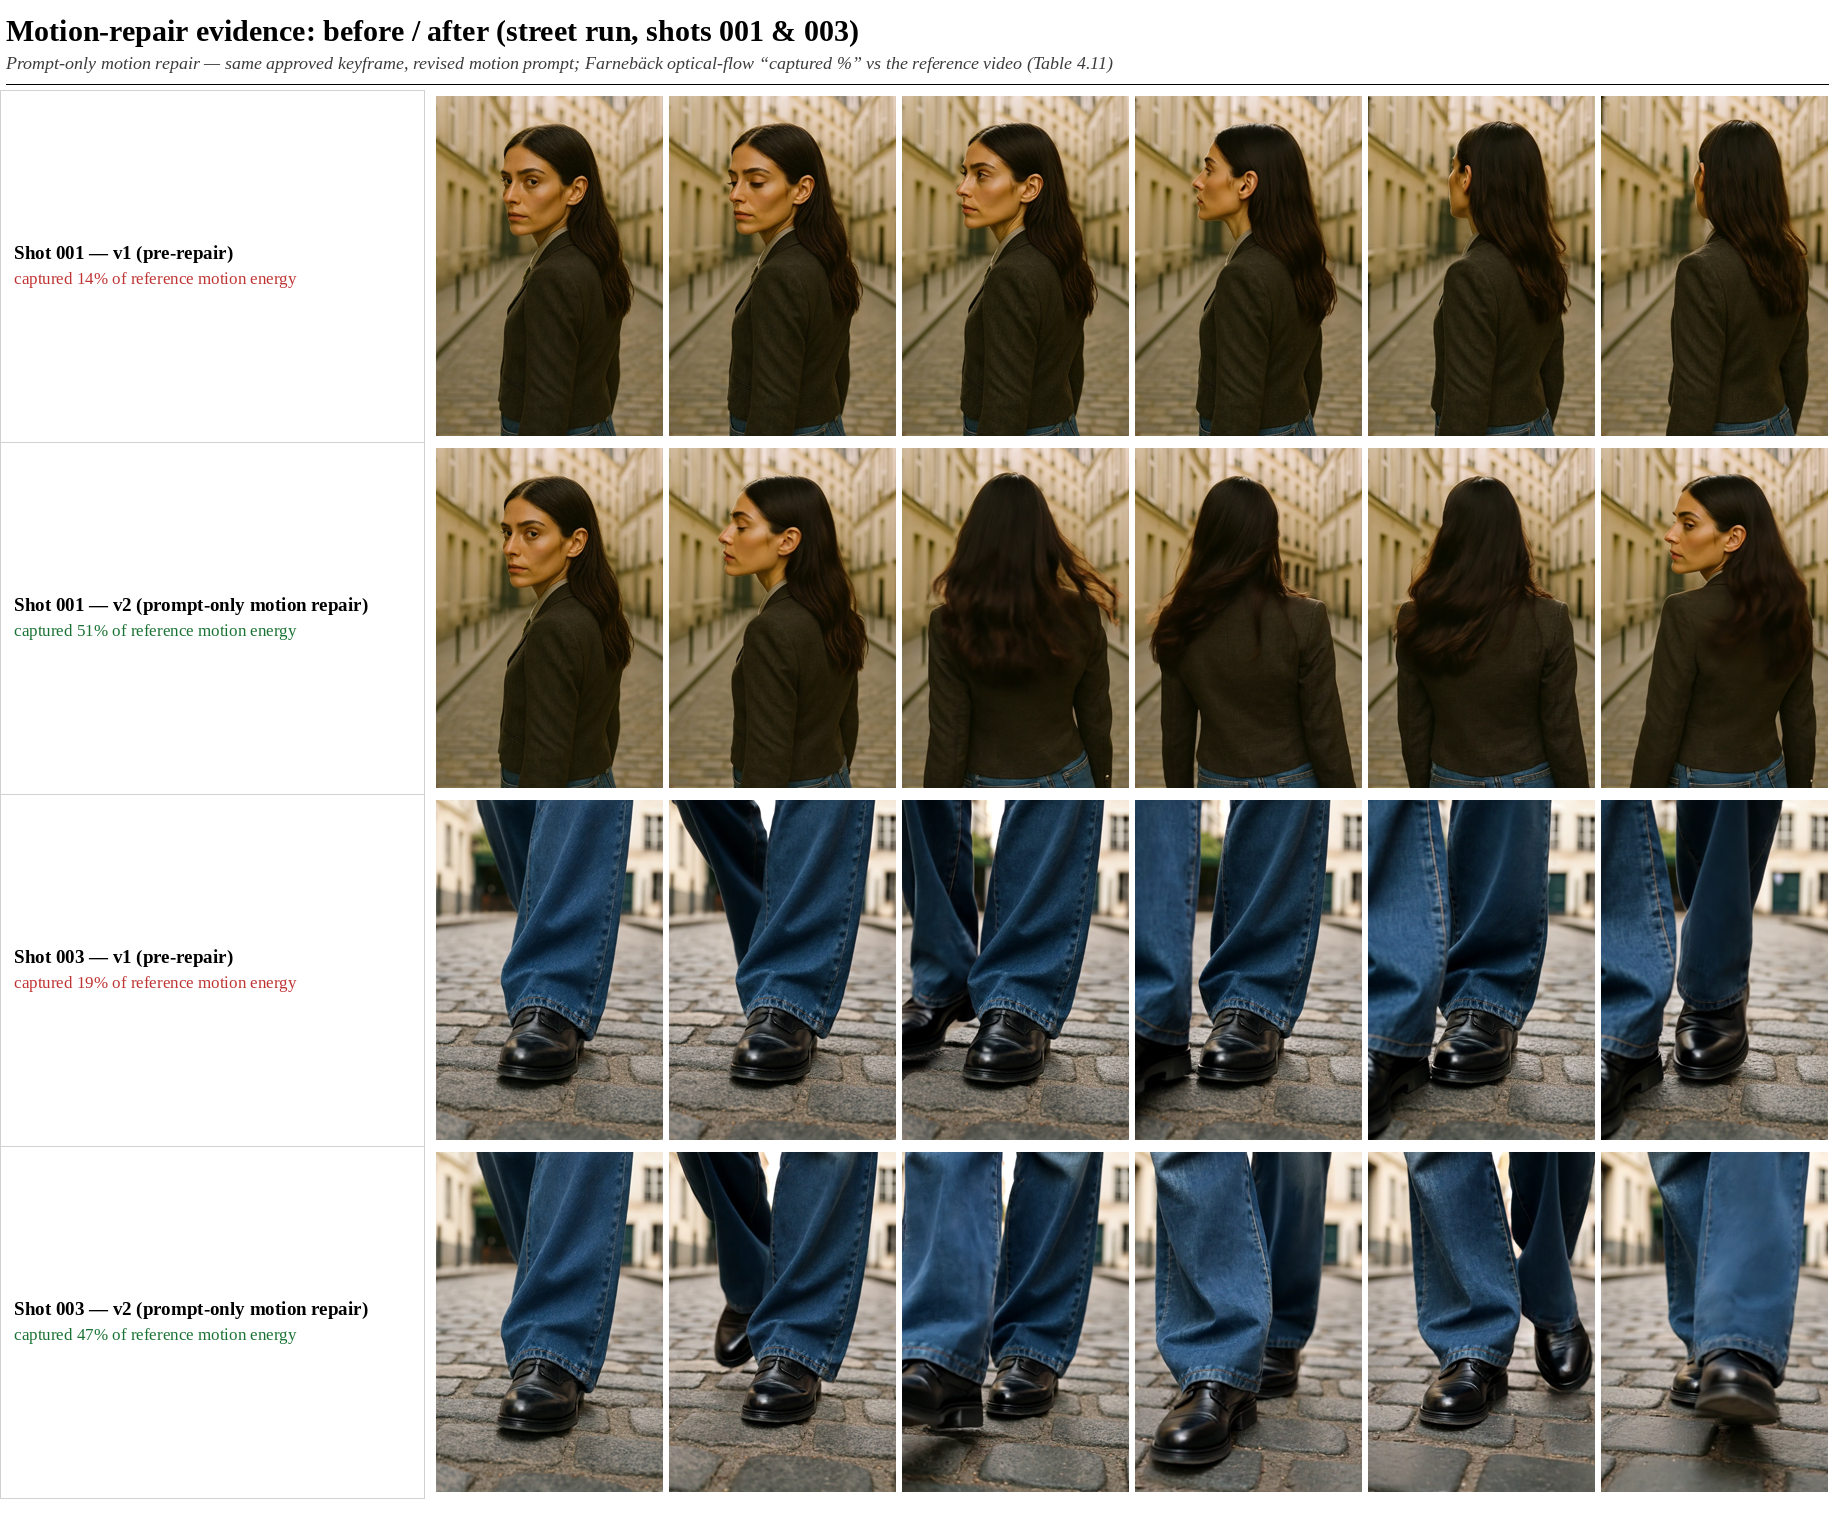
\includegraphics[width=\textwidth,height=0.85\textheight,keepaspectratio]{figs/motion_repair_before_after.png}
\par\vspace{3pt}{\footnotesize \textbf{Figure 4.4} --- Motion-repair evidence, sampled frames from the actual v1/v2 clips underlying Table 4.16. Top two rows: shot\_001 before (14\% captured) and after (51\%) the prompt-only motion repair --- the head-turn amplitude visibly increases from a slight glance to a full turn toward camera. Bottom two rows: shot\_003 before (19\%) and after (47\%) --- stride and body displacement become clearly visible. Identity, outfit and the approved keyframe are unchanged between v1 and v2; only the Motion prompt block was rewritten (\S{}4.13).}
\end{figure*}

\addcontentsline{toc}{subsection}{4.14 Experimental development process and negative results}

\section*{4.14 Experimental development process and negative results}

The system was not correct on the first attempt; it was developed as an iterative \textbf{failure $\rightarrow$ diagnosis $\rightarrow$ repair $\rightarrow$ result} chain. This section consolidates that trajectory, because the intermediate failures --- reported here as \textbf{negative results} --- are themselves the evidence for why an explicit orchestration layer is needed rather than a direct API call.

\textbf{Motivation (development observation).} During development, the hosted ChatGPT image-generation workflow produced more immediately usable multi-reference keyframes than direct calls to the \texttt{gpt-image-1} Images API. This should \textbf{not} be interpreted as evidence that the underlying image model is intrinsically superior; rather, it suggests that the hosted interface may apply additional, undisclosed orchestration --- prompt expansion, conversational state retention, reference-role interpretation, candidate selection, or iterative self-correction. The API exposes the generation primitive directly, so these control mechanisms had to be reconstructed \textbf{explicitly} inside the pipeline (\S{}3.1.1). This is a \textbf{qualitative development observation}, not a controlled experiment; a matched comparison (identical references, prompts and attempt budget) is proposed as future work (Table 4.17).

The development proceeded in four stages, each a documented failure and its repair:

\begin{enumerate}[leftmargin=1.4em,itemsep=2pt,topsep=2pt]

\item \textbf{Multi-reference competition.} With identity, outfit, scene and framing references supplied at once, scene and outfit were preserved but facial identity was \textbf{averaged} into a generic brunette. \emph{Diagnosis:} the references compete for control and the model trades identity for scene/garment fidelity (\S{}4.12, scene-package stage).

\item \textbf{Reference-slot reordering.} A single fixed reference order does not suit every shot: face-visible shots need the identity anchor prioritised, while feet/lower-body shots need the scene/source frame prioritised. \emph{Repair:} shot-type-specific slot ordering plus reference-role separation (\S{}3.5.1, \S{}4.12), which reduced identity drift (Figure 4.3).

\item \textbf{Skeleton-guidance experiment (archived negative result).} Start/middle/end poses were extracted and neutral skeletons rendered (\S{}4.11), but \texttt{gpt-image-1} follows a skeleton \emph{image} only weakly; the start/end keyframes were incoherent and did not adopt the intended pose. \emph{Outcome:} the branch was tested and \textbf{archived}, excluded from the final output (\S{}3.5.5, \S{}4.12).

\item \textbf{Motion-intensity repair.} The first Kling clips were under-animated; optical-flow analysis showed only \textbf{14--64\%} of the reference motion energy (\S{}4.13, Table 4.15). \emph{Repair:} a prompt-only motion fix (appearance separated from motion) re-ran shot\_001 and shot\_003 and raised them to \textbf{51\%} and \textbf{47\%} without regenerating keyframes (Table 4.16).

\end{enumerate}

A further \textbf{documented control-signal trial} supports the same design decision from the analysis side: the reference-control pose/mask audit (\S{}4.11.1) quantified per-shot control-signal reliability (9/12 samples usable; the feet-detail shot unavailable; close-up framing weaker) and confirmed that pose and mask extraction serve as diagnostic and candidate-control evidence rather than production-ready hard controls --- reinforcing the choice of the keyframe-first, prompt-level, human-gated path for the final evidence.

Read together, these stages are the project's contribution narrative: \emph{ChatGPT-style output motivated the design $\rightarrow$ the raw API initially failed $\rightarrow$ the failures were diagnosed $\rightarrow$ explicit reference-role separation, slot ordering, a decision log and targeted repair were added $\rightarrow$ the result is the current agentic workflow.} The negative results (the skeleton branch; the residual motion gap) are not signs of an unfinished project but the evidence that the orchestration layer is necessary --- and, unlike a hosted interface, its behaviour here is recorded, evaluable and reproducible.

\begin{table*}[t]
\centering
{\footnotesize\textbf{\textbf{Table 4.17 --- Proposed controlled comparison: hosted workflow vs. direct-API pipeline (Planned; future work, not yet run)}}}\par\vspace{3pt}
\footnotesize
\begin{tabularx}{\textwidth}{>{\RaggedRight\arraybackslash}Xl>{\RaggedRight\arraybackslash}X}
\toprule
Metric & Hosted workflow & Direct-API pipeline \\
\midrule
First-attempt approval rate & \emph{pending} & \emph{pending} \\
Identity consistency (ArcFace) & \emph{pending} & \emph{pending} \\
Framing adherence & \emph{pending} & \emph{pending} \\
Outfit fidelity & \emph{pending} & \emph{pending} \\
Manual prompt revisions & \emph{pending} & \emph{pending} \\
Average attempts per shot & \emph{pending} & \emph{pending} \\
Latency and cost & \emph{pending} & \emph{pending} \\
\bottomrule
\end{tabularx}
\end{table*}

A matched protocol (identical reference images and prompts, an equal attempt budget, and the same reviewer) would be required to turn this development observation into a formal result; no such comparison is claimed here.

\addcontentsline{toc}{subsection}{4.15 Limitations and threats to validity}

\section*{4.15 Limitations and threats to validity}

The limitations fall into three groups --- limits of the \textbf{system}, limits of the \textbf{experimental design}, and boundaries on \textbf{what this chapter argues}. Reporting them in full is part of the chapter's honesty rule; several are the direct counterpart of the positive results above.

\addcontentsline{toc}{subsubsection}{4.15.1 System limitations}

\subsection*{4.15.1 System limitations}

\begin{enumerate}[leftmargin=1.4em,itemsep=2pt,topsep=2pt]

\item \textbf{The agentic loop is partially automated (human-gated).} On the reported runs the loop that operated was \emph{human review $\rightarrow$ diagnose $\rightarrow$ modify prompt / reference order $\rightarrow$ regenerate} (the logged decision loop), not the fully automatic \emph{scoring $\rightarrow$ diagnosis $\rightarrow$ targeted repair $\rightarrow$ re-evaluation}. The system is best described as \textbf{a partially automated agentic workflow with a human-gated repair loop}; the stronger claim of a fully automated evaluation--repair loop awaits the automated scoring and the loop-ON-vs-OFF ablation (\S{}4.8--\S{}4.10).

\item \textbf{Structure-guided regeneration, not motion transfer.} The system extracts shot boundaries, framing, a broad camera-motion class, action intent, start/mid/end pose and beat timing, but does \textbf{not} reproduce exact step cadence, per-frame limb trajectories, stride length, body-speed curves or the reference camera path. It should be described as \emph{reference-structure-guided regeneration} --- never \emph{motion transfer}, \emph{reenactment} or \emph{exact replication}. In short: the system preserves reference shot structure and action intent, but does not perform exact frame-level motion transfer.

\item \textbf{Single-keyframe I2V under-conditions the temporal sequence.} Each shot is animated from one approved keyframe, so the start composition is controlled but the end is not: face, garment detail and camera end-point can drift across the clip. Start/end or multi-keyframe conditioning and pose-sequence constraints are future work --- the start/mid/end pose is currently used for \emph{analysis}, not as generation constraints.

\item \textbf{Reference structure is not reliably transmitted to I2V.} Kling receives an approved keyframe and a natural-language motion prompt, not the reference optical flow or a per-frame pose sequence. Even when a keyframe's pose is close to the reference, the animation can change gait, orientation, amplitude or timing, or introduce camera motion --- which is why shot\_001 and shot\_003 lost the most motion energy (\S{}4.13).

\item \textbf{Multi-reference competition and the identity--pose--scene--look trade-off.} Supplied together, identity, look, scene and source-frame references compete for the model's attention. Fixed slot ordering is a \textbf{tested heuristic}, not a hard constraint the model guarantees, and it can vary with shot type, model version and prompt. Because the factors are not truly decoupled inside the model, a \emph{targeted repair} can cause collateral changes (strengthening identity may alter framing; strengthening scene may shift lighting/skin tone), so \textbf{all} metrics --- not only the repaired one --- must be re-checked after a repair. Repair is therefore \textbf{diagnosis-guided and probabilistic}, not a guaranteed correction.

\item \textbf{Metrics are operational proxies, not cinematic quality.} Even once ArcFace / DWPose / framing / beat are computed, they measure selected consistency dimensions, not overall quality: temporal flicker, anatomy errors, garment consistency, facial naturalness, motion smoothness, aesthetics and inter-shot continuity are uncovered. Identity in particular should not rest on a single embedding metric (ArcFace is unstable on profile, occluded, small, blurred, back-view or feet-only shots, which should score \texttt{not\_applicable} rather than a wrong low value). \emph{The metrics act as operational proxies for selected consistency dimensions, not a complete measure of cinematic quality.}

\item \textbf{Format, timing, cost and external dependencies.} Fixed \textasciitilde{}5 s Kling clips make the output (\textasciitilde{}20.4 s) longer than the reference (\textasciitilde{}7.9 s) and do not preserve per-shot durations; the delivered format is 2:3 (768$\times$1152), not strict 9:16 (\texttt{gpt-image-1}'s 1024$\times$1536 limit). The pipeline is high-latency, not real-time, and depends on closed external services (OpenAI images / GPT-4o Vision / Kling) plus MediaPipe, PySceneDetect and librosa: the \emph{architecture} is reproducible but \emph{pixel-level output} is bound to specific model versions and the execution date. Copyright handling is \textbf{risk reduction, not a guarantee} (shot-sequence originality, character-usage rights and opaque third-party training data remain open).

\end{enumerate}

\addcontentsline{toc}{subsubsection}{4.15.2 Experimental-design limitations}

\subsection*{4.15.2 Experimental-design limitations}

\begin{enumerate}[leftmargin=1.4em,itemsep=2pt,topsep=2pt]

\item \textbf{Small single case.} One reference video, four shots, one character/look and two environments support a \textbf{proof of concept}, not a claim of general improvement; multi-character, dialogue, fast action, occlusion, indoor lighting, long-form and stylised content are unvalidated. Multi- character interaction in particular (identity assignment, gaze, contact, occlusion) is untested.

\item \textbf{No equal-budget baseline.} The chapter lacks matched baselines --- prompt-only, unstructured multi-reference, fixed-slot-without-repair, full-pipeline-with-repair, and the hosted workflow as a qualitative point. Without an \textbf{equal-compute} comparison (attempts, API calls, cost, time) the gain cannot be attributed cleanly to targeted repair rather than to extra sampling; the decisive test --- \emph{targeted repair $\times$ N attempts vs. blind reroll $\times$ N attempts} --- is future work.

\item \textbf{Author-conducted review and selective-reporting risk.} Identity and quality judgements were made by the author, who also designed the system and selected the outputs, so confirmation bias is possible: the human review here is \textbf{author-conducted visual inspection}, not a blind study with independent raters and a predefined rubric. To limit selective reporting, total generations, accepted/rejected counts and unrecovered failures are reported in full from the decision log.

\end{enumerate}

\addcontentsline{toc}{subsubsection}{4.15.3 Argument and scope boundaries}

\subsection*{4.15.3 Argument and scope boundaries}

\begin{enumerate}[leftmargin=1.4em,itemsep=2pt,topsep=2pt]

\item \textbf{The ChatGPT observation is a workflow observation, not a model comparison.} The hosted interface may apply undisclosed prompt rewriting, routing, candidate ranking or version selection, so the correct statement is: \emph{under the tested interaction conditions, the hosted workflow required less explicit orchestration to obtain usable multi-reference keyframes} --- not that its image model is superior. Because the hosted backend changes over time, this observation has limited reproducibility.

\item \textbf{Analysis tools are heuristic and content-specific.} The camera-motion label is a heuristic estimate (it can confuse push-in with subject approach, pan with parallax, handheld with subject motion), not camera-parameter recovery; shot detection and beat alignment suit \textbf{rhythmically edited short-form video with visually distinguishable shots}, not dissolves, long takes or non-beat-driven material.

\end{enumerate}

\textbf{Scope statement.} \emph{The current system should therefore be understood as a proof-of-concept for auditable, reference-structured and selectively repairable short-form video generation, rather than a general-purpose system for exact motion transfer or fully autonomous cinematic production.}

\addcontentsline{toc}{subsection}{4.16 Summary}

\section*{4.16 Summary}

On \texttt{live\_test\_03\_4shots} the pipeline is demonstrated \textbf{end to end}: a 7.92 s / 123 bpm four-shot reference was decomposed into four complete five-track storyboard units (Table 4.3), four keyframes were generated and human-approved through a logged diagnose-and-retry process (Table 4.5), four Kling I2V clips were produced (Table 4.6), and the clips were assembled into a single \texttt{ffprobe}-confirmed 768$\times$1152, 20.4 s vertical short (Table 4.7). The \textbf{verified result is a successful end-to-end generation under human visual review}, with real evidence of self-correcting generation from the decision log. The \textbf{automated metric layer} (identity, pose, framing, beat) and the \textbf{baseline-vs-agentic ablation} are designed and staged (Tables 4.6--4.7) but were \textbf{not run in-loop} on this batch. Only the ArcFace identity diagnostic has been computed post-hoc (\S{}4.8.1); the full in-loop automated metric layer was not executed. Computing the remaining metrics is the next evaluation step and the point at which the loop's contribution becomes quantitative, within the claim boundary stated in \S{}3.5.3.

The complementary \textbf{street run} (\texttt{live\_test\_04\_street\_look3}) is now also completed through I2V: after an iterative identity-anchor repair (\S{}4.12), four approved keyframes were animated into four clips and assembled into a final scene-replacement video. Two honest negative results accompany it: the start/end skeleton-guidance branch was tested and archived (skeleton reference too weak for \texttt{gpt-image-1}, \S{}4.12), and the motion-energy audit (\S{}4.13, Table 4.15) quantified that the initial street clips reproduce only 14--64\% of the reference's per-frame motion. Acting on the audit, a \textbf{prompt-only motion repair} (appearance separated from motion, no keyframe regeneration) then raised the two worst shots from 14$\rightarrow$51\% and 19$\rightarrow$47\% (Table 4.16) --- closing a second, motion-level agentic repair loop. These are reported as genuine engineering findings, not failures.

\addcontentsline{toc}{subsection}{4.17 Mode C --- driving-video backend: Condition A feasibility (Executed), Condition B (planned)}

\section*{4.17 Mode C --- driving-video backend: Condition A feasibility (Executed), Condition B (planned)}

\begin{quotebox}
\textbf{Type:} executed (Condition A, Phase 0 feasibility) + designed, not yet run (Condition B). \quad \textbf{Input:} driving performance video (\texttt{mode\_c.MP4}), DWPose skeleton + SAM-style mask (\S{}3.10), Wan2.2-Animate via Wan2GP on a remote RTX 4080. \quad \textbf{Output:} one 480$\times$848, \textasciitilde{}2.7 s replacement segment with motion followed and background preserved (Table 4.18). \quad \textbf{Proves:} the flagged pose-conditioned backend runs end to end on available hardware for a short segment. \quad \textbf{Does not prove:} production-scale (27 s) generation, exact identity fidelity, or integration into Mode A.
\end{quotebox}

This section reports a \textbf{future-work feasibility probe}, beyond the main Mode A evaluation above. Sections \S{}3.5.5 and \S{}4.15 flagged a pose-conditioned / driving-video backend as the route to reliable structural control; Mode C (\S{}3.10) tests whether such a backend is feasible on available hardware and how it behaves. Mode C has \textbf{two conditions} (\S{}3.10): \textbf{Condition A} (background-preserving replacement) was run as a Phase 0 probe and is reported below; \textbf{Condition B} (full replacement with scene regeneration) is designed but not yet run and is summarised at the end. Mode C uses a different backend and character and is not integrated into Mode A.

\textbf{Condition A --- Type: Executed (Phase 0; separate GPU backend; human review).} The local dashboard host has no GPU, so Mode C ran on a remote \textbf{RTX 4080 (16 GB, CUDA 12.9)}. The official Wan2.2-Animate 14B repository hit a flash-attn ABI mismatch on the installed torch build, so the working low-VRAM path was \textbf{Wan2GP} (int8 quantisation + mmgp CPU-offload, SDPA attention). One short, low-resolution single segment was generated end to end: \textbf{480$\times$848, 81 frames (\textasciitilde{}2.7 s at 30 fps)}, from a full-body driving window cut from the driving performance video (\texttt{mode\_c.MP4}).

\begin{table*}[t]
\centering
{\footnotesize\textbf{\textbf{Table 4.18 --- Mode C Condition A Phase 0 feasibility (Executed; human visual review)}}}\par\vspace{3pt}
\footnotesize
\begin{tabularx}{\textwidth}{>{\RaggedRight\arraybackslash}X>{\RaggedRight\arraybackslash}X}
\toprule
Aspect & Result \\
\midrule
Backend & Wan2.2-Animate via Wan2GP (int8 + mmgp CPU-offload, SDPA) \\
Hardware & RTX 4080, 16 GB, CUDA 12.9 \\
Segment & 480$\times$848, 81 frames (\textasciitilde{}2.7 s, 30 fps), single low-res segment \\
Runs on 16 GB VRAM & \ding{51} yes \\
Motion follows the driving video & \ding{51} yes (human review) \\
Background preserved outside the mask & \ding{51} yes (human review) \\
Body proportions / silhouette & come from the \textbf{driving video}, not the reference \\
Identity & similar, not exact (no LoRA / InstantID); distorts on extreme poses \\
Full 27 s generation & \ding{55} not validated (Phase 0 only) \\
Automated pose-similarity / identity scores & \emph{pending} (same rule as this chapter) \\
\bottomrule
\end{tabularx}
\end{table*}

\begin{figure*}[!tp]
\centering
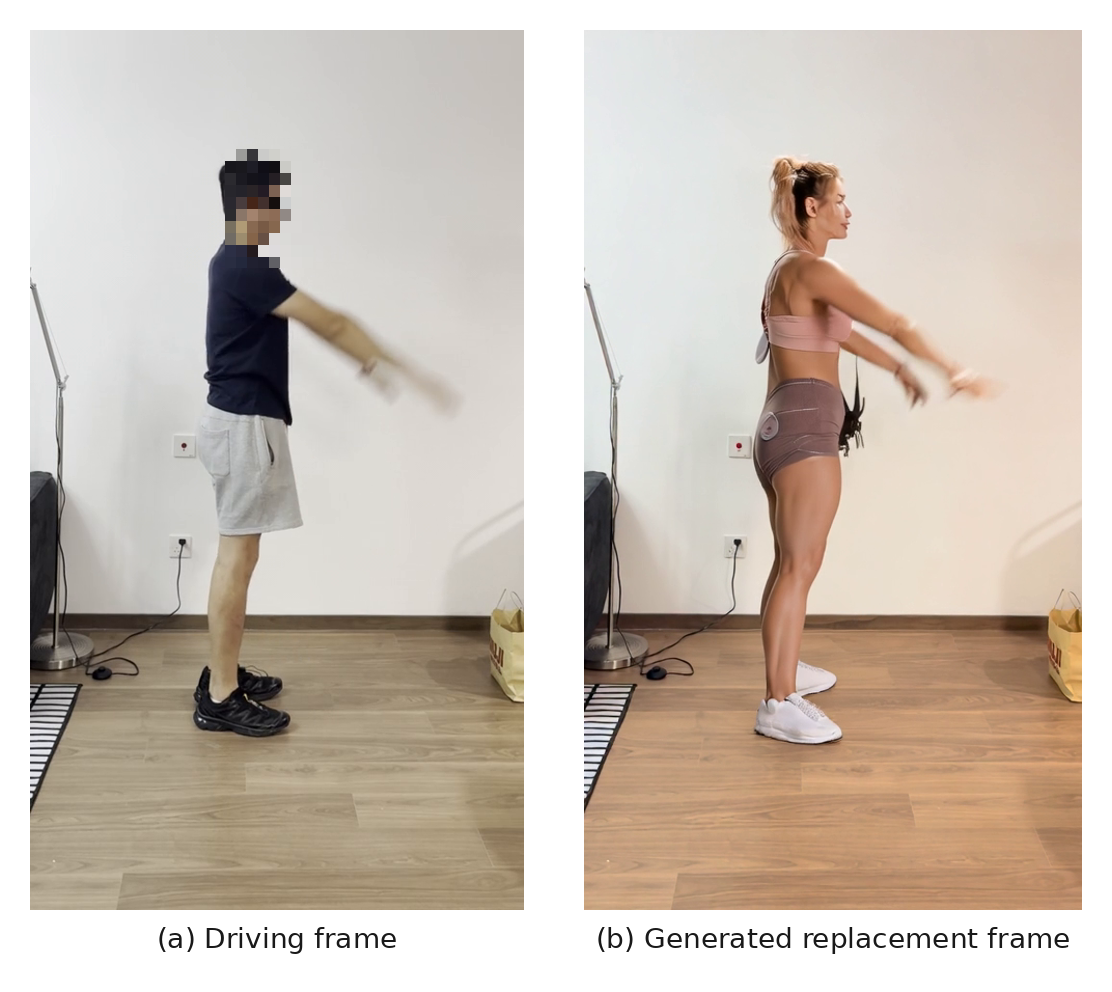
\includegraphics[width=\textwidth,height=0.85\textheight,keepaspectratio]{figs/mode_c_result.png}
\par\vspace{3pt}{\footnotesize \textbf{Figure 4.5} --- Mode C (Condition A) person replacement --- \textbf{Phase 0 low-resolution output (480$\times$848, \textasciitilde{}2.7 s); not final production quality}. A driving video frame (a) conditions Wan2.2-Animate replacement, producing the generated target-character frame (b) in the \textbf{workout-matched Look 1 (the 7 July target-look reference), distinct from Mode A's Look 3}: the character adopts the driver's pose and the room background is preserved, while proportions and silhouette follow the driver and identity is similar-not-exact (no identity fine-tuning). Per-frame preprocessing (DWPose skeleton + SAM-style person mask) is shown in Figure 3.10. The driving performer's face is anonymised (\S{}5.2).}
\end{figure*}

\textbf{Findings.} On 16 GB the segment ran end to end; the generated character \textbf{follows the driving motion} and the \textbf{background outside the mask is preserved} (Figure 4.5). Two limitations are clear and, importantly, they \emph{corroborate the rest of this chapter} rather than contradict it. First, \textbf{body proportions and silhouette are inherited from the driving performer, not from the reference} --- this is direct experimental confirmation of the reference-role boundary argued throughout (driving = motion / body / silhouette; reference = appearance / texture). Second, \textbf{identity is similar but not exact} and degrades on extreme poses, consistent with the identity-drift finding of \S{}4.12 and the absence of a LoRA / InstantID identity method. Quality is by human visual review; automated pose-similarity and identity scores are pending, and the full 27 s generation is not validated.

\emph{Positioning.} Mode C therefore does what \S{}3.5.5 and \S{}4.15 said was needed: it shows the pose-conditioned driving-video backend is \textbf{feasible on available hardware} and that pose is followed as a genuine per-frame control (unlike the weak skeleton-image guidance of \S{}3.5.5). It is reported as a feasibility extension --- not a completed, integrated third mode --- and it strengthens, by independent means, the reference-role and identity conclusions of the main evaluation.

\textbf{Extension run (executed 4 August 2026).} The Condition A backend was subsequently exercised on the full 7\,s driving clip (\texttt{test2.mov}, 209 frames at 30 fps) via the Wan2GP low-VRAM path (Wan2.2-Animate 14B, int8, replacement mode with automatic relighting LoRA), completing three end-to-end generations at 544$\times$960 across three 81-frame sliding windows ($\approx$2\,h\,55\,m per run on the 16\,GB RTX 4080). Motion following and background preservation held under human review; identity and proportion distortion on extreme poses persists (quality WIP), and window-boundary continuity is a new observed artefact. The full 27.15\,s driving video remains \textbf{not validated}. The session ended with a GPU driver fault on the remote host, recorded as an operational risk of long 14B runs on 16\,GB.

\textbf{Condition B --- full replacement / animation (planned).} Condition B regenerates the scene rather than preserving it, so its evaluation differs from Condition A: \textbf{background preservation} (a masked-pixel difference outside the person) does not apply; instead the metrics are \textbf{scene coherence}, plus the same \textbf{motion-follow} and \textbf{identity} checks. No Condition B output exists on disk at the time of writing, so it is reported here as the backend's planned second condition --- to be added as an executed result once generated, under the same reporting rule (human review first, automated scores pending). Reporting Conditions A and B as two conditions of one backend keeps the argument compact and avoids presenting them as separate modes. (A hosted-service run later produced a first \emph{Condition-B-style} output --- scene taken from the reference image rather than preserved from the driving video --- reported in \S{}4.18; Condition B on the local backend remains planned.)

\addcontentsline{toc}{subsection}{4.18 Hosted-service comparison: implicit control versus the explicit pipeline}

\section*{4.18 Hosted-service comparison: implicit control versus the explicit pipeline}

\begin{quotebox}
\textbf{Type:} executed (hosted closed services, dated 4--5 Aug 2026) --- supplementary, adversarial check, not a controlled benchmark. \quad \textbf{Input:} the same driving performance used in \S{}4.17, pushed through \texttt{wan.video} Transfer and Viggle AI (free tier). \quad \textbf{Output:} matched mid-action frame comparisons (Figure 4.6) and per-run outcomes (Table 4.19). \quad \textbf{Proves:} an unprompted hosted service can silently choose scene semantics until an explicit instruction overrides it. \quad \textbf{Does not prove:} a controlled quality ranking --- the local and hosted runs used different Look references.
\end{quotebox}

\textbf{Type: Executed (hosted closed services; dated runs, 4--5 August 2026; human visual review only); supplementary, adversarial check.} The same driving performance used in \S{}4.17 was pushed through two \textbf{hosted one-click services} --- \texttt{wan.video} ``Transfer'' (Wan2.7) and Viggle AI (free tier) --- and compared against the locally orchestrated Wan2.2-Animate backend. The local runs used the Look 1 reference while the hosted runs used Look 2, so the comparison is \textbf{indicative, not controlled}. Outputs are archived under \texttt{outputs/runs/mode\_c\_phase0/} with a provenance README each; Figure 4.6 shows matched mid-action frames and Table 4.19 records the run-by-run outcomes.

\textbf{Finding 1 --- control axis (wan.video pair).} Submitted \emph{without a prompt}, the hosted Transfer silently kept the driving video's room and discarded the reference image's dressing-room scene (Figure 4.6b); re-submitted with one explicit background instruction, the same service preserved the dressing-room scene (Figure 4.6c). Only the instruction changed. This is a direct, dated instance of the hidden-orchestration behaviour \S{}3.1.1 attributes to hosted assistants, here observed in a video service: the service decides scene semantics on the user's behalf unless overridden by text.

\textbf{Finding 2 --- quality axis (Viggle pair versus local).} Both Viggle outputs show identity drift, garment simplification and compositing artefacts; the local runs hold garment structure and ground contact better. Given the look mismatch and unknown service internals, this is a human-review observation about these runs on these dates, not a product ranking.

\textbf{Reading.} Hosted services are fast but hide control --- the backend decides for the user unless an explicit instruction intervenes; the orchestrated pipeline is slower but inspectable and repairable by construction, not prompt-luck. Neither axis moves the claim boundary stated in \S{}3.5.3.

\begin{table*}[t]
\centering
{\footnotesize\textbf{\textbf{Table 4.19 --- Hosted-service comparison (Executed, 4--5 Aug 2026; human review; versions as dated).}}}\par\vspace{3pt}
\footnotesize
\begin{tabularx}{\textwidth}{l>{\RaggedRight\arraybackslash}X>{\RaggedRight\arraybackslash}X>{\RaggedRight\arraybackslash}X}
\toprule
Run & Backend \& control input & Background outcome & Observation \\
\midrule
Local int8 (Look 1) & Wan2.2-Animate via Wan2GP; explicit replace mode & Driving video's room preserved (as selected) & Best garment/contact fidelity of the set; mode chosen by the user \\
wan.video, no prompt (Look 2) & Wan2.7 ``Transfer''; media only, no text & Driving video's room kept; image's scene discarded & Replace semantics chosen \emph{by the service}; pale, waxy facial rendering \\
wan.video, prompted (Look 2) & Wan2.7 ``Transfer''; media + explicit scene instruction & Reference image's dressing room preserved & Explicit instruction restored control; first Condition-B-style output \\
Viggle, image bg (Look 2) & Viggle free tier; image-background mode & Reference image's dressing room used & Identity drift, garment simplification, watermark \\
Viggle, video bg (Look 2) & Viggle free tier; video-background mode & Driving video's room used & Cut-out compositing feel; weakest integration of the set \\
\bottomrule
\end{tabularx}
\end{table*}

\begin{figure*}[!tp]
\centering
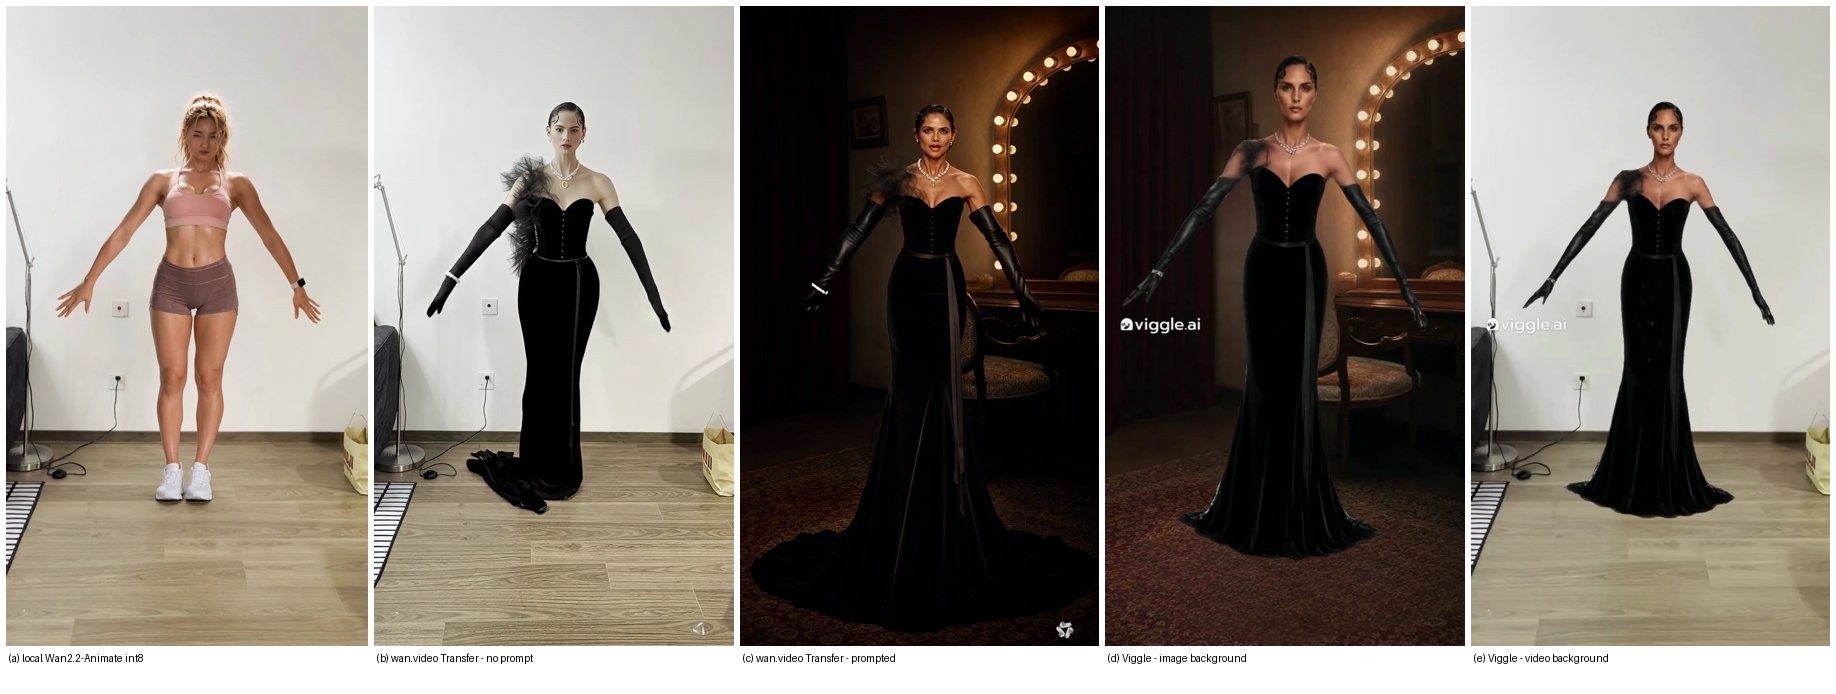
\includegraphics[width=\textwidth,height=0.85\textheight,keepaspectratio]{figs/hosted_service_comparison_contact_sheet.png}
\par\vspace{3pt}{\footnotesize \textbf{Figure 4.6} --- Hosted-service comparison, matched mid-action frames from the same driving performance (4--5 Aug 2026; human review only). (a) Local Wan2.2-Animate int8 run (Look 1 reference). (b) \texttt{wan.video} Transfer \emph{without} a prompt: the service silently kept the driving video's room and discarded the reference image's dressing-room scene. (c) The same service \emph{with} an explicit keep-the-image-background instruction: scene preserved. (d--e) Viggle free tier in image-background and video-background modes: identity drift, garment simplification and compositing artefacts are visible (service watermark present). The look references differ between (a) and (b--e), so quality differences are indicative, not controlled.}
\end{figure*}

\par\vspace{22pt}
\Needspace*{12\baselineskip}
\addcontentsline{toc}{section}{Chapter 5 --- Professional and Ethical Considerations}

\vspace*{2pt}\noindent{\LARGE\bfseries Chapter 5 --- Professional and Ethical Considerations\par}\vspace{3pt}\hrule height 0.8pt\vspace{12pt}

This chapter sets out the professional and ethical considerations that shaped the system's design and evaluation. Several are not incidental to the project but central to it: a system that regenerates video with a fixed character, and --- in Mode C --- replaces a filmed performer with a target character, sits close to well-known copyright and synthetic-media concerns, and the design choices in Chapters 3--4 were made partly to keep the work on the right side of those lines.

\addcontentsline{toc}{subsection}{5.1 Copyright and the extract-structure principle}

\section*{5.1 Copyright and the extract-structure principle}

The system is built on a single copyright-aware principle: \textbf{extract structure, regenerate content} (\S{}3.8). Reference clips are analysed only for \emph{formal structure} --- shot boundaries, cut rhythm, framing, a broad camera-motion class, body orientation and beat timing --- and none of the reference's pixels appear in the output. Reference audio is used solely to derive a beat grid and is never reproduced. The generated output uses an original, project-owned IP character, new scene prompts and royalty-free or self-created assets. Reference material is authorised, self-created or royalty-free.

This distinction matters because structure and expression are treated differently under copyright: a shot rhythm or a generic "walk toward the sunset" is closer to an unprotectable idea, whereas the literal footage is protected expression. The pipeline is deliberately confined to the former. This is stated in the dissertation as \textbf{risk reduction, not a legal guarantee} (\S{}4.15.1): a highly distinctive sequence of shots could still carry protectable selection-and-arrangement, character reference images must be owned or licensed, and the training data of the closed third-party models is not transparent. Where doubt exists, the safe reading is that the system reuses \emph{generic} structure, not a specific creative arrangement.

\addcontentsline{toc}{subsection}{5.2 Synthetic media, likeness and person replacement}

\section*{5.2 Synthetic media, likeness and person replacement}

Person-replacement generation is adjacent to the misuse space commonly labelled "deepfakes". The project addresses this directly rather than by omission.

First, the target character is a \textbf{fictional, project-owned IP identity}, not a real, named person. The system is not designed to impersonate a real individual, and the identity references are original assets. Second, in Mode C the \emph{driving} performance video does contain a real person (a consenting volunteer performing simple movements); that person's face is \textbf{pixelated/anonymised in every figure} in this dissertation (e.g. Figures 3.9 and 4.4), and the driving video supplies motion and body silhouette only --- not the performer's identity, which is replaced. Third, the honest finding that the system's identity control is \emph{imperfect} on a closed API (identity is "similar, not exact", \S{}4.12, \S{}4.17) is, in this context, a safety-relevant property rather than only a limitation: the system does not produce a convincing likeness of any specific real person.

The responsible-use position is therefore explicit: the appropriate applications are creator-owned character content and previsualisation, not the non-consensual replacement or impersonation of real people. A production version should add provenance signalling (for example, content credentials or visible synthetic-media labelling) and a consent record for any driving performer. These are noted as requirements for any deployment beyond this proof of concept.

\addcontentsline{toc}{subsection}{5.3 Data and consent}

\section*{5.3 Data and consent}

No third-party dataset is collected. The only real-person material is the Mode~C driving-performance video, recorded with the performer's consent and anonymised in dissertation figures; it is used only as motion-conditioning material. The remaining materials are original IP character references, the author-created AI-generated beach reference clip (used only as a structural source), and a static scene-asset package. No human-subject study was run --- the evaluation's "human review" is author-conducted inspection (\S{}4.15.2), which is disclosed as such rather than presented as an independent user study.

\addcontentsline{toc}{subsection}{5.4 Honesty, reproducibility and professional practice}

\section*{5.4 Honesty, reproducibility and professional practice}

A professional-practice commitment runs through the evaluation: an \textbf{executed-versus-pending} reporting rule under which no metric is invented, every number is traceable to an execution log, \texttt{ffprobe}, an optical-flow or ArcFace computation, or the decision log, and results the system did not produce are labelled pending rather than filled in. Negative results (the archived skeleton-guidance branch, \S{}4.12; the residual motion gap, \S{}4.13) are reported as findings, not hidden. This discipline is itself an ethical stance: it prevents the over-claiming that is common around generative-AI demonstrations and keeps the contribution defensible.

Two further professional considerations follow. The pipeline keeps a \textbf{human in the loop} at acceptance (\S{}4.15.1): generation is gated on human review rather than delegated wholly to an automatic metric that the identity audit (\S{}4.8.1) shows can misjudge a synthetic character. And the system is built for \textbf{auditability} --- every per-shot decision is written to a readable state file with an explicit \texttt{needs\_human} terminal state --- so that its behaviour can be inspected and reproduced rather than trusted blindly.

\addcontentsline{toc}{subsection}{5.5 Environmental and cost considerations}

\section*{5.5 Environmental and cost considerations}

The system performs no model training; it composes closed inference APIs and local CPU analysis. Its compute footprint is therefore modest and dominated by a small number of image- and video-generation API calls per shot, plus zero-cost local analysis (segmentation, pose, optical flow, ArcFace). The agentic repair loop increases the number of generation calls, which is both a cost and an environmental consideration; the dissertation reports attempt counts (eight generations for four approved shots, \S{}4.4) precisely so that this cost is visible rather than hidden, and identifies an equal-budget baseline as necessary future work (\S{}4.15.2).

\par\vspace{22pt}
\Needspace*{12\baselineskip}
\addcontentsline{toc}{section}{Chapter 6 --- Conclusion and Future Work}

\vspace*{2pt}\noindent{\LARGE\bfseries Chapter 6 --- Conclusion and Future Work\par}\vspace{3pt}\hrule height 0.8pt\vspace{12pt}

\addcontentsline{toc}{subsection}{6.1 Summary}

\section*{6.1 Summary}

This dissertation set out to determine whether a reference short-form video can be decomposed into a reusable structural template and regenerated with a fixed IP character, under both scene preservation and scene replacement, using an agentic evaluation--repair loop built only on closed generation APIs. A four-stage pipeline was designed and built to do this: deterministic reference analysis, a five-track beat-aligned storyboard, IP-conditioned keyframe-first per-shot regeneration with identity, look and scene separated, and an agentic evaluation--repair loop that repairs only the failed shot and logs every decision. The pipeline was demonstrated end to end on a four-shot beach reference under human review, with a decision log providing real evidence of self-correcting generation, and was exercised again under scene replacement into a Parisian street scene.

\addcontentsline{toc}{subsection}{6.2 What the evaluation showed}

\section*{6.2 What the evaluation showed}

Reported under an executed-versus-pending rule, the executed results include a complete end-to-end run (four keyframes generated and human-approved across eight logged attempts, assembled into a 768$\times$1152, 20.4 s vertical short); a log-reconstructed loop-off-versus-loop-on comparison in which first-attempt acceptance rose from 25\% to 100\% under gated repair; a motion-energy audit quantifying that single-keyframe animation reproduces 14--64\% of the reference's per-frame motion, improved on the two weakest shots by a prompt-only repair; and an identity-metric audit. The identity audit is the most instructive result: ArcFace cosine similarity under-scored keyframes that human review accepted as the same synthetic character, empirically confirming that a single embedding metric is mis-calibrated for a stylised IP identity and justifying the decision to gate acceptance on human review rather than one metric. A Phase 0 driving-video backend (Mode C) was shown to run on available hardware and to follow driving motion while preserving the background, confirming the reference-role boundary argued throughout (driving supplies motion and body; reference supplies appearance). Across every executed result in this chapter, the same boundary holds: the system preserves reference shot structure and action intent, but does not perform exact frame-level motion transfer.

\addcontentsline{toc}{subsection}{6.3 Reflection: negative results as findings}

\section*{6.3 Reflection: negative results as findings}

Two negative results are reported as engineering contributions rather than hidden. First, a pose skeleton supplied only as an image reference is too weak a control signal for the closed image-edit API, so the start/end-keyframe pose branch was tested and archived; reliable pose control requires a pose-conditioned backend. Second, single-keyframe image-to-video under-conditions the temporal sequence, since only the start frame is controlled. Both are direct evidence for \emph{why} an explicit orchestration and repair layer is needed rather than a direct API call, and, unlike a hosted interface, the pipeline's behaviour is recorded, evaluable and reproducible. A third, late-run piece of evidence points the same way from outside the pipeline: in the dated hosted-service comparison (\S{}4.18), an unprompted one-click service silently chose scene semantics on the user's behalf, and only an explicit instruction restored control --- the implicit-orchestration behaviour this dissertation argues an explicit pipeline must replace.

\addcontentsline{toc}{subsection}{6.4 Limitations}

\section*{6.4 Limitations}

The limitations are stated in full in \S{}4.15 and are not repeated here beyond their headline: the loop that operated was human-gated rather than fully automatic; the evaluation rests on one reference video and one character; there is no equal-budget baseline; automated framing and beat-alignment scores remain uncomputed; control-signal reliability varies by shot type (full-body shots yield usable pose/mask candidates where close-up and detail shots do not, \S{}4.11.1), and stronger temporal segmentation, tracking and control conditioning remain future work; and pixel-level output is bound to specific closed-model versions. These bound the claim to a proof of concept.

\addcontentsline{toc}{subsection}{6.5 Future work}

\section*{6.5 Future work}

Several extensions follow directly from the limitations. (1) \emph{Complete the automated metrics}: framing-accuracy and beat-alignment scores are computable at zero cost from the already-logged cut and beat timestamps, closing the last pending cells. (2) \emph{Close the automatic loop}: replace the human gate with automatic scoring$\rightarrow$diagnosis$\rightarrow$targeted repair, and run the controlled loop-off-versus-loop-on ablation with a matched attempt budget and a blind reviewer (\S{}4.12). (3) \emph{Stronger identity}: adopt IP-Adapter FaceID, InstantID or a trained LoRA to reduce identity drift beyond what reference-image ordering achieves on a closed API. (4) \emph{Stronger structural control}: move per-shot generation onto a pose-conditioned backend (ControlNet-style or a driving-video model), which the negative results identify as the route to reliable motion. (5) \emph{Mode C to completion}: full-length driving-video generation and the scene-regenerating Condition B. (6) \emph{Generalisation and a user study}: multiple characters, scenes and reference clips, evaluated with independent raters against matched baselines.

\addcontentsline{toc}{subsection}{6.6 Closing}

\section*{6.6 Closing}

The system is best understood as a proof of concept for auditable, reference-structured and selectively-repairable short-form video generation, not a system for exact motion transfer or autonomous cinematic production. Its contribution is an orchestration layer --- deterministic reference decomposition, identity/look/scene-separated per-shot regeneration, and an auditable agentic repair loop with a decision log --- reported with an honest account, negative results included, of where it works and where it does not.

\par\vspace{22pt}
\Needspace*{12\baselineskip}
\addcontentsline{toc}{section}{References}

\vspace*{2pt}\noindent{\LARGE\bfseries References\par}\vspace{3pt}\hrule height 0.8pt\vspace{12pt}

Blattmann, A., Dockhorn, T., Kulal, S., Mendelevitch, D., Kilian, M., Lorenz, D., Levi, Y., English, Z., Voleti, V., Letts, A., et al. (2023). Stable Video Diffusion: Scaling Latent Video Diffusion Models to Large Datasets. \emph{arXiv preprint arXiv:2311.15127}.

Bradski, G. (2000). The OpenCV Library. \emph{Dr.\ Dobb's Journal of Software Tools}. https://opencv.org

Castellano, B. (n.d.). \emph{PySceneDetect: Video Scene Cut Detection and Analysis Tool}. Software. Repository: https://github.com/Breakthrough/PySceneDetect. https://www.scenedetect.com

Cheng, G., Gao, X., et al. (2025). \emph{Wan-Animate: Unified Character Animation and Replacement with Holistic Replication}. Technical report, arXiv:2509.14055 (Wan Team, Alibaba Group). Release: https://github.com/Wan-Video/Wan2.2. https://arxiv.org/abs/2509.14055

DeepBeepMeep (2026). \emph{WanGP / Wan2GP: Low-VRAM Video Generation Runner} [Software]. Third-party low-VRAM runner used for the Wan2.2-Animate experiments; accessed 2026-08-05. https://github.com/deepbeepmeep/Wan2GP

Deng, J., Guo, J., Xue, N., \& Zafeiriou, S. (2019). ArcFace: Additive Angular Margin Loss for Deep Face Recognition. In \emph{Proceedings of the IEEE/CVF Conference on Computer Vision and Pattern Recognition (CVPR)}.

Farneb\"ack, G. (2003). Two-Frame Motion Estimation Based on Polynomial Expansion. In \emph{Scandinavian Conference on Image Analysis (SCIA)}.

FFmpeg developers (n.d.). \emph{FFmpeg: A Complete, Cross-Platform Solution to Record, Convert and Stream Audio and Video}. Software. https://ffmpeg.org

Gal, R., Alaluf, Y., Atzmon, Y., Patashnik, O., Bermano, A. H., Chechik, G., \& Cohen-Or, D. (2023). An Image is Worth One Word: Personalizing Text-to-Image Generation using Textual Inversion. In \emph{International Conference on Learning Representations (ICLR)}.

Guo, Y., Yang, C., Rao, A., Liang, Z., Wang, Y., Qiao, Y., Agrawala, M., Lin, D., \& Dai, B. (2024). AnimateDiff: Animate Your Personalized Text-to-Image Diffusion Models without Specific Tuning. In \emph{International Conference on Learning Representations (ICLR)}.

Hu, E. J., Shen, Y., Wallis, P., Allen-Zhu, Z., Li, Y., Wang, S., Wang, L., \& Chen, W. (2022). LoRA: Low-Rank Adaptation of Large Language Models. In \emph{International Conference on Learning Representations (ICLR)}.

Hu, L., Gao, X., Zhang, P., Sun, K., Zhang, B., \& Bo, L. (2023). Animate Anyone: Consistent and Controllable Image-to-Video Synthesis for Character Animation. \emph{arXiv preprint arXiv:2311.17117}.

InsightFace contributors (2026). \emph{InsightFace: 2D and 3D Face Analysis Project} [Software]. Implementation used for the ArcFace-style face-embedding diagnostics (\texttt{buffalo\_l} pack); accessed 2026-08-05. https://github.com/deepinsight/insightface

Kirillov, A., Mintun, E., Ravi, N., Mao, H., Rolland, C., Gustafson, L., Xiao, T., Whitehead, S., Berg, A. C., Lo, W.-Y., Doll\'ar, P., \& Girshick, R. (2023). Segment Anything. In \emph{Proceedings of the IEEE/CVF International Conference on Computer Vision (ICCV)}.

Kuaishou Technology (2024). \emph{Kling: Video Generation Model}. Vendor product, accessed 2026-07-23. https://klingai.com

Lasseter, J. (1987). Principles of Traditional Animation Applied to 3D Computer Animation. \emph{ACM SIGGRAPH Computer Graphics}, 21(4), 35--44.

Li, Z., Cao, M., Wang, X., Qi, Z., Cheng, M., \& Shan, Y. (2024). PhotoMaker: Customizing Realistic Human Photos via Stacked ID Embedding. In \emph{Proceedings of the IEEE/CVF Conference on Computer Vision and Pattern Recognition (CVPR)}.

Lugaresi, C., Tang, J., Nash, H., McClanahan, C., Uboweja, E., Hays, M., Zhang, F., Chang, C., Yong, M. G., Lee, J., et al. (2019). MediaPipe: A Framework for Building Perception Pipelines. \emph{arXiv preprint arXiv:1906.08172}.

Madaan, A., Tandon, N., Gupta, P., Hallinan, S., Gao, L., Wiegreffe, S., Alon, U., Dziri, N., Prabhumoye, S., Yang, Y., et al. (2023). Self-Refine: Iterative Refinement with Self-Feedback. In \emph{Advances in Neural Information Processing Systems (NeurIPS)}.

McFee, B., Raffel, C., Liang, D., Ellis, D. P. W., McVicar, M., Battenberg, E., \& Nieto, O. (2015). librosa: Audio and Music Signal Analysis in Python. In \emph{Proceedings of the 14th Python in Science Conference (SciPy)}.

Mou, C., Wang, X., Xie, L., Wu, Y., Zhang, J., Qi, Z., \& Shan, Y. (2024). T2I-Adapter: Learning Adapters to Dig out More Controllable Ability for Text-to-Image Diffusion Models. In \emph{Proceedings of the AAAI Conference on Artificial Intelligence (AAAI)}.

OpenAI (2024). \emph{Hello GPT-4o}. Vendor documentation, accessed 2026-08-05. https://openai.com/index/hello-gpt-4o/

OpenAI (2025). \emph{Introducing our latest image generation model in the API (gpt-image-1)}. Vendor documentation, accessed 2026-07-23. https://openai.com/index/image-generation-api/

Rother, C., Kolmogorov, V., \& Blake, A. (2004). ``GrabCut'': Interactive Foreground Extraction Using Iterated Graph Cuts. \emph{ACM Transactions on Graphics}, 23(3), 309--314.

Ruiz, N., Li, Y., Jampani, V., Pritch, Y., Rubinstein, M., \& Aberman, K. (2023). DreamBooth: Fine Tuning Text-to-Image Diffusion Models for Subject-Driven Generation. In \emph{Proceedings of the IEEE/CVF Conference on Computer Vision and Pattern Recognition (CVPR)}.

Shinn, N., Cassano, F., Berman, E., Gopinath, A., Narasimhan, K., \& Yao, S. (2023). Reflexion: Language Agents with Verbal Reinforcement Learning. In \emph{Advances in Neural Information Processing Systems (NeurIPS)}.

Thomas, F., \& Johnston, O. (1981). \emph{Disney Animation: The Illusion of Life}. Abbeville Press.

Wang, Q., Bai, X., Wang, H., Qin, Z., Chen, A., Li, H., Tang, X., \& Hu, Y. (2024). InstantID: Zero-shot Identity-Preserving Generation in Seconds. \emph{arXiv preprint arXiv:2401.07519}.

Williams, R. (2001). \emph{The Animator's Survival Kit}. Faber and Faber.

Xu, Z., Zhang, J., Liew, J. H., Yan, H., Liu, J., Zhang, C., Feng, J., \& Shou, M. Z. (2024). MagicAnimate: Temporally Consistent Human Image Animation using Diffusion Model. In \emph{Proceedings of the IEEE/CVF Conference on Computer Vision and Pattern Recognition (CVPR)}.

Yang, Z., Zeng, A., Yuan, C., \& Li, Y. (2023). Effective Whole-body Pose Estimation with Two-stages Distillation. In \emph{Proceedings of the IEEE/CVF International Conference on Computer Vision Workshops (ICCVW), CV4Metaverse}.

Yao, S., Zhao, J., Yu, D., Du, N., Shafran, I., Narasimhan, K., \& Cao, Y. (2023). ReAct: Synergizing Reasoning and Acting in Language Models. In \emph{International Conference on Learning Representations (ICLR)}.

Ye, H., Zhang, J., Liu, S., Han, X., \& Yang, W. (2023). IP-Adapter: Text Compatible Image Prompt Adapter for Text-to-Image Diffusion Models. \emph{arXiv preprint arXiv:2308.06721}.

Zhang, L., Rao, A., \& Agrawala, M. (2023). Adding Conditional Control to Text-to-Image Diffusion Models. In \emph{Proceedings of the IEEE/CVF International Conference on Computer Vision (ICCV)}.

\par\vspace{22pt}
\Needspace*{12\baselineskip}
\addcontentsline{toc}{section}{Appendix A --- Results Showcase}

\vspace*{2pt}\noindent{\LARGE\bfseries Appendix A --- Results Showcase\par}\vspace{3pt}\hrule height 0.8pt\vspace{12pt}

This appendix collects the concrete artefacts produced by the system so that the delivered work can be inspected directly rather than only described. All material is from the completed end-to-end beach run (\texttt{live\_test\_03\_4shots}), the strongest executed evidence in the dissertation; the figures are the system's own outputs, not illustrations.

\addcontentsline{toc}{subsection}{A.1 End-to-end output: the assembled beach short}

\section*{A.1 End-to-end output: the assembled beach short}

Figure A.1 samples the final assembled vertical short (768$\times$1152, 20.4 s) at even intervals across its four shots. The character identity, look (the charcoal-blazer "Look 3") and seaside scene hold across an over-shoulder close-up, a back-view walk, a low-angle feet insert and a side-profile walk --- the four shot types decomposed from the reference --- demonstrating the identity/look/scene consistency the pipeline is designed to preserve.

\begin{figure*}[!tp]
\centering
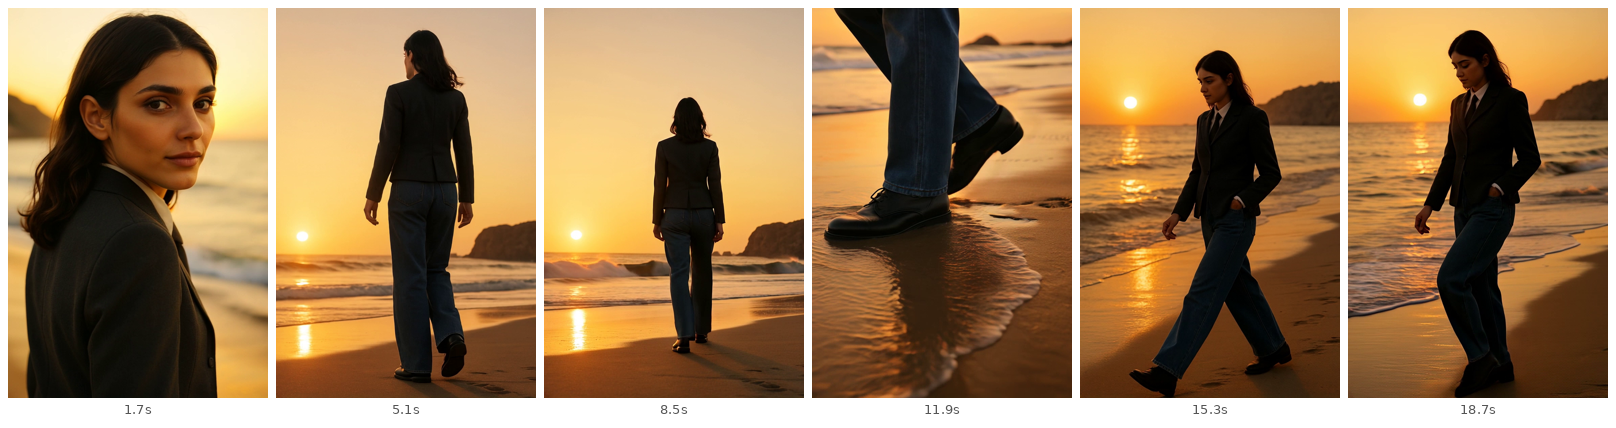
\includegraphics[width=\textwidth,height=0.85\textheight,keepaspectratio]{figs/beach_final_frame_grid.png}
\par\vspace{3pt}{\footnotesize \textbf{Figure A.1} --- Frame grid from the final assembled beach short (\texttt{final\_look3\_reference\_driven\_demo.mp4}), sampled at 1.7 s, 5.1 s, 8.5 s, 11.9 s, 15.3 s and 18.7 s. One coherent character across the four reference-derived shot types.}
\end{figure*}

\addcontentsline{toc}{subsection}{A.2 Approved keyframes}

\section*{A.2 Approved keyframes}

Figure A.2 is the keyframe contact sheet: the four per-shot keyframes that passed the human review gate and were then animated to video. These are the "key poses" of the pose-to-pose strategy (\S{}2.1), generated first and approved before any image-to-video step.

\begin{figure*}[!tp]
\centering
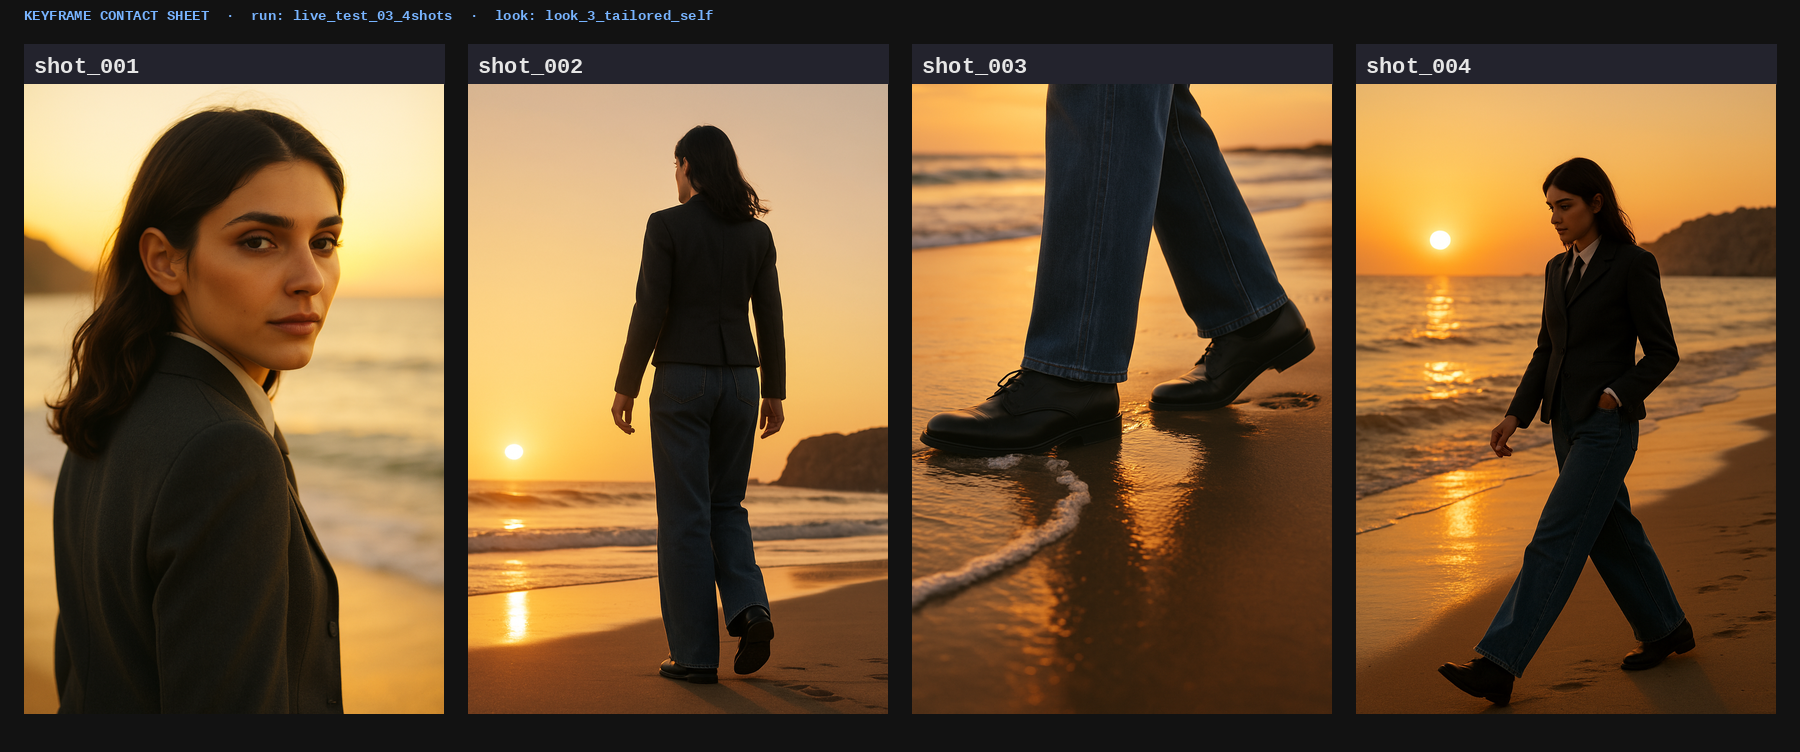
\includegraphics[width=\textwidth,height=0.85\textheight,keepaspectratio]{figs/beach_keyframe_contact_sheet.png}
\par\vspace{3pt}{\footnotesize \textbf{Figure A.2} --- The four approved keyframes (\texttt{gpt-image-1}, \texttt{images.edit}, 1024$\times$1536), one per shot, produced across eight logged generation attempts (1 / 2 / 2 / 3 per shot) before assembly.}
\end{figure*}

\addcontentsline{toc}{subsection}{A.3 Reference structure vs. regenerated content}

\section*{A.3 Reference structure vs. regenerated content}

Figure A.3 places the reference frames beside the regenerated keyframes for the same shots. It makes the central "extract structure, regenerate content" principle (\S{}3.8, \S{}5.1) visible: shot framing, body orientation and composition are carried over, while the character, look and rendered pixels are newly generated and share none of the reference's content.

\begin{figure*}[!tp]
\centering
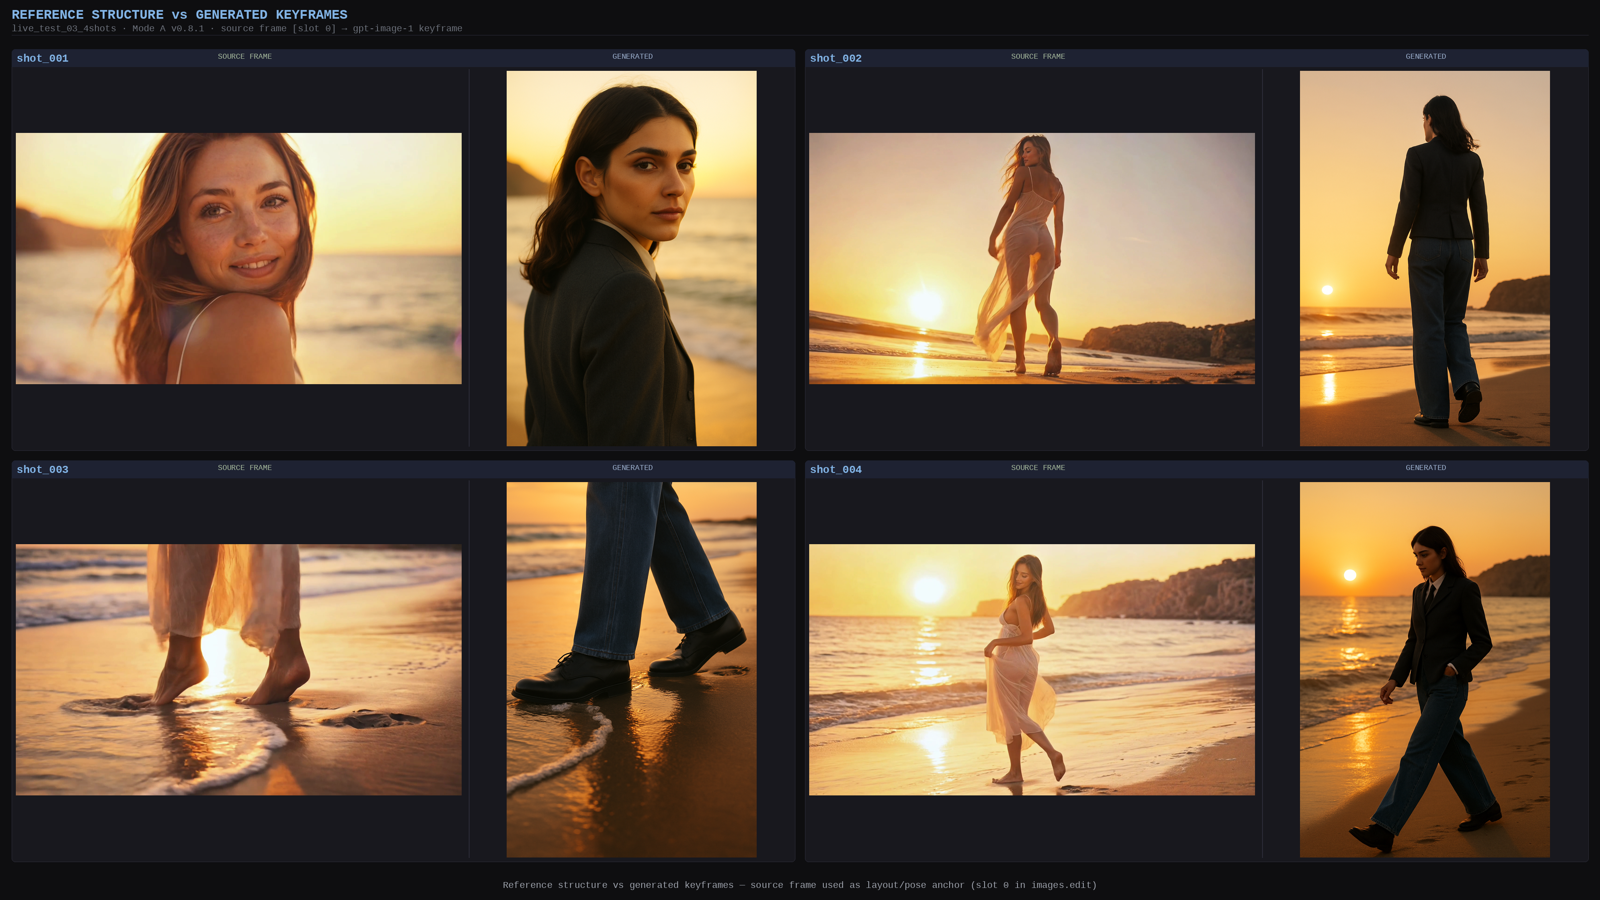
\includegraphics[width=\textwidth,height=0.85\textheight,keepaspectratio]{figs/reference_vs_keyframe.png}
\par\vspace{3pt}{\footnotesize \textbf{Figure A.3} --- Reference frames (top) vs. the system's regenerated keyframes (bottom) for the corresponding shots. Structure is reused; content is regenerated with the project-owned IP character.}
\end{figure*}

\addcontentsline{toc}{subsection}{A.4 Decision-log excerpt (state file)}

\section*{A.4 Decision-log excerpt (state file)}

The pipeline's agentic behaviour is recorded in a single readable state file, \texttt{decision\_log.json}. The excerpt below is the record for \texttt{shot\_002} exactly as written by the run --- the shot whose first keyframe attempt was blocked by the pre-API forbidden-word guard and regenerated. It shows the fields that make the loop auditable: the generation attempt count and diagnosis, the I2V record, and --- under the executed-versus-pending reporting rule --- the automatic-evaluation state left honestly as \texttt{pending} rather than fabricated.

\begin{quotebox}\texttt{shot\_id}: shot\_002 $\cdot$ \texttt{framing}: wide \texttt{keyframe\_generation}: \{ \texttt{attempts}: 2, \texttt{status}: approved, \texttt{model}: gpt-image-1 / images.edit / 1024$\times$1536, \texttt{notes}: "v1 blocked by forbidden-word guard (bride/bridal in negative instructions); v2 natural-realism language, approved" \} \texttt{kling\_i2v}: \{ \texttt{model}: kling-v1-6 / std / 9:16 / 5s, \texttt{motion\_type}: prompt-level I2V (not pose transfer), \texttt{status}: success \} \texttt{evaluation}: \{ \texttt{status}: pending, \texttt{note}: "Evaluation not yet run. Awaiting user approval to start." \} \texttt{repair}: \{ \texttt{status}: not\_run, \texttt{note}: "No repair triggered --- evaluation pending." \}\end{quotebox}

Across the four shots the state file records eight keyframe-generation attempts (1 / 2 / 2 / 3), each diagnosed and repaired at the keyframe stage under human review, four successful I2V clips, and a consistent \texttt{evaluation: pending} state --- the complete, honest decision record that doubles as the dissertation's evaluation data (\S{}4.4, \S{}4.9).

\end{document}
